% generated by GAPDoc2LaTeX from XML source (Frank Luebeck)
\documentclass[a4paper,11pt]{report}

\usepackage[top=37mm,bottom=37mm,left=27mm,right=27mm]{geometry}
\sloppy
\pagestyle{myheadings}
\usepackage{amssymb}
\usepackage[utf8]{inputenc}
\usepackage{makeidx}
\makeindex
\usepackage{color}
\definecolor{FireBrick}{rgb}{0.5812,0.0074,0.0083}
\definecolor{RoyalBlue}{rgb}{0.0236,0.0894,0.6179}
\definecolor{RoyalGreen}{rgb}{0.0236,0.6179,0.0894}
\definecolor{RoyalRed}{rgb}{0.6179,0.0236,0.0894}
\definecolor{LightBlue}{rgb}{0.8544,0.9511,1.0000}
\definecolor{Black}{rgb}{0.0,0.0,0.0}

\definecolor{linkColor}{rgb}{0.0,0.0,0.554}
\definecolor{citeColor}{rgb}{0.0,0.0,0.554}
\definecolor{fileColor}{rgb}{0.0,0.0,0.554}
\definecolor{urlColor}{rgb}{0.0,0.0,0.554}
\definecolor{promptColor}{rgb}{0.0,0.0,0.589}
\definecolor{brkpromptColor}{rgb}{0.589,0.0,0.0}
\definecolor{gapinputColor}{rgb}{0.589,0.0,0.0}
\definecolor{gapoutputColor}{rgb}{0.0,0.0,0.0}

%%  for a long time these were red and blue by default,
%%  now black, but keep variables to overwrite
\definecolor{FuncColor}{rgb}{0.0,0.0,0.0}
%% strange name because of pdflatex bug:
\definecolor{Chapter }{rgb}{0.0,0.0,0.0}
\definecolor{DarkOlive}{rgb}{0.1047,0.2412,0.0064}


\usepackage{fancyvrb}

\usepackage{mathptmx,helvet}
\usepackage[T1]{fontenc}
\usepackage{textcomp}


\usepackage[
            pdftex=true,
            bookmarks=true,        
            a4paper=true,
            pdftitle={Written with GAPDoc},
            pdfcreator={LaTeX with hyperref package / GAPDoc},
            colorlinks=true,
            backref=page,
            breaklinks=true,
            linkcolor=linkColor,
            citecolor=citeColor,
            filecolor=fileColor,
            urlcolor=urlColor,
            pdfpagemode={UseNone}, 
           ]{hyperref}

\newcommand{\maintitlesize}{\fontsize{50}{55}\selectfont}

% write page numbers to a .pnr log file for online help
\newwrite\pagenrlog
\immediate\openout\pagenrlog =\jobname.pnr
\immediate\write\pagenrlog{PAGENRS := [}
\newcommand{\logpage}[1]{\protect\write\pagenrlog{#1, \thepage,}}
%% were never documented, give conflicts with some additional packages

\newcommand{\GAP}{\textsf{GAP}}

%% nicer description environments, allows long labels
\usepackage{enumitem}
\setdescription{style=nextline}

%% depth of toc
\setcounter{tocdepth}{1}

% This document contains the TikZ-header for all our LaTeX-computations.
% It especially contains all global graphic parameters.

\usepackage{amsmath, amssymb, amsfonts} % Standard Math-stuff

\usepackage{ifthen}

\usepackage{tikz}
\usetikzlibrary{calc}
\usetikzlibrary{positioning}
\usetikzlibrary{shapes}
\usetikzlibrary{patterns}


% Sometimes we want to implement different behaviour for the generated 
% HTML-pictures (for example, shading is not supported in HTML).
% For that we define a macro to check whether we run the code with
% htlatex. The code comes from 
% https://tex.stackexchange.com/questions/93852/what-is-the-correct-way-to-check-for-latex-pdflatex-and-html-in-the-same-latex
\makeatletter
\edef\texforht{TT\noexpand\fi
  \@ifpackageloaded{tex4ht}
    {\noexpand\iftrue}
    {\noexpand\iffalse}}
\makeatother


% Define a text=none option for nodes that ignores the given text, from
% https://tex.stackexchange.com/questions/59354/no-text-none-in-tikz
\makeatletter
\newif\iftikz@node@phantom
\tikzset{
  phantom/.is if=tikz@node@phantom,
  text/.code=%
    \edef\tikz@temp{#1}%
    \ifx\tikz@temp\tikz@nonetext
      \tikz@node@phantomtrue
    \else
      \tikz@node@phantomfalse
      \let\tikz@textcolor\tikz@temp
    \fi
}
\usepackage{etoolbox}
\patchcmd\tikz@fig@continue{\tikz@node@transformations}{%
  \iftikz@node@phantom
    \setbox\pgfnodeparttextbox\hbox{}
  \fi\tikz@node@transformations}{}{}
\makeatother

% Find the angle of a given line (within TikZ)
\newcommand{\tikzAngleOfLine}{\tikz@AngleOfLine}
\def\tikz@AngleOfLine(#1)(#2)#3{%
  \pgfmathanglebetweenpoints{%
    \pgfpointanchor{#1}{center}}{%
    \pgfpointanchor{#2}{center}}
  \pgfmathsetmacro{#3}{\pgfmathresult}%
}

% Now we define the global styles
% The global styles are defined nestedly. You have to give your tikzpicture
% the global options [vertexStyle, edgeStyle, faceStyle] to activate them.
% 
% You can disable labels by using the option nolabels, i.e. 
% vertexStyle=nolabels to deactivate vertex labels.
%
% If you want to have a specific style for your picture, you can also use
% this specific meta-style instead of the general style. For example if you
% want to use double edges in one single picture - no matter the style of
% the rest of the document - you can use edgeDouble instead of edgeStyle.
%
% To set the default style, modify the vertexStyle/.default entry.

% Vertex styles
\tikzset{ 
    vertexNodePlain/.style = {fill=#1, shape=circle, inner sep=0pt, minimum size=2pt, text=none},
    vertexNodePlain/.default=gray,
    vertexPlain/labels/.style = {
        vertexNode/.style={vertexNodePlain=##1},
        vertexLabel/.style={gray}
    },
    vertexPlain/nolabels/.style = {
        vertexNode/.style={vertexNodePlain=##1},
        vertexLabel/.style={text=none}
    },
    vertexPlain/.style = vertexPlain/#1,
    vertexPlain/.default=labels
}
\tikzset{
    vertexNodeNormal/.style = {fill=#1, shape=circle, inner sep=0pt, minimum size=4pt, text=none},
    vertexNodeNormal/.default = blue,
    vertexNormal/labels/.style = {
        vertexNode/.style={vertexNodeNormal=##1},
        vertexLabel/.style={blue}
    },
    vertexNormal/nolabels/.style = {
        vertexNode/.style={vertexNodeNormal=##1},
        vertexLabel/.style={text=none}
    },
    vertexNormal/.style = vertexNormal/#1,
    vertexNormal/.default=labels
}
\tikzset{
    vertexNodeBallShading/pdf/.style = {ball color=#1},
    vertexNodeBallShading/svg/.style = {fill=#1},
    vertexNodeBallShading/.code = {% Conditional shading depending whether we want pdf or svg output
        \if\texforht
            \tikzset{vertexNodeBallShading/svg=#1!90!black}
        \else
            \tikzset{vertexNodeBallShading/pdf=#1}
        \fi
    },
    vertexNodeBall/.style = {shape=circle, vertexNodeBallShading=#1, inner sep=2pt, outer sep=0pt, minimum size=3pt, font=\tiny},
    vertexNodeBall/.default = white,
    vertexBall/labels/.style = {
        vertexNode/.style={vertexNodeBall=##1, text=black},
        vertexLabel/.style={text=none}
    },
    vertexBall/nolabels/.style = {
        vertexNode/.style={vertexNodeBall=##1, text=none},
        vertexLabel/.style={text=none}
    },
    vertexBall/.style = vertexBall/#1,
    vertexBall/.default=labels
}
\tikzset{ 
    vertexStyle/.style={vertexNormal=#1},
    vertexStyle/.default = labels
}


% 1) optional: colour of vertex
% 2) position of the vertex
% 3) relative position of the node
% 4) name of the vertex
\newcommand{\vertexLabelR}[4][]{
    \ifthenelse{ \equal{#1}{} }
        { \node[vertexNode] at (#2) {#4}; }
        { \node[vertexNode=#1] at (#2) {#4}; }
    \node[vertexLabel, #3] at (#2) {#4};
}
% 1) optional: colour of vertex
% 2) position of the vertex
% 3) absolute position of the node
% 4) name of the vertex
\newcommand{\vertexLabelA}[4][]{
    \ifthenelse{ \equal{#1}{} }
        { \node[vertexNode] at (#2) {#4}; }
        { \node[vertexNode=#1] at (#2) {#4}; }
    \node[vertexLabel] at (#3) {#4};
}


% Edge styles
% If you have trouble with the double-lines overlapping, this might (?) help:
% https://tex.stackexchange.com/questions/288159/closing-the-ends-of-double-line-in-tikz
\newcommand{\edgeLabelColor}{blue!20!white}
\tikzset{
    edgeLineNone/.style = {draw=none},
    edgeLineNone/.default=black,
    edgeNone/labels/.style = {
        edge/.style = {edgeLineNone=##1},
        edgeLabel/.style = {fill=\edgeLabelColor,font=\small}
    },
    edgeNone/nolabels/.style = {
        edge/.style = {edgeLineNone=##1},
        edgeLabel/.style = {text=none}
    },
    edgeNone/.style = edgeNone/#1,
    edgeNone/.default = labels
}
\tikzset{
    edgeLinePlain/.style={line join=round, draw=#1},
    edgeLinePlain/.default=black,
    edgePlain/labels/.style = {
        edge/.style={edgeLinePlain=##1},
        edgeLabel/.style={fill=\edgeLabelColor,font=\small}
    },
    edgePlain/nolabels/.style = {
        edge/.style={edgeLinePlain=##1},
        edgeLabel/.style={text=none}
    },
    edgePlain/.style = edgePlain/#1,
    edgePlain/.default = labels
}
\tikzset{
    edgeLineDouble/.style = {very thin, double=#1, double distance=.8pt, line join=round},
    edgeLineDouble/.default=gray!90!white,
    edgeDouble/labels/.style = {
        edge/.style = {edgeLineDouble=##1},
        edgeLabel/.style = {fill=\edgeLabelColor,font=\small}
    },
    edgeDouble/nolabels/.style = {
        edge/.style = {edgeLineDouble=##1},
        edgeLabel/.style = {text=none}
    },
    edgeDouble/.style = edgeDouble/#1,
    edgeDouble/.default = labels
}
\tikzset{
    edgeStyle/.style = {edgePlain=#1},
    edgeStyle/.default = labels
}

% Face styles
% Here we have an exception - the style face is always defined.
% 
\newcommand{\faceColorY}{yellow!60!white}   % yellow
\newcommand{\faceColorB}{blue!60!white}     % blue
\newcommand{\faceColorC}{cyan!60}           % cyan
\newcommand{\faceColorR}{red!60!white}      % red
\newcommand{\faceColorG}{green!60!white}    % green
\newcommand{\faceColorO}{orange!50!yellow!70!white} % orange

% define default face colour (and default swap colour)
\newcommand{\faceColor}{\faceColorY}
\newcommand{\faceColorSwap}{\faceColorC}

% define secondary default colours (to use in a single section)
\newcommand{\faceColorFirst}{green!40!white}
\newcommand{\faceColorSecond}{gray!15!white}
\newcommand{\faceColorThird}{red!17!white}
\newcommand{\faceColorFourth}{olive!20!white}

\tikzset{
    face/.style = {fill=#1},
    face/.default = \faceColor,
    faceY/.style = {face=\faceColorY},
    faceB/.style = {face=\faceColorB},
    faceC/.style = {face=\faceColorC},
    faceR/.style = {face=\faceColorR},
    faceG/.style = {face=\faceColorG},
    faceO/.style = {face=\faceColorO}
}
\tikzset{
    faceStyle/labels/.style = {
        faceLabel/.style = {}
    },
    faceStyle/nolabels/.style = {
        faceLabel/.style = {text=none}
    },
    faceStyle/.style = faceStyle/#1,
    faceStyle/.default = labels
}
\tikzset{ face/.style={fill=#1} }
\tikzset{ faceSwap/.code=
    \ifdefined\swapColors
        \tikzset{face=\faceColorSwap}
    \else
        \tikzset{face=\faceColor}
    \fi
}



\usepackage{hyperref}






%% command for ColorPrompt style examples
\newcommand{\gapprompt}[1]{\color{promptColor}{\bfseries #1}}
\newcommand{\gapbrkprompt}[1]{\color{brkpromptColor}{\bfseries #1}}
\newcommand{\gapinput}[1]{\color{gapinputColor}{#1}}


\begin{document}


\logpage{[ 0, 0, 0 ]}
\begin{titlepage}
\mbox{}\vfill

\begin{center}{\maintitlesize \textbf{ SimplicialSurfaces \mbox{}}}\\
\vfill

\hypersetup{pdftitle= SimplicialSurfaces }
\markright{\scriptsize \mbox{}\hfill  SimplicialSurfaces  \hfill\mbox{}}
{\Huge \textbf{ A tutorial for the SimplicialSurfaces-package. \mbox{}}}\\
\vfill

{\Huge  0.1 \mbox{}}\\[1cm]
{ 25 Oktober 2022 \mbox{}}\\[1cm]
\mbox{}\\[2cm]
{\Large \textbf{ Reymond Akpanya\\
    \mbox{}}}\\
{\Large \textbf{ Alice Niemeyer\\
    \mbox{}}}\\
{\Large \textbf{ Wilhelm Plesken\\
   \mbox{}}}\\

\hypersetup{pdfauthor= Reymond Akpanya\\
    ;  Alice Niemeyer\\
    ;  Wilhelm Plesken\\
   }
\end{center}\vfill

\mbox{}\\
{\mbox{}\\
\small \noindent \textbf{ Alice Niemeyer\\
    }  Email: \href{mailto://Alice.Niemeyer@Mathb.RWTH-Aachen.De} {\texttt{Alice.Niemeyer@Mathb.RWTH-Aachen.De}}\\
  Homepage: \href{http://www.math.rwth-aachen.de/~Alice.Niemeyer/} {\texttt{http://www.math.rwth-aachen.de/\texttt{\symbol{126}}Alice.Niemeyer/}}\\
  Address: \begin{minipage}[t]{8cm}\noindent
 Alice Niemeyer\\
 Lehrstuhl f{\"u}r Algebra und Darstellungstheorie\\
 RWTH Aachen\\
 Pontdriesch 10/16\\
 52062 Aachen\\
 GERMANY\\
 \end{minipage}
}\\
{\mbox{}\\
\small \noindent \textbf{ Reymond Akpanya\\
   }  Email: \href{mailto://akpanya@art.rwth-aachen.de} {\texttt{akpanya@art.rwth-aachen.de}}\\
  Address: \begin{minipage}[t]{8cm}\noindent
 --\\
 \end{minipage}
}\\
\end{titlepage}

\newpage\setcounter{page}{2}
{\small 
\section*{Copyright}
\logpage{[ 0, 0, 1 ]}
 {\copyright} 2016-2021 by Alice Niemeyer and Markus Baumeister

 The SimplicialSurfaces-package may be distributed under the terms and conditions of the GNU
Public License Version 3 (or higher).

The primary sources for much of the covered material are:

The PhD-thesis "Regularity Aspects for Combinatorial Simplicial Surfaces" of
Markus Baumeister

The book "Simplicial Surfaces of Congruent Triangles" by Alice C. Niemeyer,
Wilhelm Plesken, Daniel Robertz, and Ansgar W. Strzelczyk (unpublished)

 \mbox{}}\\[1cm]

\chapter{\textcolor{Chapter }{Tutorial}}\label{Chapter_Tutorial}
\logpage{[ 3, 0, 0 ]}
\hyperdef{L}{X81932F777898AD72}{}
{
  This chapter deals with the targeted use of the \texttt{SimplicialSurfaces} package to solve certain problems of interest. The aim of this tutorial is to
demonstrate the power of the package by combining several functions provided
in the package. It should enable users to find routines for their tasks
quickly without prior knowledge of the functions' names and also help users to
familiarise themselves with the package without having to read the entire
reference manual. 

 
\section{\textcolor{Chapter }{Parallelelepiped}}\label{Section_Parallelelepiped}
\logpage{[ 3, 1, 0 ]}
\hyperdef{L}{X855831967C42382F}{}
{
  

 $Problems:$ Construction of the simplicial parallelepiped 
\begin{enumerate}
\item  from a cube 
\item  from an octahedron and two tetrahedra via vertices in faces
\item  from an octahedron and two tetrahedra via surface constructions 
\item  from a double-6-gon using edge-turns 
\item  from a barycentric subdivision using edge-turns
\item  using the powerset of [1,2,3] as vertices
\end{enumerate}
 $Theoretical$ $background$ 
\begin{itemize}
\item  Vertex-faithful surfaces and boolean operations 
\end{itemize}
 

 $Frequently$ $used$ $commands$ 
\begin{itemize}
\item  ConnectedFaceSum() (\ref{ConnectedFaceSum}) 
\item  EdgesOfFaces() (local version: EdgesOfFace()) (\ref{EdgesOfFaces}) 
\item  EdgesOfVertices() (local version: Edges) (\ref{EdgesOfVertices}) 
\item  EulerCharacteristic() (\ref{EulerCharacteristic}) 
\item  FaceDegreesOfVertices() (local version: FaceDegreeOfVertex)(\ref{FaceDegreesOfVertices}) 
\item  FacesOfVertices() (local version: FacesOfVertex()) (\ref{FacesOfVertices}) 
\item  Flags() (\ref{Flags}) 
\item  IsIsomorphic() (\ref{IsIsomorphic}) 
\item  JoinBoundaries() (\ref{JoinBoundaries}) 
\item  NeighbourVerticesOfVertex() (\ref{NeighbourVerticesOfVertex}), 
\item  SimplicialSurfaceByVerticesInFaces() (works for vertex-faithful surfaces only)
(\ref{PolygonalStructures_surface}) 
\item  SubcomplexByFaces() (\ref{SubcomplexByFaces}) 
\item  VertexCounter() (local version: DegreeOfVertex()) (\ref{VertexCounter}) 
\item  VerticesOfEdges() (local Version: VerticesOfEdge()) (\ref{VerticesOfEdges}) 
\item  VerticesOfFaces() (local Version: VerticesOfFace()) (\ref{VerticesOfFaces}) 
\item  UmbrellaPathsOfVertices() (local version: UmbrellaPathOfVertex()) (\ref{UmbrellaPathsOfVertices}) 
\end{itemize}
 $Less$ $frequently$ $used$ $commands$ 
\begin{itemize}
\item  Cube() (\ref{Cube}) 
\item  JanusHead() (\ref{JanusHead}) 
\end{itemize}
 

 $ Mathematical$ $details:$ 

 A parallelepiped is a three dimensional convex body. In this exercise we shall
deal with its surface which we shall refer to as the ordinary parallelepiped,
and with a triangulation of it, which we shall call the simplicial
parallelepiped. Both are treated from a combinatorial point of view. 
\begin{center}
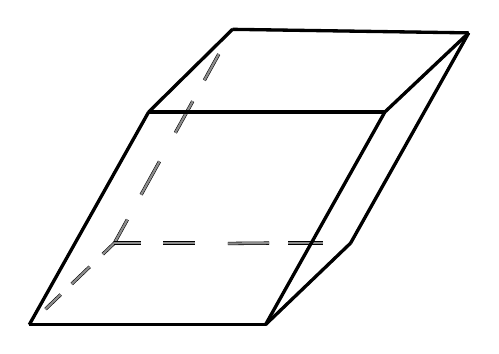
\begin{tikzpicture}[vertexBall, edgeDouble, faceStyle, scale=0.75]



\draw [edge] (-0.56,1.38)-- (-0.34006337147329324,1.7780852976333392);
\draw [edge] (-0.56,1.38)-- (-0.7558422406285278,1.192317852730994);
\draw [edge] (-0.56,1.38)-- (-0.1136851728156173,1.38);
\draw [edge] (0.26404404531757364,1.38)-- (0.8020220226587851,1.38);
\draw [edge] (1.3628926798868564,1.3737490708048605)-- (2.061119416436088,1.38);
\draw [edge] (2.3816169348521288,1.38)-- (2.9653802719670606,1.38);
\draw [edge] (-0.10675194529772192,2.2003789790111234)-- (0.20343768372046567,2.761822207534043);
\draw [edge] (0.4728326117873485,3.2494270273351007)-- (0.7674699302722631,3.7827205737927962);
\draw [edge] (0.9636806638503882,4.137862001569203)-- (1.2078332014992397,4.579778094713624);
\draw [edge] (-0.9791855203619909,0.9782805429864253)-- (-1.2823945953836728,0.6877051794239802);
\draw [edge] (-1.4693480282334692,0.5085414729429253)-- (-1.7266576066903034,0.2619531269217925);
\draw [edge=black] (2,0)-- (4.02,3.6);
\draw [edge=black] (0.02,3.6)-- (-2,0);
\draw [edge=black] (3.44,1.38)-- (5.44,4.94);
\draw [edge=black] (-2,0)-- (2,0);
\draw [edge=black] (2,0)-- (3.44,1.38);
\draw [edge=black] (1.44,5)-- (0.02,3.6);
\draw [edge=black] (0.02,3.6)-- (4.02,3.6);
\draw [edge=black] (4.02,3.6)-- (5.44,4.94);
\draw [edge=black] (5.44,4.94)-- (1.44,5);
\end{tikzpicture}

\end{center}
 We use a tetrahedron to triangulate the surface of a ordinary parallelepiped.
In this way each face is subdivided into 2 triangles and thus a simplicial
parallelepiped with 12 faces is constructed. So after triangulating, the
simplicial parallelepiped has more embeddings into three dimensional space,
since the original faces might be bent along the new edges. 
\begin{center}
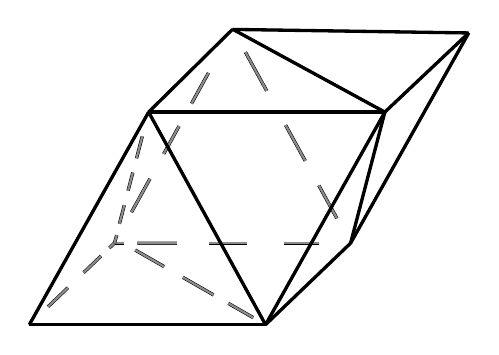
\begin{tikzpicture}[vertexBall, edgeDouble, faceStyle, scale=0.75]

\draw [edge=black] (-2,0)-- (2,0);

\draw [edge=black] (4.02,3.6)-- (0.02,3.6);
\draw [edge=black] (0.02,3.6)-- (-2,0);
\draw [edge=black] (3.44,1.38)-- (5.44,4.94);
\draw [edge=black] (5.44,4.94)-- (1.44,5);
\draw [edge=black] (2,0)-- (3.44,1.38);
\draw [edge=black] (1.44,5)-- (0.02,3.6);
\draw [edge=black] (4.02,3.6)-- (5.44,4.94);
\draw [edge] (1.0332274736325155,4.263741727274853)-- (0.7467514791515633,3.7452201772643297);
\draw [edge] (0.5353438881223546,3.362572437501462)-- (0.27515352774724633,2.891627885222516);
\draw [edge] (0.04213746170575994,2.4698688056874256)-- (-0.2706241668810365,1.903770257945324);
\draw [edge] (-0.17237103195467773,1.380053770842896)-- (0.5,1.38);
\draw [edge] (1.04,1.38)-- (1.68,1.38);
\draw [edge] (2.32,1.38)-- (2.9,1.38);
\draw [edge] (-0.7850135746606335,1.1643619909502263)-- (-1.0803981900452488,0.8812850678733032);
\draw [edge] (-1.3462443438914027,0.6265158371040724)-- (-1.68289592760181,0.303891402714932);
\draw [edge=black] (1.445708891887561,5.001217790538086)-- (4.02,3.6);
\draw [edge=black] (4.02,3.6)-- (3.44,1.38);
\draw [edge] (-0.20657687221433152,1.2634432090904641)-- (0.28208649654699514,0.9836440221384141);
\draw [edge] (0.6006954988489983,0.801214674046138)-- (1.1194827839545476,0.5041671156389285);
\draw [edge] (1.3693663636853701,0.3610886143414413)-- (1.7904098214480486,0.12000727965474631);
\draw [edge] (1.6586800662532202,4.614506441153063)-- (2.0193178570905728,3.9596632345578975);
\draw [edge] (2.3391022653831035,3.3790012721517955)-- (2.672007457959911,2.7745146949325603);
\draw [edge] (2.901332820391631,2.35810754209451)-- (3.209287291452826,1.7989262847814618);
\draw [edge] (-0.08740460161040448,3.1888996283187967)-- (-0.18448630955407658,2.817311022051638);
\draw [edge] (-0.24757816479935152,2.57582150714731)-- (-0.327664946393825,2.2692824465615664);
\draw [edge] (-0.47394672494161083,1.7093763286717656)-- (-0.39168935199695565,2.024223514770273);
\draw [edge] (-0.56,1.38)-- (-0.4,1.38);
\draw [edge] (-0.56,1.38)-- (-0.6456793566202854,1.2978906165722264);
\draw [edge] (-0.56,1.38)-- (-0.5195862057533234,1.5160463805806987);
\draw [edge=black] (2,0)-- (0.02,3.6);
\draw [edge=black] (2,0)-- (4.02,3.6);

\end{tikzpicture}



\end{center}
 Given a set of three linearly independent vectors in real 3-space, we can see
that they define a parallelepiped as well as a tetrahedron. 

 Note: Since we are only interested in surfaces, we shall refer to terms like
tetrahedron, parallelepiped, octahedron etc. as the boundary surfaces of these
three dimensional bodies, or rather to the combinatorial devices describing
their combinatorial structure. So instead of working with an embedding of
those structures, we see them as abstract surfaces represented by their
incidence geometry. 
\begin{center}


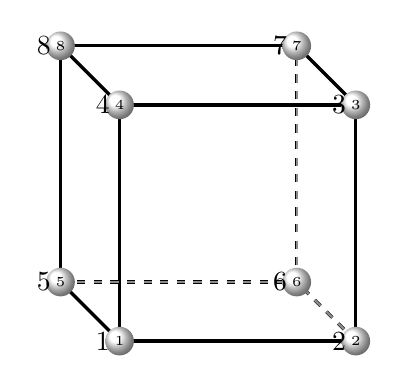
\begin{tikzpicture}[vertexBall, edgeDouble, faceStyle, scale=0.75]

% Define the coordinates of the vertices
\coordinate (V1_1) at (0, 0);
\coordinate (V2_1) at (4, 0);
\coordinate (V3_1) at (4,4);
\coordinate (V4_1) at (0,4);
\coordinate (V5_1) at (-1,1);
\coordinate (V6_1) at (3,1);
\coordinate (V7_1) at (3,5);
\coordinate (V8_1) at (-1,5);

\draw [edge=black] (0,0)-- (4,0);
\draw [edge=black] (4,0)-- (4,4);
\draw [edge=black] (4,4)-- (0,4);
\draw [edge=black] (0,4)-- (0,0);
\draw [edge=black] (-1,5)-- (-1,1);
\draw [dashed, edge] (-1,1)-- (3,1);
\draw [dashed, edge] (3,1)-- (3,5);
\draw [edge=black] (3,5)-- (-1,5);
\draw [edge=black] (0,0)-- (-1,1);
\draw [dashed, edge] (4,0)-- (3,1);
\draw [edge=black] (4,4)-- (3,5);
\draw [edge=black] (0,4)-- (-1,5);

\vertexLabelR{V1_1}{left}{$1$}
\vertexLabelR{V2_1}{left}{$2$}
\vertexLabelR{V3_1}{left}{$3$}
\vertexLabelR{V4_1}{left}{$4$}
\vertexLabelR{V5_1}{left}{$5$}
\vertexLabelR{V6_1}{left}{$6$}
\vertexLabelR{V7_1}{left}{$7$}
\vertexLabelR{V8_1}{left}{$8$}

\end{tikzpicture}



\end{center}
 Note: The \texttt{SimplicialSurfaces} package also contains functionalities to deal with polygonal complexes like
the cube and the ordinary parallelepiped. But since their combinatorial
structures do not differ, the simplicial parallelepiped is of greater interest
to us. 

 
\begin{Verbatim}[commandchars=!@|,fontsize=\small,frame=single,label=Example]
  !gapprompt@gap>| !gapinput@PE:=PolygonalComplexByVerticesInFaces([[1,2,3,4],[5,6,7,8],[1,2,5,6],|
  [2,3,6,7],[3,4,7,8],[1,4,5,8]]);
  polygonal surface (8 vertices, 12 edges, and 6 faces)  
  !gapprompt@gap>| !gapinput@IsIsomorphic(PE,Cube());|
  true
  !gapprompt@gap>| !gapinput@VerticesOfFaces(Cube());|
  [ [ 1, 2, 3, 4 ], [ 1, 2, 5, 6 ], [ 2, 3, 6, 7 ], [ 1, 4, 5, 8 ], 
   [ 3, 4, 7, 8 ], [ 5, 6, 7, 8 ] ]
  !gapprompt@gap>| !gapinput@VerticesOfFaces(PE);|
  [ [ 1, 2, 3, 4 ], [ 5, 6, 7, 8 ], [ 1, 2, 5, 6 ], [ 2, 3, 6, 7 ], 
   [ 3, 4, 7, 8 ], [ 1, 4, 5, 8 ] ]
\end{Verbatim}
 

 
\subsection{\textcolor{Chapter }{Construction from a cube}}\label{Chapter_Tutorial_Section_Parallelelepiped_Subsection_Construction_from_a_cube}
\logpage{[ 3, 1, 1 ]}
\hyperdef{L}{X7B23587684D03590}{}
{
  

 $Idea$ $behind$ $the$ $construcion$ 

 We construct a simplicial parallelepiped out of the combinatorial structure of
a cube and two tetrahedra. Superimposing two disjoint tetrahedra onto the cube
results in dividing each cube face into two triangles. This gives rise to new
edges which were not edges of the cube beforehand. In that way we obtain the
simplicial parallelepiped as a subdivision of the cube. 
\begin{center}

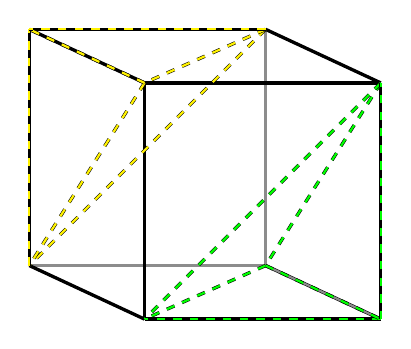
\begin{tikzpicture}[vertexStyle, edgeDouble, faceStyle, scale=1.5]
\draw [edge] (0.024390243902439324,1.4536585365853658)-- (2.024390243902439,1.4536585365853658);
\draw [edge] (2.024390243902439,1.4536585365853658)-- (2.024390243902439,3.453658536585366);
\draw [edge] (3,1)-- (2.024390243902439,1.4536585365853658);
\draw [edge=black] (1,1)-- (3,1);
\draw [edge=black] (3,1)-- (3,3);
\draw [edge=black] (3,3)-- (1,3);
\draw [edge=black] (1,3)-- (1,1);
\draw [edge=black] (0.024390243902439324,3.453658536585366)-- (0.024390243902439324,1.4536585365853658);
\draw [edge=black] (2.024390243902439,3.453658536585366)-- (0.024390243902439324,3.453658536585366);
\draw [edge=black] (1,3)-- (0.024390243902439324,3.453658536585366);
\draw [edge=black] (3,3)-- (2.024390243902439,3.453658536585366);
\draw [edge=black] (1,1)-- (0.024390243902439324,1.4536585365853658);
\draw [dashed, edge=green] (3,3)-- (2.024390243902439,1.4536585365853658);
\draw [dashed, edge=green] (2.024390243902439,1.4536585365853658)-- (1,1);
\draw [dashed, edge=green] (3,3)-- (1,1);
\draw [dashed, edge=green] (3,1)-- (1,1);
\draw [dashed, edge=green] (3,1)-- (3,3);
\draw [dashed, edge=green] (2.024390243902439,1.4536585365853658)-- (3,1);
\draw [dashed,edge=yellow] (2.024390243902439,3.453658536585366)-- (0.024390243902439324,1.4536585365853658);
\draw [dashed,edge=yellow] (2.024390243902439,3.453658536585366)-- (1,3);
\draw [dashed,edge=yellow] (1,3)-- (0.024390243902439324,1.4536585365853658);
\draw [dashed,edge=yellow] (1,3)-- (0.024390243902439324,3.453658536585366);
\draw [dashed,edge=yellow] (0.024390243902439324,1.4536585365853658)-- (0.024390243902439324,3.453658536585366);
\draw [dashed,edge=yellow] (2.024390243902439,3.453658536585366)-- (0.024390243902439324,3.453658536585366);
\end{tikzpicture}



\end{center}
 
\begin{Verbatim}[commandchars=!@|,fontsize=\small,frame=single,label=Example]
  !gapprompt@gap>| !gapinput@PE:=Cube()|
  polygonal surface ( 8 vertices, 12 edges, 6 faces)
  !gapprompt@gap>| !gapinput@VerticesOfFaces(PE);|
  [ [ 1, 2, 3, 4 ], [ 1, 2, 5, 6 ], [ 2, 3, 6, 7 ], [ 1, 4, 5, 8 ]
  [ 3, 4, 7, 8 ], [ 5, 6, 7, 8 ] ]
\end{Verbatim}
 

 There are two disjoint tetrahedra contained in this cube with the following
property: Each tetrahedron's faces subdivide three faces of the cube and the
tetrahedron's vertices are also vertices of the cube. 

 How can we find them? First we list each vertex together with its neighbour
vertices, so that we can find a pair of disjoint sets among them: 

 
\begin{Verbatim}[commandchars=!@|,fontsize=\small,frame=single,label=Example]
  !gapprompt@gap>| !gapinput@List([1..8], i-> NeighbourVerticesOfVertex(PE,i));|
  [ [ 2, 4, 5 ], [ 1, 3, 6 ], [ 2, 4, 7 ], [ 3, 1, 8 ], [ 1, 8, 6 ], 
   [ 2, 7, 5 ], [ 3, 6, 8 ], [ 4, 7, 5 ] ]
  !gapprompt@gap>| !gapinput@SS:=List([1..8], i->Union([i],last[i]));|
  [ [ 1, 2, 4, 5 ], [ 1, 2, 3, 6 ], [ 2, 3, 4, 7 ], [ 1, 3, 4, 8 ], 
   [ 1, 5, 6, 8 ], [ 2, 5, 6, 7 ], [ 3, 6, 7, 8 ], [ 4, 5, 7, 8 ] ]                                                ^
  !gapprompt@gap>| !gapinput@Filtered([1..8],i->Intersection(SS[1],SS[i])=[]);|
  [ 7 ]
  !gapprompt@gap>| !gapinput@T1:=SS[1]; T2:=SS[7];|
  [ 1, 2, 4, 5 ]
  [ 3, 6, 7, 8 ]
\end{Verbatim}
 

 Construct the corresponding tetrahedra: 

 
\begin{Verbatim}[commandchars=!@|,fontsize=\small,frame=single,label=Example]
  !gapprompt@gap>| !gapinput@Combinations(T1,3);|
  [ [ 1, 2, 4 ], [ 1, 2, 5 ], [ 1, 4, 5 ],[ 2, 4, 5]];
  !gapprompt@gap>| !gapinput@T1:=SimplicialSurfaceByVerticesInFaces(last);|
  simplicial surface (4 vertices, 6 edges, 4  faces)                
  
  !gapprompt@gap>| !gapinput@Combinations(T2,3);|
  [ [ 3, 6, 7 ], [ 3, 6, 8 ], [ 3, 6, 8 ], [ 6, 7, 8 ] ]
  !gapprompt@gap>| !gapinput@T1:=SimplicialSurfaceByVerticesInFaces(last);|
  simplicial surface (4 vertices, 6 edges, 4  faces) 
\end{Verbatim}
 

 
\begin{center}
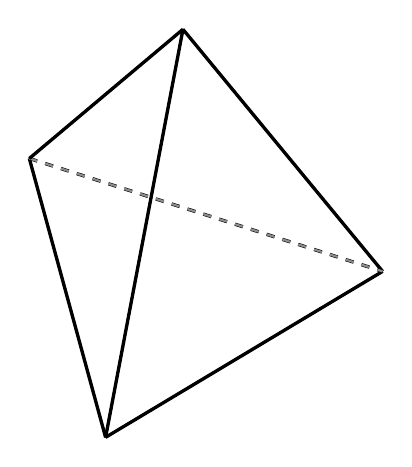
\begin{tikzpicture}[vertexBall, edgeDouble, faceStyle, scale=1]

\draw [edge=black] (-1.0314641277190677,-1.541558122060108)-- (2.4862868481518334,0.5659233184391239);
\draw [edge=black] (2.4862868481518334,0.5659233184391239)-- (-0.04902917049386102,3.639993991047026);
\draw [edge=black] (-0.04902917049386102,3.639993991047026)-- (-1.0314641277190677,-1.541558122060108);
\draw [edge=black] (-2,2)-- (-1.0314641277190677,-1.541558122060108);
\draw [dashed,edge] (-2,2)-- (2.4862868481518334,0.5659233184391239);
\draw [edge=black] (-2,2)-- (-0.04902917049386102,3.639993991047026);

\end{tikzpicture}

\end{center}
 

 Before proceeding with further computations, verify that the two simplcial
surfaces constructed are indeed isomorphic to the tetrahedron. 

 
\begin{Verbatim}[commandchars=!@|,fontsize=\small,frame=single,label=Example]
  !gapprompt@gap>| !gapinput@IsIsomorphic(T1,Tetrahedron());|
  true
  !gapprompt@gap>| !gapinput@IsIsomorphic(T2,Tetrahedron());|
  true
\end{Verbatim}
 

 Now use the edges of the tetrahedra T1 and T2 to subdivide the cube's faces.
More precisely take the edges of T1 and T2 not containing vertex 1 resp. 7 as
diagonals of the faces of PE in which they lie to subdivide each of these
faces into two triangular faces: 

 
\begin{Verbatim}[commandchars=!@|,fontsize=\small,frame=single,label=Example]
  !gapprompt@gap>| !gapinput@ VerticesOfFaces(PE);|
  [ [ 1, 2, 3, 4 ], [ 1, 2, 5, 6 ], [ 2, 3, 6, 7 ], [ 1, 4, 5, 8 ], 
    [ 3, 4, 7, 8 ], [ 5, 6, 7, 8 ] ]
  !gapprompt@gap>| !gapinput@VerticesOfEdges(T1);|
  [ [ 1, 2 ], [ 1, 4 ], [ 1, 5 ], [ 2, 4 ], [ 2, 5 ], [ 4, 5 ] ]
  !gapprompt@gap>| !gapinput@VerticesOfEdges(T2);|
  [ [ 3, 6 ], [ 3, 7 ], [ 3, 8 ], [ 6, 7 ], [ 6, 8 ], [ 7, 8 ] ]
  !gapprompt@gap>| !gapinput@neEd:= Union(Filtered(VerticesOfEdges(T1),r->not 1 in|
  !gapprompt@>| !gapinput@r),Filtered(VerticesOfEdges(T2),r->not 7 in r));|
  [ [ 2, 4 ], [ 2, 5 ], [ 3, 6 ], [ 3, 8 ], [ 4, 5 ], [ 6, 8 ] ]
  
  !gapprompt@gap>| !gapinput@neEd:=List(VerticesOfFaces(PE), r->Filtered(neEd,s->IsSubset(r,s))[1]);|
  [ [ 2, 4 ], [ 2, 5 ], [ 3, 6 ], [ 4, 5 ], [ 3, 8 ], [ 6, 8 ] ]
  !gapprompt@gap>| !gapinput@List([1..6], i->IsSubset(VerticesOfFaces(PE)[i],neEd[i]));|
  [ true, true, true, true, true, true ]
\end{Verbatim}
 

 
\begin{center}


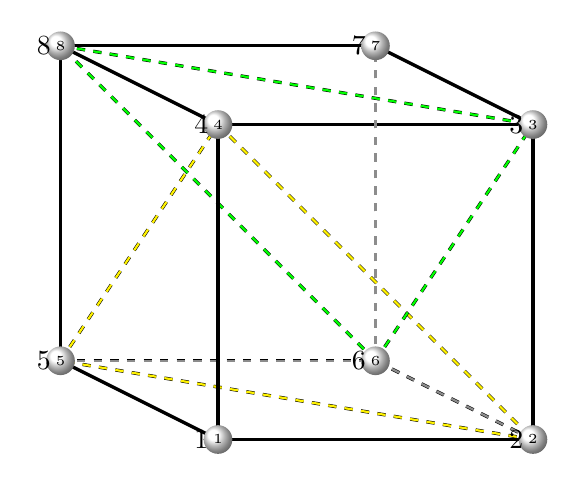
\begin{tikzpicture}[vertexBall, edgeDouble, faceStyle, scale=1]

% Define the coordinates of the vertices
\coordinate (V1_1) at (0, 0);
\coordinate (V2_1) at (4, 0);
\coordinate (V3_1) at (4,4);
\coordinate (V4_1) at (0,4);
\coordinate (V5_1) at (-2,1);
\coordinate (V6_1) at (2,1);
\coordinate (V7_1) at (2,5);
\coordinate (V8_1) at (-2,5);

\draw [edge=black] (0,0)-- (4,0);
\draw [edge=black] (4,0)-- (4,4);
\draw [edge=black] (4,4)-- (0,4);
\draw [edge=black] (-2,5)-- (-2,1);
\draw [dashed, edge] (-2,1)-- (2,1);
\draw [dashed, edge] (2,1)-- (2,5);
\draw [edge=black] (2,5)-- (-2,5);
\draw [edge=black] (0,0)-- (-2,1);
\draw [dashed, edge] (4,0)-- (2,1);
\draw [edge=black] (4,4)-- (2,5);
\draw [edge=black] (0,4)-- (-2,5);
\draw [dashed, edge=green] (-2,5)-- (4,4);
\draw [dashed, edge=yellow] (0,4)-- (4,0);
\draw [dashed, edge=yellow] (4,0)-- (-2,1);
\draw [dashed, edge=yellow] (-2,1)-- (0,4);
\draw [dashed, edge=green] (2,1)-- (4,4);
\draw [dashed, edge=green] (2,1)-- (-2,5);
\draw [edge=black] (0,4)-- (0,0);
\vertexLabelR{V1_1}{left}{$1$}
\vertexLabelR{V2_1}{left}{$2$}
\vertexLabelR{V3_1}{left}{$3$}
\vertexLabelR{V4_1}{left}{$4$}
\vertexLabelR{V5_1}{left}{$5$}
\vertexLabelR{V6_1}{left}{$6$}
\vertexLabelR{V7_1}{left}{$7$}
\vertexLabelR{V8_1}{left}{$8$}

\end{tikzpicture}



\end{center}
 Now use the set \texttt{neEd} defined above to subdivide the cube's faces with the following function: 

 
\begin{Verbatim}[commandchars=!@|,fontsize=\small,frame=single,label=Example]
  !gapprompt@gap>| !gapinput@part:=function(Q,E)|
  # Q set of vertices of old faces 
  # E diagonal Edges
  !gapprompt@>| !gapinput@local ne;|
  !gapprompt@>| !gapinput@ne:=Difference(Q,E); |
  !gapprompt@>| !gapinput@return [Union(E,[ne[1]]),Union(E,[ne[2]])];|
  !gapprompt@>| !gapinput@end;|
  function( Q, E ) ... end
\end{Verbatim}
 

 Construct the simplicial parallelepiped by defining the faces represented by
their sets of vertices. Note, this works only because the parallelepiped is
vertex-faithful. 

 
\begin{Verbatim}[commandchars=!@|,fontsize=\small,frame=single,label=Example]
  !gapprompt@gap>| !gapinput@List([1..6],i->part(VerticesOfFaces(PE)[i],neEd[i]));|
  [ [ [ 1, 2, 4 ], [ 2 .. 4 ] ], [ [ 1, 2, 5 ], [ 2, 5, 6 ] ],
   [ [ 2, 3, 6 ], [ 3, 6, 7 ] ], [ [ 1, 4, 5 ], [ 4, 5, 8 ] ], 
   [ [ 3, 4, 8 ], [ 3, 7, 8 ] ], [ [ 5, 6, 8 ], [ 6 .. 8 ] ] ]
  
  !gapprompt@gap>| !gapinput@Union(last);|
  [ [ 1, 2, 4 ], [ 1, 2, 5 ], [ 1, 4, 5 ], [ 2 .. 4 ], [ 2, 3, 6 ],
   [ 2, 5, 6 ], [ 3, 4, 8 ], [ 3, 6, 7 ], [ 3, 7, 8 ], [ 4, 5, 8 ], 
   [ 5, 6, 8 ], [ 6 .. 8 ] ]
  
  !gapprompt@gap>| !gapinput@PE:=SimplicialSurfaceByVerticesInFaces(last);|
  simplicial surface ( 8 vertices, 18 edges, 12 faces )
\end{Verbatim}
 

 We show that the surface has Euler characteristic 2 and vertex counter $v_3^2 v_5^6$. 

 
\begin{Verbatim}[commandchars=!@|,fontsize=\small,frame=single,label=Example]
  !gapprompt@gap>| !gapinput@EulerCharacteristic(PE);|
  2
  !gapprompt@gap>| !gapinput@FacesOfVertices(PE);|
  [ [ 1, 2, 3 ], [ 1, 2, 4, 5, 6 ], [ 4, 5, 7, 8, 9 ], [ 1, 3, 4, 7, 10 ],
    [ 2, 3, 6, 10, 11 ], [ 5, 6, 8, 11, 12 ], [ 8, 9, 12 ],
   [ 7, 9, 10, 11, 12 ] ];
  !gapprompt@gap>| !gapinput@VertexCounter(PE);|
  [ [ 3, 2 ], [ 5, 6 ] ]
\end{Verbatim}
 

 Computing the set of vertices connected to a given vertex via an edge with the
command \texttt{NeighbourVerticesOfVertex} 

 
\begin{Verbatim}[commandchars=!@|,fontsize=\small,frame=single,label=Example]
  !gapprompt@gap>| !gapinput@NeighbourVerticesOfVertex(PE,1);|
  [ 2, 4, 5 ]
  !gapprompt@gap>| !gapinput@NeighbourVerticesOfVertex(PE,2);NeighbourVerticesOfVertex(PE,4);|
  [ 1, 3, 4, 5, 6 ]
  [ 1, 2, 3, 5, 8 ]
  !gapprompt@gap>| !gapinput@NeighbourVerticesOfVertex(PE,7);|
  [ 3, 6, 8 ]
\end{Verbatim}
 

 Therefore we see that the simplicial surface \texttt{PE} is a sphere with the following umbrella descriptor. 

 
\begin{Verbatim}[commandchars=!@|,fontsize=\small,frame=single,label=Example]
  !gapprompt@gap>| !gapinput@List(UmbrellaPathsOfVertices(PE),r->FacesAsPerm(r));|
  [ (1,3,2), (1,4,5,6,2), (4,7,9,8,5), (1,4,7,10,3), (2,6,11,10,3),
  (5,8,12,11,6), (8,12,9), (7,10,11,12,9) ]
\end{Verbatim}
 

 }

 
\subsection{\textcolor{Chapter }{Construction from an octahedron}}\label{Chapter_Tutorial_Section_Parallelelepiped_Subsection_Construction_from_an_octahedron}
\logpage{[ 3, 1, 2 ]}
\hyperdef{L}{X8079D1687A5047B4}{}
{
  

 $Idea$ $behind$ $the$ $construcion$ 

 We want to construct the simplicial parallelepiped using tetrahedrial
extensions. Starting from an octahedron we subdivide two disjoint faces into
3-gons, whereby the faces of the surfaces are represented by their sets of
vertices. Subdividing a face of a simplicial surface gives rise to a new
surface which can be seen as subdivision of the given surface. 

 
\begin{center}
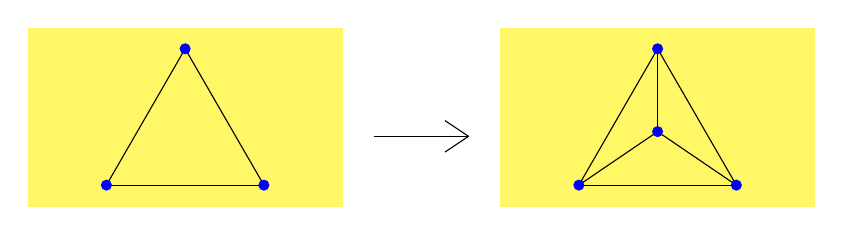
\begin{tikzpicture}[vertexBall, edgeDouble, faceStyle, scale=2, edgeStyle=nolabels,vertexStyle=nolabels]
\coordinate (V1) at (-1.5, 0.8660254037844386);
\coordinate (V2) at (-1, 0);
\coordinate (V3) at (-2, 0);
\coordinate (V4) at (1.5, 0.8660254037844386);
\coordinate (V5) at (1, 0);
\coordinate (V6) at (2, 0);
\coordinate (V7) at (1.5, 0.34);

\fill[face]  (0.5,-0.14) -- (2.5,-0.14) -- (2.5,1) -- (0.5,1) -- cycle;
\fill[face]  (-0.5,-0.14) -- (-2.5,-0.14) -- (-2.5,1) -- (-0.5,1) -- cycle;

\draw[edge=black] (-0.3,0.31) -- (0.3,0.31);
\draw[edge=black] (0.15,0.41) -- (0.3,0.31);
\draw[edge=black] (0.15,0.21) -- (0.3,0.31);
\draw[edge=black] (V1) -- (V2);
\draw[edge=black] (V2) -- (V3);
\draw[edge=black] (V1) -- (V3);
\draw[edge=black] (V4) -- (V5);
\draw[edge=black] (V5) -- (V6);
\draw[edge=black] (V4) -- (V6);
\draw[edge=black] (V4) -- (V7);
\draw[edge=black] (V5) -- (V7);
\draw[edge=black] (V6) -- (V7);

\vertexLabelR{V1}{left}{}
\vertexLabelR{V2}{left}{}
\vertexLabelR{V3}{left}{}
\vertexLabelR{V4}{left}{}
\vertexLabelR{V5}{left}{}
\vertexLabelR{V6}{left}{}
\vertexLabelR{V7}{left}{}
\end{tikzpicture}

\end{center}
 
\begin{Verbatim}[commandchars=!@|,fontsize=\small,frame=single,label=Example]
  !gapprompt@gap>| !gapinput@O1:=Octahedron();|
  simplicial surface ( 6 vertices, 12 edges, 8 faces )
  
  !gapprompt@gap>| !gapinput@VO1:=VerticesOfFaces(O1);|
  [ [ 1, 2, 3 ], [ 2, 5, 6 ], [ 1, 2, 5 ], [ 2, 3, 6 ], [ 1, 4, 5 ],
   [ 3, 4, 6 ], [ 1, 3, 4 ], [ 4, 5, 6 ] ]
\end{Verbatim}
 

 Determine the faces which will be replaced by attaching the tetrahedra.
Therefore search for two faces that share no common vertex. 

 
\begin{Verbatim}[commandchars=!@|,fontsize=\small,frame=single,label=Example]
  !gapprompt@gap>| !gapinput@Filtered(VO1,r->Intersection(VO1[1],r)=[]);|
  [ [ 4, 5, 6 ] ]
\end{Verbatim}
 

 
\begin{center}

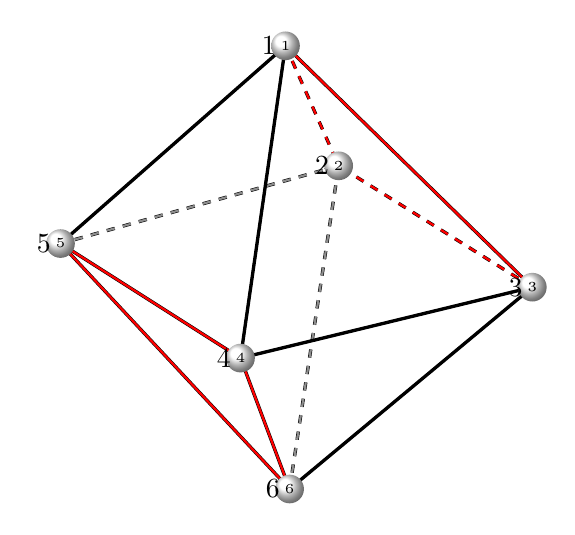
\begin{tikzpicture}[vertexBall, edgeDouble, faceStyle, scale=1]
\coordinate (V1_1) at (-0.07029763931478862,2.758422481241498);
\coordinate (V2_1) at (0.6051024855158862,1.2344427123927926);
\coordinate (V3_1) at (3.064251657976292,-0.3068550083746484);
\coordinate (V4_1) at (-0.641790052633052,-1.2073885081488835);
\coordinate (V5_1) at (-2.927759705906105,0.2473194530248809);
\coordinate (V6_1) at (-0.01834378355858286,-2.8699118923474716);

\draw [dashed,edge= red] (-0.07029763931478862,2.758422481241498)-- (0.6051024855158862,1.2344427123927926);
\draw [dashed, edge] (-0.01834378355858286,-2.8699118923474716)-- (0.6051024855158862,1.2344427123927926);
\draw [dashed, edge] (0.6051024855158862,1.2344427123927926)-- (-2.927759705906105,0.2473194530248809);
\draw [dashed,edge=red] (3.064251657976292,-0.3068550083746484)-- (0.6051024855158862,1.2344427123927926);
\draw [edge=red] (-2.927759705906105,0.2473194530248809)-- (-0.641790052633052,-1.2073885081488835);
\draw [edge=red] (-0.01834378355858286,-2.8699118923474716)-- (-2.927759705906105,0.2473194530248809);

\draw [edge=black] (-0.07029763931478862,2.758422481241498)-- (-2.927759705906105,0.2473194530248809);
\draw [edge=red] (-0.07029763931478862,2.758422481241498)-- (3.064251657976292,-0.3068550083746484);
\draw [edge=black] (3.064251657976292,-0.3068550083746484)-- (-0.641790052633052,-1.2073885081488835);
\draw [edge=black] (-0.641790052633052,-1.2073885081488835)-- (-0.07029763931478862,2.758422481241498);
\draw [edge=red] (-0.641790052633052,-1.2073885081488835)-- (-0.01834378355858286,-2.8699118923474716);
\draw [edge=black] (-0.01834378355858286,-2.8699118923474716)-- (3.064251657976292,-0.3068550083746484);

\vertexLabelR{V1_1}{left}{$1$}
\vertexLabelR{V2_1}{left}{$2$}
\vertexLabelR{V3_1}{left}{$3$}
\vertexLabelR{V4_1}{left}{$4$}
\vertexLabelR{V5_1}{left}{$5$}
\vertexLabelR{V6_1}{left}{$6$}

\end{tikzpicture}


\end{center}
 

 Compute the tetrahedra's vertices of faces so that the octahedron and each
tetrahedron have exactly three vertices in common. 

 
\begin{Verbatim}[commandchars=!@|,fontsize=\small,frame=single,label=Example]
  !gapprompt@gap>| !gapinput@FT1:=Combinations([1,2,3,7],3);|
  [ [ 1, 2, 3 ], [ 1, 2, 7 ], [ 1, 3, 7 ], [ 2, 3, 7 ] ]
  !gapprompt@gap>| !gapinput@FT2:=Combinations([4,5,6,8],3);|
  [ [ 4, 5, 6 ], [ 4, 5, 8 ], [ 4, 6, 8 ], [ 5, 6, 8 ] ]
\end{Verbatim}
 

 Define the symmetric difference \texttt{sydif()} of sets A and B 

 
\begin{Verbatim}[commandchars=!@|,fontsize=\small,frame=single,label=Example]
  !gapprompt@gap>| !gapinput@symdif:=function(A,B)|
  !gapprompt@>| !gapinput@return Difference(Union(A,B),Intersection(A,B));|
  !gapprompt@>| !gapinput@end;|
  function( A, B ) ... end
\end{Verbatim}
 

 Why is the symmetric difference helpful for the solution of this problem? 

 The symmetric difference of the set of faces of the octahedron and the set of
faces of one of the above tetrahedra removes the face \texttt{[1,2,3]} resp. \texttt{[4,5,6]} which the octahedron and the tetrahedron have in common and replaces it with
the three remaining faces of the tetrahedron. So by using the symmetric
difference we obtain the vertices of faces of the desired simplicial
parallelepiped. 

 
\begin{Verbatim}[commandchars=!@|,fontsize=\small,frame=single,label=Example]
  !gapprompt@gap>| !gapinput@symdif(VO1,FT1);|
  [ [ 1, 2, 5 ], [ 1, 2, 7 ], [ 1, 3, 4 ], [ 1, 3, 7 ], [ 1, 4, 5 ],
  [ 2, 3, 6 ], [ 2, 3, 7 ], [ 2, 5, 6 ], [ 3, 4, 6 ], [ 4, 5, 6 ] ]
  !gapprompt@gap>| !gapinput@symdif(last,FT2);|
  [ [ 1, 2, 5 ], [ 1, 2, 7 ], [ 1, 3, 4 ], [ 1, 3, 7 ], [ 1, 4, 5 ],
   [ 2, 3, 6 ], [ 2, 3, 7 ], [ 2, 5, 6 ], [ 3, 4, 6 ], [ 4, 5, 8 ],
   [ 4, 6, 8 ], [ 5, 6, 8 ] ]
\end{Verbatim}
 

 Finally construct the simplicial parallelepiped 

 
\begin{Verbatim}[commandchars=!@|,fontsize=\small,frame=single,label=Example]
  !gapprompt@gap>| !gapinput@PEn:=SimplicialSurfaceByVerticesInFaces(last);|
  simplicial surface ( vertices, 18 edges, 12 faces )
\end{Verbatim}
 
\begin{center}
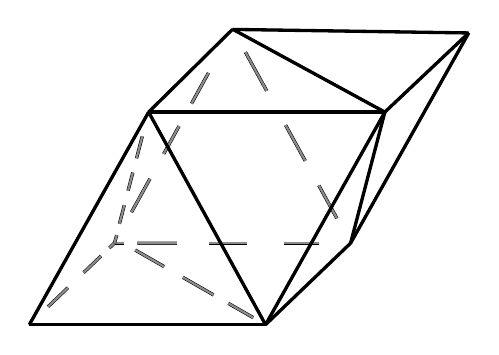
\begin{tikzpicture}[vertexBall, edgeDouble, faceStyle, scale=0.75]

\draw [edge=black] (-2,0)-- (2,0);

\draw [edge=black] (4.02,3.6)-- (0.02,3.6);
\draw [edge=black] (0.02,3.6)-- (-2,0);
\draw [edge=black] (3.44,1.38)-- (5.44,4.94);
\draw [edge=black] (5.44,4.94)-- (1.44,5);
\draw [edge=black] (2,0)-- (3.44,1.38);
\draw [edge=black] (1.44,5)-- (0.02,3.6);
\draw [edge=black] (4.02,3.6)-- (5.44,4.94);
\draw [edge] (1.0332274736325155,4.263741727274853)-- (0.7467514791515633,3.7452201772643297);
\draw [edge] (0.5353438881223546,3.362572437501462)-- (0.27515352774724633,2.891627885222516);
\draw [edge] (0.04213746170575994,2.4698688056874256)-- (-0.2706241668810365,1.903770257945324);
\draw [edge] (-0.17237103195467773,1.380053770842896)-- (0.5,1.38);
\draw [edge] (1.04,1.38)-- (1.68,1.38);
\draw [edge] (2.32,1.38)-- (2.9,1.38);
\draw [edge] (-0.7850135746606335,1.1643619909502263)-- (-1.0803981900452488,0.8812850678733032);
\draw [edge] (-1.3462443438914027,0.6265158371040724)-- (-1.68289592760181,0.303891402714932);
\draw [edge=black] (1.445708891887561,5.001217790538086)-- (4.02,3.6);
\draw [edge=black] (4.02,3.6)-- (3.44,1.38);
\draw [edge] (-0.20657687221433152,1.2634432090904641)-- (0.28208649654699514,0.9836440221384141);
\draw [edge] (0.6006954988489983,0.801214674046138)-- (1.1194827839545476,0.5041671156389285);
\draw [edge] (1.3693663636853701,0.3610886143414413)-- (1.7904098214480486,0.12000727965474631);
\draw [edge] (1.6586800662532202,4.614506441153063)-- (2.0193178570905728,3.9596632345578975);
\draw [edge] (2.3391022653831035,3.3790012721517955)-- (2.672007457959911,2.7745146949325603);
\draw [edge] (2.901332820391631,2.35810754209451)-- (3.209287291452826,1.7989262847814618);
\draw [edge] (-0.08740460161040448,3.1888996283187967)-- (-0.18448630955407658,2.817311022051638);
\draw [edge] (-0.24757816479935152,2.57582150714731)-- (-0.327664946393825,2.2692824465615664);
\draw [edge] (-0.47394672494161083,1.7093763286717656)-- (-0.39168935199695565,2.024223514770273);
\draw [edge] (-0.56,1.38)-- (-0.4,1.38);
\draw [edge] (-0.56,1.38)-- (-0.6456793566202854,1.2978906165722264);
\draw [edge] (-0.56,1.38)-- (-0.5195862057533234,1.5160463805806987);
\draw [edge=black] (2,0)-- (0.02,3.6);
\draw [edge=black] (2,0)-- (4.02,3.6);

\end{tikzpicture}



\end{center}
 

 If the first and second construction were carried out correctly, the
constructed simplicial surfaces must be isomorphic. 

 
\begin{Verbatim}[commandchars=!@|,fontsize=\small,frame=single,label=Example]
  !gapprompt@gap>| !gapinput@IsIsomorphic(PE,PEn);|
  true
\end{Verbatim}
 }

 
\subsection{\textcolor{Chapter }{Construction from an octahedron (2)}}\label{Chapter_Tutorial_Section_Parallelelepiped_Subsection_Construction_from_an_octahedron_2}
\logpage{[ 3, 1, 3 ]}
\hyperdef{L}{X843C6E4E7DB83B98}{}
{
  

 $Idea$ $behind$ $the$ $construcion$ 

 As seen in the previous construction two tetrahedra can be attached to an
octahedron to construct the simplical parallelepiped. In this subsection we
present an alternative construction. The required simplicial surfaces are
computed directly instead of manipulating their vertices in faces to create
the simplicial parallelepiped. This is achieved by using flags. A flag is a
triple [ V, E, F ] satisfying the following conditions: 
\begin{itemize}
\item  the vertex V is incident to the edge E 
\item  the edge E is incident to the face F 
\item  the vertex V is incident to the face F. 
\end{itemize}
 

 We can compute flags by calling 
\begin{Verbatim}[commandchars=!@|,fontsize=\small,frame=single,label=Example]
  !gapprompt@gap>| !gapinput@Flags(Tetrahedron());|
  [ [ 1, 1, 1 ], [ 1, 1, 2 ], [ 1, 2, 1 ], [ 1, 2, 4 ], [ 1, 3, 2 ], 
   [ 1, 3, 4 ], [ 2, 1, 1 ], [ 2, 1, 2 ], [ 2, 4, 1 ], [ 2, 4, 3 ], 
   [ 2, 5, 2 ], [ 2, 5, 3 ], [ 3, 2, 1 ], [ 3, 2, 4 ], [ 3, 4, 1 ], 
   [ 3, 4, 3 ], [ 3, 6, 3 ], [ 3, 6, 4 ], [ 4, 3, 2 ], [ 4, 3, 4 ], 
   [ 4, 5, 2 ], [ 4, 5, 3 ], [ 4, 6, 3 ], [ 4, 6, 4 ] ]
\end{Verbatim}
 

 Use these flags to attach the tetrahedron to the octahedron with the function \texttt{ConnectedFaceSum()} 

 
\begin{Verbatim}[commandchars=!@|,fontsize=\small,frame=single,label=Example]
  !gapprompt@gap>| !gapinput@PE3:=ConnectedFaceSum(Tetrahedron(),[1,1,1],Octahedron(),[1,1,1]);|
  [simplicial surface (7 vertices, 15 edges, 10 faces)]
\end{Verbatim}
 

 
\begin{center}
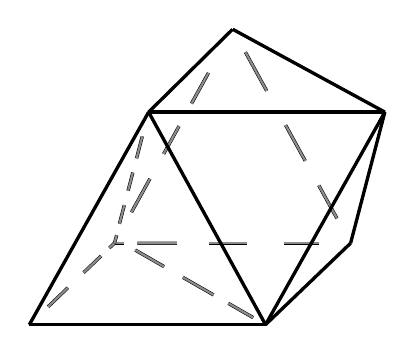
\begin{tikzpicture}[vertexBall, edgeDouble, faceStyle, scale=0.75]

\draw [edge=black] (-2,0)-- (2,0);

\draw [edge=black] (4.02,3.6)-- (0.02,3.6);
\draw [edge=black] (0.02,3.6)-- (-2,0);
%\draw [edge=black] (3.44,1.38)-- (5.44,4.94);
%\draw [edge=black] (5.44,4.94)-- (1.44,5);
\draw [edge=black] (2,0)-- (3.44,1.38);
\draw [edge=black] (1.44,5)-- (0.02,3.6);
%\draw [edge=black] (4.02,3.6)-- (5.44,4.94);
\draw [edge] (1.0332274736325155,4.263741727274853)-- (0.7467514791515633,3.7452201772643297);
\draw [edge] (0.5353438881223546,3.362572437501462)-- (0.27515352774724633,2.891627885222516);
\draw [edge] (0.04213746170575994,2.4698688056874256)-- (-0.2706241668810365,1.903770257945324);
\draw [edge] (-0.17237103195467773,1.380053770842896)-- (0.5,1.38);
\draw [edge] (1.04,1.38)-- (1.68,1.38);
\draw [edge] (2.32,1.38)-- (2.9,1.38);
\draw [edge] (-0.7850135746606335,1.1643619909502263)-- (-1.0803981900452488,0.8812850678733032);
\draw [edge] (-1.3462443438914027,0.6265158371040724)-- (-1.68289592760181,0.303891402714932);
\draw [edge=black] (1.445708891887561,5.001217790538086)-- (4.02,3.6);
\draw [edge=black] (4.02,3.6)-- (3.44,1.38);
\draw [edge] (-0.20657687221433152,1.2634432090904641)-- (0.28208649654699514,0.9836440221384141);
\draw [edge] (0.6006954988489983,0.801214674046138)-- (1.1194827839545476,0.5041671156389285);
\draw [edge] (1.3693663636853701,0.3610886143414413)-- (1.7904098214480486,0.12000727965474631);
\draw [edge] (1.6586800662532202,4.614506441153063)-- (2.0193178570905728,3.9596632345578975);
\draw [edge] (2.3391022653831035,3.3790012721517955)-- (2.672007457959911,2.7745146949325603);
\draw [edge] (2.901332820391631,2.35810754209451)-- (3.209287291452826,1.7989262847814618);
\draw [edge] (-0.08740460161040448,3.1888996283187967)-- (-0.18448630955407658,2.817311022051638);
\draw [edge] (-0.24757816479935152,2.57582150714731)-- (-0.327664946393825,2.2692824465615664);
\draw [edge] (-0.47394672494161083,1.7093763286717656)-- (-0.39168935199695565,2.024223514770273);
\draw [edge] (-0.56,1.38)-- (-0.4,1.38);
\draw [edge] (-0.56,1.38)-- (-0.6456793566202854,1.2978906165722264);
\draw [edge] (-0.56,1.38)-- (-0.5195862057533234,1.5160463805806987);
\draw [edge=black] (2,0)-- (0.02,3.6);
\draw [edge=black] (2,0)-- (4.02,3.6);
\end{tikzpicture}



\end{center}
 

 We have to find the face which has to be replaced by the second tetrahedron.
How do we find it? The vertices of this face are not incident to the already
attached tetrahedron, thus their face degree must be 4. 

 
\begin{Verbatim}[commandchars=!@|,fontsize=\small,frame=single,label=Example]
  !gapprompt@gap>| !gapinput@FaceDegreesOfVertices(PE3);|
  [ ,,, 3,,,,,, 4, 4, 4, 5, 5, 5 ]
  !gapprompt@gap>| !gapinput@Vertices(PE3);|
  [ 4, 10, 11, 12, 13, 14, 15 ]
  !gapprompt@gap>| !gapinput@Intersection(List([10,11,12],i->FacesOfVertex(PE3,i)));|
  [ 14 ]
\end{Verbatim}
 

 Find the edge E of the corresponding flag \texttt{[10, E, 14]} to compute the simplicial parallelepiped 

 
\begin{Verbatim}[commandchars=!@|,fontsize=\small,frame=single,label=Example]
  !gapprompt@gap>| !gapinput@Intersection(EdgesOfFace(PE3,14),EdgesOfVertex(PE3,10));|
  [ 16, 17 ]
  !gapprompt@gap>| !gapinput@PE3:=ConnectedFaceSum(Tetrahedron(),[1,1,1],PE3,[10,16,14]);|
  simplicial surface (8 vertices, 18 edges, 12 faces)
\end{Verbatim}
 

 
\begin{center}
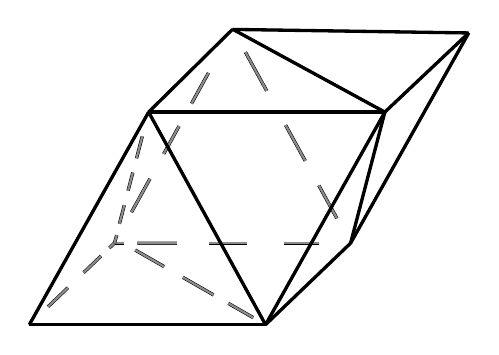
\begin{tikzpicture}[vertexBall, edgeDouble, faceStyle, scale=0.75]

\draw [edge=black] (-2,0)-- (2,0);

\draw [edge=black] (4.02,3.6)-- (0.02,3.6);
\draw [edge=black] (0.02,3.6)-- (-2,0);
\draw [edge=black] (3.44,1.38)-- (5.44,4.94);
\draw [edge=black] (5.44,4.94)-- (1.44,5);
\draw [edge=black] (2,0)-- (3.44,1.38);
\draw [edge=black] (1.44,5)-- (0.02,3.6);
\draw [edge=black] (4.02,3.6)-- (5.44,4.94);
\draw [edge] (1.0332274736325155,4.263741727274853)-- (0.7467514791515633,3.7452201772643297);
\draw [edge] (0.5353438881223546,3.362572437501462)-- (0.27515352774724633,2.891627885222516);
\draw [edge] (0.04213746170575994,2.4698688056874256)-- (-0.2706241668810365,1.903770257945324);
\draw [edge] (-0.17237103195467773,1.380053770842896)-- (0.5,1.38);
\draw [edge] (1.04,1.38)-- (1.68,1.38);
\draw [edge] (2.32,1.38)-- (2.9,1.38);
\draw [edge] (-0.7850135746606335,1.1643619909502263)-- (-1.0803981900452488,0.8812850678733032);
\draw [edge] (-1.3462443438914027,0.6265158371040724)-- (-1.68289592760181,0.303891402714932);
\draw [edge=black] (1.445708891887561,5.001217790538086)-- (4.02,3.6);
\draw [edge=black] (4.02,3.6)-- (3.44,1.38);
\draw [edge] (-0.20657687221433152,1.2634432090904641)-- (0.28208649654699514,0.9836440221384141);
\draw [edge] (0.6006954988489983,0.801214674046138)-- (1.1194827839545476,0.5041671156389285);
\draw [edge] (1.3693663636853701,0.3610886143414413)-- (1.7904098214480486,0.12000727965474631);
\draw [edge] (1.6586800662532202,4.614506441153063)-- (2.0193178570905728,3.9596632345578975);
\draw [edge] (2.3391022653831035,3.3790012721517955)-- (2.672007457959911,2.7745146949325603);
\draw [edge] (2.901332820391631,2.35810754209451)-- (3.209287291452826,1.7989262847814618);
\draw [edge] (-0.08740460161040448,3.1888996283187967)-- (-0.18448630955407658,2.817311022051638);
\draw [edge] (-0.24757816479935152,2.57582150714731)-- (-0.327664946393825,2.2692824465615664);
\draw [edge] (-0.47394672494161083,1.7093763286717656)-- (-0.39168935199695565,2.024223514770273);
\draw [edge] (-0.56,1.38)-- (-0.4,1.38);
\draw [edge] (-0.56,1.38)-- (-0.6456793566202854,1.2978906165722264);
\draw [edge] (-0.56,1.38)-- (-0.5195862057533234,1.5160463805806987);
\draw [edge=black] (2,0)-- (0.02,3.6);
\draw [edge=black] (2,0)-- (4.02,3.6);

\end{tikzpicture}



\end{center}
 

 The vertex counter verifies that the constructed surface is indeed the
simplicial parallelepiped 

 
\begin{Verbatim}[commandchars=!@|,fontsize=\small,frame=single,label=Example]
  !gapprompt@gap>| !gapinput@VertexCounter(PE3);|
  [ [ 3, 2 ], [ 5, 6 ] ]
\end{Verbatim}
 

 The numbering of the vertices etc. can and should be improved in the sense
that 
\begin{itemize}
\item  the vertices of the surface are given by the set [1..8] 
\item  the edges of the surface are given by the set [1..18] 
\item  the faces of the surface are given by the set [1..12] 
\end{itemize}
 This can be achieved by mapping each vertex to their position in \texttt{Vertices(PE3)} 
\begin{Verbatim}[commandchars=!@|,fontsize=\small,frame=single,label=Example]
  !gapprompt@gap>| !gapinput@VV:=Vertices(PE3);|
  [ 4, 10, 19, 20, 21, 22, 23, 24 ]
  !gapprompt@gap>| !gapinput@LL:=VerticesOfFaces(PE3);|
  [ , [ 4, 22, 23 ], [ 4, 23, 24 ], [ 4, 22, 24 ],,,, [ 10, 19, 20 ], 
   [ 10, 20, 21 ], [ 10, 19, 21 ],,,, [ 20, 23, 24 ], [ 19, 20, 23 ], 
   [ 20, 21, 24 ], [ 19, 22, 23 ], [ 21, 22, 24 ], [ 19, 21, 22 ] ]
  !gapprompt@gap>| !gapinput@LL:=Set(LL);|
  [ [ 4, 22, 23 ], [ 4, 22, 24 ], [ 4, 23, 24 ], [ 10, 19, 20 ], 
   [ 10, 19, 21 ], [ 10, 20, 21 ], [ 19, 20, 23 ], [ 19, 21, 22 ], 
   [ 19, 22, 23 ], [ 20, 21, 24 ], [ 20, 23, 24 ], [ 21, 22, 24 ] ]
  !gapprompt@gap>| !gapinput@LL:=List(LL,r->List(r,i->Position(VV,i)));|
  [ [ 1, 6, 7 ], [ 1, 6, 8 ], [ 1, 7, 8 ], [ 2, 3, 4 ], [ 2, 3, 5 ], 
   [ 2, 4, 5 ], [ 3, 4, 7 ], [ 3, 5, 6 ], [ 3, 6, 7 ], [ 4, 5, 8 ], 
   [ 4, 7, 8 ], [ 5, 6, 8 ] ]
  !gapprompt@gap>| !gapinput@PE3:=SimplicialSurfaceByVerticesInFaces(LL);|
  simplicial surface ( 8 vertices, 18 edges, 12 faces)
  !gapprompt@gap>| !gapinput@Vertices(PE3);|
  [ 1, 2, 3, 4, 5, 6, 7, 8 ]
\end{Verbatim}
 

 Verify that the resulting sphere is still isomorphic to the parallelepiped 

 
\begin{Verbatim}[commandchars=!@|,fontsize=\small,frame=single,label=Example]
  !gapprompt@gap>| !gapinput@FaceDegreesOfVertices(PE3);|
  [ 3, 3, 5, 5, 5, 5, 5, 5 ]
  !gapprompt@gap>| !gapinput@IsIsomorphic(PE3, PEn);|
  true
\end{Verbatim}
 

 }

 
\subsection{\textcolor{Chapter }{Construction from double-6-gon via butterfly turning (1)}}\label{Chapter_Tutorial_Section_Parallelelepiped_Subsection_Construction_from_double-6-gon_via_butterfly_turning_1}
\logpage{[ 3, 1, 4 ]}
\hyperdef{L}{X8026D11B7D8E4A98}{}
{
  $idea$ $behind$ $the$ \texttt{construction} 

 This construction uses the concept of edge-turns. If an inner edge e gives
rise to a butterfly (e.g. if the surface is vertex faithful), a new surface
can be created by turning the inner edge e. This amounts to replacing e by a
new edge e' connecting the other two vertices of the butterfly. So it has the
same number of faces, edges and vertices, but the vertex degrees in four
positions will change by +-1 i.e. the vertex degrees of the vertices incidient
to e decrease and the degrees of the vertices incident to e' increase by 1. We
shall refer to the edge e' as the orthogonal edge. In this construction we
perform edge-turns on the double-6-gon to obtain the simplicial
parallelepiped. 
\begin{center}

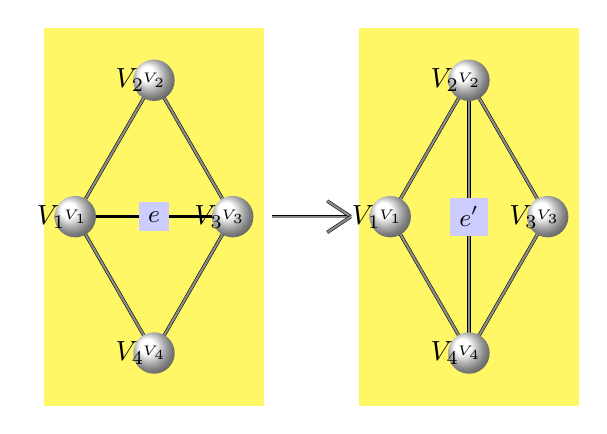
\begin{tikzpicture}[vertexBall, edgeDouble, faceStyle, scale=2]

% Define the coordinates of the vertices
\coordinate (V1_1) at (0, 0);
\coordinate (V2_1) at (1, 0);
\coordinate (V3_1) at (0.4999999999999999, 0.8660254037844386);
\coordinate (V4_1) at (0.4999999999999999, -0.8660254037844386);

\coordinate (V1_2) at (2, 0);
\coordinate (V2_2) at (3, 0);
\coordinate (V3_2) at (2.4999999999999999, 0.8660254037844386);
\coordinate (V4_2) at (2.4999999999999999, -0.8660254037844386);

% Fill in the faces
\fill[face]  (V2_1) -- (V3_1) -- (V1_1) -- cycle;
\fill[face]  (-0.2,-1.2) -- (1.2,-1.2) -- (1.2,1.2) -- (-0.2,1.2) -- cycle;
\fill[face]  (1.8,-1.2) -- (3.2,-1.2) -- (3.2,1.2) -- (1.8,1.2) -- cycle;
%\node[faceLabel] at (barycentric cs:V2_1=1,V3_1=1,V1_1=1) {$F$};


% Draw the edges
\draw[edge=black] (V2_1) -- node[edgeLabel] {$e$} (V1_1);
\draw[edge] (V1_1) -- (V3_1);
\draw[edge] (V3_1) --  (V2_1);
\draw[edge] (V4_1) --  (V2_1);
\draw[edge] (V4_1) --  (V1_1);

\draw[edge] (V3_2) -- node[edgeLabel] {$e'$} (V4_2);
\draw[edge] (V1_2) --  (V3_2);
\draw[edge] (V3_2) --  (V2_2);
\draw[edge] (V4_2) --  (V2_2);
\draw[edge] (V4_2) --  (V1_2);

\draw[edge] (1.25,0) -- (1.75,0);
\draw[edge] (1.75,0) --  (1.6,0.1);
\draw[edge] (1.75,0) --  (1.6,-0.1);
% Draw the vertices
\vertexLabelR{V1_1}{left}{$V_1$}
\vertexLabelR{V2_1}{left}{$V_3$}
\vertexLabelR{V3_1}{left}{$V_2$}
\vertexLabelR{V4_1}{left}{$V_4$}

\vertexLabelR{V4_2}{left}{$V_4$}
\vertexLabelR{V1_2}{left}{$V_1$}
\vertexLabelR{V2_2}{left}{$V_3$}
\vertexLabelR{V3_2}{left}{$V_2$}
\end{tikzpicture}



\end{center}
 Construct the double-6-gon by specifying its faces via its incident vertices 

 
\begin{Verbatim}[commandchars=!@|,fontsize=\small,frame=single,label=Example]
  !gapprompt@gap>| !gapinput@VertInFacDouble6gon:= [ [ 1, 2, 7 ], [ 2, 7, 8 ], [ 1, 2, 3 ], [ 2, 3, 8 ],|
  !gapprompt@>| !gapinput@[ 1, 3, 4 ], [ 3, 4, 8 ], [ 1, 4, 5 ], [ 4, 5, 8 ], [ 1, 5, 6 ], [ 5, 6, 8 ],|
  !gapprompt@>| !gapinput@[ 1, 6, 7 ], [ 6, 7, 8 ] ];;|
  !gapprompt@gap>| !gapinput@PE:=SimplicialSurfaceByVerticesInFaces(last);|
  simplicial surface (8 vertices, 18 edges, and 12 faces)
\end{Verbatim}
 

 
\begin{center}
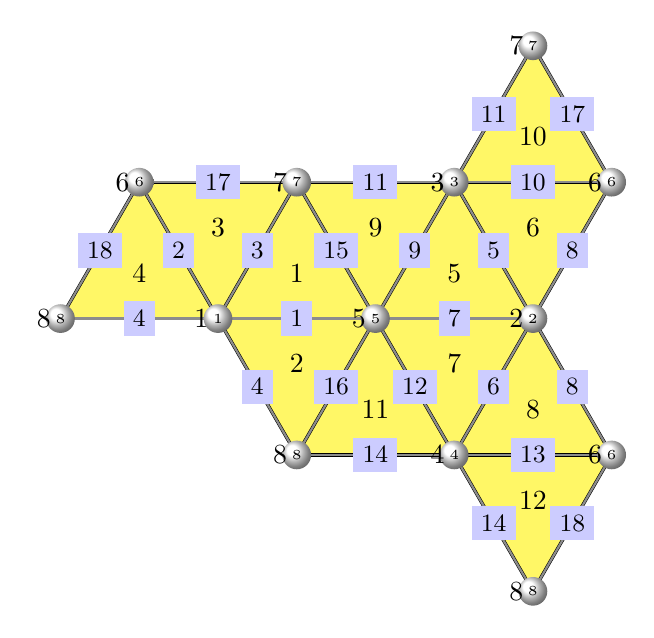
\begin{tikzpicture}[vertexBall, edgeDouble, faceStyle, scale=2]

% Define the coordinates of the vertices
\coordinate (V1_1) at (0., 0.);
\coordinate (V2_1) at (2., 0.);
\coordinate (V3_1) at (1.5, 0.8660254037844386);
\coordinate (V4_1) at (1.5, -0.8660254037844386);
\coordinate (V5_1) at (1., 0.);
\coordinate (V6_1) at (-0.4999999999999999, 0.8660254037844386);
\coordinate (V6_2) at (2.5, 0.8660254037844386);
\coordinate (V6_3) at (2.5, -0.8660254037844386);
\coordinate (V7_1) at (0.5, 0.8660254037844386);
\coordinate (V7_2) at (2., 1.732050807568877);
\coordinate (V8_1) at (0.5, -0.8660254037844386);
\coordinate (V8_2) at (-0.9999999999999998, 0.);
\coordinate (V8_3) at (2., -1.732050807568877);


% Fill in the faces
\fill[face]  (V5_1) -- (V7_1) -- (V1_1) -- cycle;
\node[faceLabel] at (barycentric cs:V5_1=1,V7_1=1,V1_1=1) {$1$};
\fill[face]  (V1_1) -- (V8_1) -- (V5_1) -- cycle;
\node[faceLabel] at (barycentric cs:V1_1=1,V8_1=1,V5_1=1) {$2$};
\fill[face]  (V7_1) -- (V6_1) -- (V1_1) -- cycle;
\node[faceLabel] at (barycentric cs:V7_1=1,V6_1=1,V1_1=1) {$3$};
\fill[face]  (V6_1) -- (V8_2) -- (V1_1) -- cycle;
\node[faceLabel] at (barycentric cs:V6_1=1,V8_2=1,V1_1=1) {$4$};
\fill[face]  (V5_1) -- (V2_1) -- (V3_1) -- cycle;
\node[faceLabel] at (barycentric cs:V5_1=1,V2_1=1,V3_1=1) {$5$};
\fill[face]  (V2_1) -- (V6_2) -- (V3_1) -- cycle;
\node[faceLabel] at (barycentric cs:V2_1=1,V6_2=1,V3_1=1) {$6$};
\fill[face]  (V5_1) -- (V4_1) -- (V2_1) -- cycle;
\node[faceLabel] at (barycentric cs:V5_1=1,V4_1=1,V2_1=1) {$7$};
\fill[face]  (V4_1) -- (V6_3) -- (V2_1) -- cycle;
\node[faceLabel] at (barycentric cs:V4_1=1,V6_3=1,V2_1=1) {$8$};
\fill[face]  (V5_1) -- (V3_1) -- (V7_1) -- cycle;
\node[faceLabel] at (barycentric cs:V5_1=1,V3_1=1,V7_1=1) {$9$};
\fill[face]  (V6_2) -- (V7_2) -- (V3_1) -- cycle;
\node[faceLabel] at (barycentric cs:V6_2=1,V7_2=1,V3_1=1) {$10$};
\fill[face]  (V5_1) -- (V8_1) -- (V4_1) -- cycle;
\node[faceLabel] at (barycentric cs:V5_1=1,V8_1=1,V4_1=1) {$11$};
\fill[face]  (V4_1) -- (V8_3) -- (V6_3) -- cycle;
\node[faceLabel] at (barycentric cs:V4_1=1,V8_3=1,V6_3=1) {$12$};


% Draw the edges
\draw[edge] (V5_1) -- node[edgeLabel] {$1$} (V1_1);
\draw[edge] (V1_1) -- node[edgeLabel] {$2$} (V6_1);
\draw[edge] (V1_1) -- node[edgeLabel] {$3$} (V7_1);
\draw[edge] (V8_1) -- node[edgeLabel] {$4$} (V1_1);
\draw[edge] (V1_1) -- node[edgeLabel] {$4$} (V8_2);
\draw[edge] (V3_1) -- node[edgeLabel] {$5$} (V2_1);
\draw[edge] (V2_1) -- node[edgeLabel] {$6$} (V4_1);
\draw[edge] (V2_1) -- node[edgeLabel] {$7$} (V5_1);
\draw[edge] (V6_2) -- node[edgeLabel] {$8$} (V2_1);
\draw[edge] (V2_1) -- node[edgeLabel] {$8$} (V6_3);
\draw[edge] (V3_1) -- node[edgeLabel] {$9$} (V5_1);
\draw[edge] (V3_1) -- node[edgeLabel] {$10$} (V6_2);
\draw[edge] (V7_1) -- node[edgeLabel] {$11$} (V3_1);
\draw[edge] (V3_1) -- node[edgeLabel] {$11$} (V7_2);
\draw[edge] (V4_1) -- node[edgeLabel] {$12$} (V5_1);
\draw[edge] (V6_3) -- node[edgeLabel] {$13$} (V4_1);
\draw[edge] (V4_1) -- node[edgeLabel] {$14$} (V8_1);
\draw[edge] (V8_3) -- node[edgeLabel] {$14$} (V4_1);
\draw[edge] (V7_1) -- node[edgeLabel] {$15$} (V5_1);
\draw[edge] (V5_1) -- node[edgeLabel] {$16$} (V8_1);
\draw[edge] (V6_1) -- node[edgeLabel] {$17$} (V7_1);
\draw[edge] (V7_2) -- node[edgeLabel] {$17$} (V6_2);
\draw[edge] (V8_2) -- node[edgeLabel] {$18$} (V6_1);
\draw[edge] (V6_3) -- node[edgeLabel] {$18$} (V8_3);


% Draw the vertices
\vertexLabelR{V1_1}{left}{$1$}
\vertexLabelR{V2_1}{left}{$2$}
\vertexLabelR{V3_1}{left}{$3$}
\vertexLabelR{V4_1}{left}{$4$}
\vertexLabelR{V5_1}{left}{$5$}
\vertexLabelR{V6_1}{left}{$6$}
\vertexLabelR{V6_2}{left}{$6$}
\vertexLabelR{V6_3}{left}{$6$}
\vertexLabelR{V7_1}{left}{$7$}
\vertexLabelR{V7_2}{left}{$7$}
\vertexLabelR{V8_1}{left}{$8$}
\vertexLabelR{V8_2}{left}{$8$}
\vertexLabelR{V8_3}{left}{$8$}

\end{tikzpicture}

\end{center}
 

 Construction of a butterfly 

 
\begin{Verbatim}[commandchars=!@|,fontsize=\small,frame=single,label=Example]
  !gapprompt@gap>| !gapinput@bufl:=function()|
  !gapprompt@>| !gapinput@return SimplicialSurfaceByVerticesInFaces([[1,2,3],[2,3,4]]);|
  !gapprompt@>| !gapinput@end;|
  function(  ) ... end
  !gapprompt@gap>| !gapinput@bufl();|
  simplicial surface ( 4 vertices, 5 edges, 2 faces)
\end{Verbatim}
 

 
\begin{center}
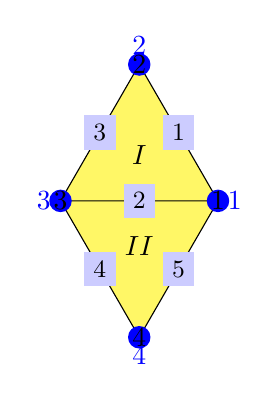
\begin{tikzpicture}[vertexStyle, edgeStyle, faceStyle]
    \def\hor{1}
    \def\ver{1.732}
    \coordinate (P1) at (0,0);
    \coordinate (P2) at (-\hor,\ver);
    \coordinate (P3) at (-2*\hor,0);
    \coordinate (P4) at (-\hor,-\ver);

	\ifdefined\join
		\draw[edge, face]
		        (P1) -- node[edgeLabel]{1} (P2) -- node[edgeLabel]{3} (P3) -- node[edgeLabel]{7} cycle
			(P4) -- node[edgeLabel]{4} (P3) -- node[edgeLabel]{7} (P1) -- node[edgeLabel]{5} cycle;
		\foreach \p/\r/\n in {P1/right/8, P2/above/3, P3/left/7, P4/below/6}{
		\vertexLabelR{\p}{\r}{\n}
		}
	\else
		\draw[edge, face]
		        (P1) -- node[edgeLabel]{1} (P2) -- node[edgeLabel]{3} (P3) -- node[edgeLabel]{3} cycle
			(P4) -- node[edgeLabel]{4} (P3) -- node[edgeLabel]{2} (P1) -- node[edgeLabel]{5} cycle;
		\foreach \p/\r/\n in {P1/right/1, P2/above/2, P3/left/3, P4/below/4}{
		\vertexLabelR{\p}{\r}{\n}
		}
	\fi
	\node[faceLabel] at (barycentric cs:P1=1,P2=1,P3=1) {$I$};
	\node[faceLabel] at (barycentric cs:P4=1,P3=1,P1=1) {$II$};
\end{tikzpicture}

\end{center}
 Define the function \texttt{checkbufl()} which checks whether a given edge is an inner edge giving rise to a butterfly
in the surface. 

 
\begin{Verbatim}[commandchars=!@|,fontsize=\small,frame=single,label=Example]
  !gapprompt@gap>| !gapinput@checkbufl:=function(S,e)|
  !gapprompt@>| !gapinput@local sS;|
  !gapprompt@>| !gapinput@if not (e in InnerEdges(S)) then Error("not inner");fi;|
  !gapprompt@>| !gapinput@sS:=FacesOfEdge(S,e);|
  !gapprompt@>| !gapinput@sS:=SubcomplexByFaces(S,sS);|
  !gapprompt@>| !gapinput@return IsIsomorphic(bufl(),sS);|
  !gapprompt@>| !gapinput@end;|
  function( S, e ) ... end
  
  !gapprompt@gap>| !gapinput@checkbufl(PE,2);|
  true
\end{Verbatim}
 

 If the function returns true, the butterfly of the edge e can be turned. Here
the program to perform an edgeturn is introduced: 
\begin{Verbatim}[commandchars=!@|,fontsize=\small,frame=single,label=Example]
  !gapprompt@gap>| !gapinput@turnedge:=function(S,e)|
  !gapprompt@>| !gapinput@local sS,sB,v,ee;|
  !gapprompt@>| !gapinput@sB:=SubcomplexByFaces(S,FacesOfEdge(S,e));|
  !gapprompt@>| !gapinput@ee:=Difference(Edges(sB),[e]);|
  !gapprompt@>| !gapinput@v:=Intersection(VerticesOfEdge(sB,ee[1]),VerticesOfEdge(S,e))[1];|
  !gapprompt@>| !gapinput@sS:=Difference(Faces(S),FacesOfEdge(S,e));|
  !gapprompt@>| !gapinput@sS:=SubcomplexByFaces(S,sS);|
  !gapprompt@>| !gapinput@return JoinBoundaries(sS,[v,ee[1]],sB,|
  !gapprompt@>| !gapinput@[Difference(VerticesOfEdge(sB,ee[1]),[v])[1],ee[1]]);|
  !gapprompt@>| !gapinput@end;|
  function( S, e ) ... end
\end{Verbatim}
 

 The vertex-counter of the simplicial parallelepiped is [[3,2],[5,6]]. So turn
an edge incident to vertex 1 to create a vertex of degree 3 and vertices of
degree 5. 
\begin{Verbatim}[commandchars=!@|,fontsize=\small,frame=single,label=Example]
  !gapprompt@gap>| !gapinput@VerticesOfEdges(PE);|
  [ [ 1, 2 ], [ 1, 3 ], [ 1, 4 ], [ 1, 5 ], [ 1, 6 ], [ 1, 7 ], [ 2, 3 ], [ 2, 7 ], 
   [ 2, 8 ], [ 3, 4 ], [ 3, 8 ], [ 4, 5 ], [ 4, 8 ], [ 5, 6 ], [ 5, 8 ], [ 6, 7 ], 
   [ 6, 8 ], [ 7, 8 ] ]
  !gapprompt@gap>| !gapinput@turnedge(PE,1);|
  [ simplicial surface (8 vertices, 18 edges, and 12 faces)
     , ( v26, E27, v27, E28, v28, E29, v29, E30, v26 )
     , 18 ]
  !gapprompt@gap>| !gapinput@PE1:=last[1];|
  simplicial surface (8 vertices, 18 edges, and 12 faces)
\end{Verbatim}
 

 Compute the face degrees of the vertices 
\begin{Verbatim}[commandchars=!@|,fontsize=\small,frame=single,label=Example]
  !gapprompt@gap>| !gapinput@FaceDegreesOfVertices(PE1);|
  [ ,,, 4, 4, 4,, 6,,,,,,,,,,,,,,,,,, 5, 5, 3, 5 ]
\end{Verbatim}
 

 Since the face degrees of the vertices 4,5,6 and 8 is neither 3 or 5, we need
to find an inner edge so that the resulting butterfly contains the vertices
[4,5,6,8]. 

 
\begin{Verbatim}[commandchars=!@|,fontsize=\small,frame=single,label=Example]
  !gapprompt@gap>| !gapinput@Filtered(Faces(PE1),f->IsSubset([4,5,6,8],VerticesOfFace(PE1,f)));|
  [ 8, 10 ]
  !gapprompt@gap>| !gapinput@Intersection(EdgesOfFace(PE1,8),EdgesOfFace(PE1,10));|
  [ 15 ]
\end{Verbatim}
 

 From this information we can compute the simplicial parallelepiped by turning
edge 15 

 
\begin{Verbatim}[commandchars=!@|,fontsize=\small,frame=single,label=Example]
  !gapprompt@gap>| !gapinput@turnedge(PE1,15);|
  [ simplicial surface (8 vertices, 18 edges, and 12 faces)
     , ( v39, E48, v40, E49, v41, E50, v42, E51, v39 )
     , 30 ]
  !gapprompt@gap>| !gapinput@PE3:=last[1];|
  simplicial surface (8 vertices, 18 edges, and 12 faces)
\end{Verbatim}
 

 By calling the vertex counter we see that the sphere is indeed isomorphic to
the simplicial parallelepiped. 

 
\begin{Verbatim}[commandchars=!@|,fontsize=\small,frame=single,label=Example]
  !gapprompt@gap>| !gapinput@VertexCounter(PE3);|
  [ [ 3, 2 ], [ 5, 6 ] ]
\end{Verbatim}
 }

 
\subsection{\textcolor{Chapter }{Construction using the barycentric subdivision and edge-turns}}\label{Chapter_Tutorial_Section_Parallelelepiped_Subsection_Construction_using_the_barycentric_subdivision_and_edge-turns}
\logpage{[ 3, 1, 5 ]}
\hyperdef{L}{X7B89B4117D6E1CAD}{}
{
  

 $Idea$ $behind$ $the$ $construcion$ 

 The Janus Head is a closed simplicial surface with 2 faces whose barycentric
subdivision is a sphere with 12 faces. From this information we can deduce
that performing edgeturns on the resulting surface gives rise to a simplicial
parallelepiped. 

 
\begin{center}


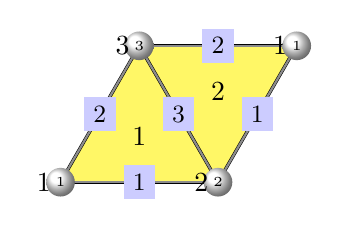
\begin{tikzpicture}[vertexBall, edgeDouble, faceStyle, scale=2]

% Define the coordinates of the vertices
\coordinate (V1_1) at (0, 0);
\coordinate (V2_1) at (1, 0);
\coordinate (V3_1) at (0.5, 0.8660254037844386);
\coordinate (V4_1) at (1.5, 0.8660254037844386);


% Fill in the faces
\fill[face]  (V2_1) -- (V3_1) -- (V1_1) -- cycle;
\node[faceLabel] at (barycentric cs:V2_1=1,V3_1=1,V1_1=1) {$1$};
\fill[face]  (V2_1) -- (V4_1) -- (V3_1) -- cycle;
\node[faceLabel] at (barycentric cs:V2_1=1,V4_1=1,V3_1=1) {$2$};


% Draw the edges
\draw[edge] (V2_1) -- node[edgeLabel] {$1$} (V1_1);
\draw[edge] (V1_1) -- node[edgeLabel] {$2$} (V3_1);
\draw[edge] (V3_1) -- node[edgeLabel] {$3$} (V2_1);
\draw[edge] (V4_1) -- node[edgeLabel] {$1$} (V2_1);
\draw[edge] (V3_1) -- node[edgeLabel] {$2$} (V4_1);


% Draw the vertices
\vertexLabelR{V1_1}{left}{$1$}
\vertexLabelR{V2_1}{left}{$2$}
\vertexLabelR{V3_1}{left}{$3$}
\vertexLabelR{V4_1}{left}{$1$}

\end{tikzpicture}

\end{center}
 

 Compute the Janus Head 

 
\begin{Verbatim}[commandchars=!@|,fontsize=\small,frame=single,label=Example]
  !gapprompt@gap>| !gapinput@J:=JanusHead();|
  simplicial surface ( 3 vertices, 3 edges, 2 faces)
  !gapprompt@gap>| !gapinput@Checkbufl(J,1);|
  false
\end{Verbatim}
 

 Constructing the Janus-Head's barycentric subdivision 

 
\begin{Verbatim}[commandchars=!@|,fontsize=\small,frame=single,label=Example]
  !gapprompt@gap>| !gapinput@BJ:=FlagSurface(J);|
  coloured surface (MMM with 8 vertices, 18 edges and 12 faces)
  !gapprompt@gap>| !gapinput@FaceDegreesOfVertices(BJ);|
  [ 4, 4, 4, 4, 4, 4, 6, 6 ]
\end{Verbatim}
 

 
\begin{center}


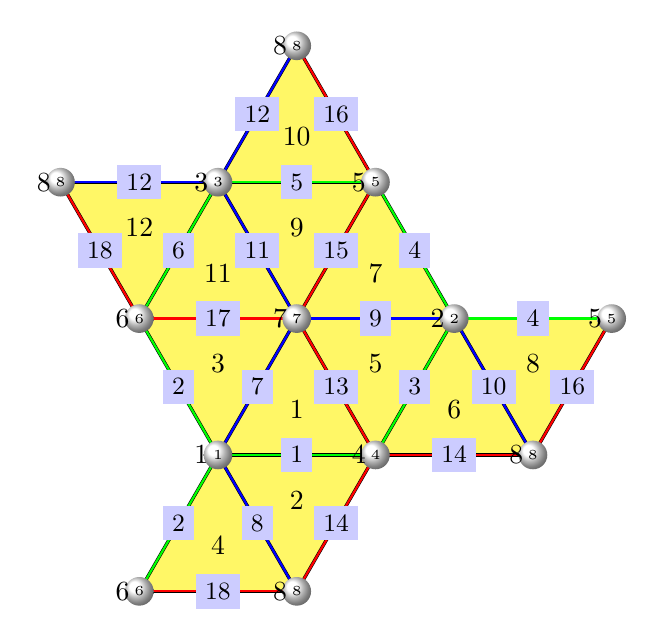
\begin{tikzpicture}[vertexBall, edgeDouble, faceStyle, scale=2]

% Define the coordinates of the vertices
\coordinate (V1_1) at (0, 0);
\coordinate (V2_1) at (1.5, 0.8660254037844387);
\coordinate (V3_1) at (0, 1.732050807568877);
\coordinate (V4_1) at (1, 0);
\coordinate (V5_1) at (0.9999999999999997, 1.732050807568877);
\coordinate (V5_2) at (2.5, 0.8660254037844389);
\coordinate (V6_1) at (-0.5, 0.8660254037844384);
\coordinate (V6_2) at (-0.4999999999999998, -0.8660254037844388);
\coordinate (V7_1) at (0.4999999999999999, 0.8660254037844386);
\coordinate (V8_1) at (0.5000000000000001, -0.8660254037844386);
\coordinate (V8_2) at (2, 0);
\coordinate (V8_3) at (0.4999999999999997, 2.598076211353315);
\coordinate (V8_4) at (-0.9999999999999999, 1.732050807568877);


% Fill in the faces
\fill[face]  (V4_1) -- (V7_1) -- (V1_1) -- cycle;
\node[faceLabel] at (barycentric cs:V4_1=1,V7_1=1,V1_1=1) {$1$};
\fill[face]  (V1_1) -- (V8_1) -- (V4_1) -- cycle;
\node[faceLabel] at (barycentric cs:V1_1=1,V8_1=1,V4_1=1) {$2$};
\fill[face]  (V7_1) -- (V6_1) -- (V1_1) -- cycle;
\node[faceLabel] at (barycentric cs:V7_1=1,V6_1=1,V1_1=1) {$3$};
\fill[face]  (V1_1) -- (V6_2) -- (V8_1) -- cycle;
\node[faceLabel] at (barycentric cs:V1_1=1,V6_2=1,V8_1=1) {$4$};
\fill[face]  (V4_1) -- (V2_1) -- (V7_1) -- cycle;
\node[faceLabel] at (barycentric cs:V4_1=1,V2_1=1,V7_1=1) {$5$};
\fill[face]  (V4_1) -- (V8_2) -- (V2_1) -- cycle;
\node[faceLabel] at (barycentric cs:V4_1=1,V8_2=1,V2_1=1) {$6$};
\fill[face]  (V2_1) -- (V5_1) -- (V7_1) -- cycle;
\node[faceLabel] at (barycentric cs:V2_1=1,V5_1=1,V7_1=1) {$7$};
\fill[face]  (V8_2) -- (V5_2) -- (V2_1) -- cycle;
\node[faceLabel] at (barycentric cs:V8_2=1,V5_2=1,V2_1=1) {$8$};
\fill[face]  (V5_1) -- (V3_1) -- (V7_1) -- cycle;
\node[faceLabel] at (barycentric cs:V5_1=1,V3_1=1,V7_1=1) {$9$};
\fill[face]  (V5_1) -- (V8_3) -- (V3_1) -- cycle;
\node[faceLabel] at (barycentric cs:V5_1=1,V8_3=1,V3_1=1) {$10$};
\fill[face]  (V3_1) -- (V6_1) -- (V7_1) -- cycle;
\node[faceLabel] at (barycentric cs:V3_1=1,V6_1=1,V7_1=1) {$11$};
\fill[face]  (V3_1) -- (V8_4) -- (V6_1) -- cycle;
\node[faceLabel] at (barycentric cs:V3_1=1,V8_4=1,V6_1=1) {$12$};


% Draw the edges
\draw[edge=green] (V4_1) -- node[edgeLabel] {$1$} (V1_1);
\draw[edge=green] (V1_1) -- node[edgeLabel] {$2$} (V6_1);
\draw[edge=green] (V6_2) -- node[edgeLabel] {$2$} (V1_1);
\draw[edge=green] (V2_1) -- node[edgeLabel] {$3$} (V4_1);
\draw[edge=green] (V5_1) -- node[edgeLabel] {$4$} (V2_1);
\draw[edge=green] (V2_1) -- node[edgeLabel] {$4$} (V5_2);
\draw[edge=green] (V3_1) -- node[edgeLabel] {$5$} (V5_1);
\draw[edge=green] (V6_1) -- node[edgeLabel] {$6$} (V3_1);
\draw[edge=blue] (V1_1) -- node[edgeLabel] {$7$} (V7_1);
\draw[edge=blue] (V8_1) -- node[edgeLabel] {$8$} (V1_1);
\draw[edge=blue] (V7_1) -- node[edgeLabel] {$9$} (V2_1);
\draw[edge=blue] (V2_1) -- node[edgeLabel] {$10$} (V8_2);
\draw[edge=blue] (V7_1) -- node[edgeLabel] {$11$} (V3_1);
\draw[edge=blue] (V3_1) -- node[edgeLabel] {$12$} (V8_3);
\draw[edge=blue] (V8_4) -- node[edgeLabel] {$12$} (V3_1);
\draw[edge=red] (V7_1) -- node[edgeLabel] {$13$} (V4_1);
\draw[edge=red] (V4_1) -- node[edgeLabel] {$14$} (V8_1);
\draw[edge=red] (V8_2) -- node[edgeLabel] {$14$} (V4_1);
\draw[edge=red] (V7_1) -- node[edgeLabel] {$15$} (V5_1);
\draw[edge=red] (V5_2) -- node[edgeLabel] {$16$} (V8_2);
\draw[edge=red] (V8_3) -- node[edgeLabel] {$16$} (V5_1);
\draw[edge=red] (V6_1) -- node[edgeLabel] {$17$} (V7_1);
\draw[edge=red] (V8_1) -- node[edgeLabel] {$18$} (V6_2);
\draw[edge=red] (V6_1) -- node[edgeLabel] {$18$} (V8_4);


% Draw the vertices
\vertexLabelR{V1_1}{left}{$1$}
\vertexLabelR{V2_1}{left}{$2$}
\vertexLabelR{V3_1}{left}{$3$}
\vertexLabelR{V4_1}{left}{$4$}
\vertexLabelR{V5_1}{left}{$5$}
\vertexLabelR{V5_2}{left}{$5$}
\vertexLabelR{V6_1}{left}{$6$}
\vertexLabelR{V6_2}{left}{$6$}
\vertexLabelR{V7_1}{left}{$7$}
\vertexLabelR{V8_1}{left}{$8$}
\vertexLabelR{V8_2}{left}{$8$}
\vertexLabelR{V8_3}{left}{$8$}
\vertexLabelR{V8_4}{left}{$8$}

\end{tikzpicture}
\end{center}
 

 Which edges have to be turned to obtain the parallelepiped? The vertex counter
of the surface \texttt{BJ} is \texttt{[[4,6],[6,4]]}. To create a sphere with the vertex counter \texttt{[[3,2],[5,6]]}, we first have to find an edge incident to vertices with degree 6 and 4.
Their degree will decrease by 1 and the vertex degrees of the vertices
incident to the orthogonal edge will increase by 1. 

 
\begin{Verbatim}[commandchars=!@|,fontsize=\small,frame=single,label=Example]
  VerticesOfEdges(BJ);
  [ [ 1, 4 ], [ 1, 5 ], [ 2, 4 ], [ 2, 6 ], [ 3, 5 ], [ 3, 6 ], [ 1, 7 ], 
   [ 1, 8 ], [ 2, 7 ], [ 2, 8 ], [ 3, 7 ], [ 3, 8 ], [ 4, 7 ], [ 4, 8 ], 
   [ 5, 7 ], [ 5, 8 ], [ 6, 7 ], [ 6, 8 ] ]
  !gapprompt@gap>| !gapinput@BJ1:=turnedge(BJ,18)[1];|
  simplicial surface (8 vertices, 18 edges, 12 faces)
\end{Verbatim}
 

 Computing face degrees of the vertices 

 
\begin{Verbatim}[commandchars=!@|,fontsize=\small,frame=single,label=Example]
  !gapprompt@gap>| !gapinput@FaceDegreesOfVertices(BJ1);|
  [ 4,,, 4, 4,, 6,,,,,,,,,,,,,,,,,,, 3, 5, 5, 5 ]
\end{Verbatim}
 

 Find an edge incident to a vertex with face degree 4 and another vertex with
degree 6. For that we may use 

 
\begin{Verbatim}[commandchars=!@|,fontsize=\small,frame=single,label=Example]
  !gapprompt@gap>| !gapinput@VerticesOfEdges(BJ1);|
  [ [ 1, 4 ], [ 1, 5 ], [ 4, 27 ],, [ 5, 29 ],, [ 1, 7 ], [ 1, 28 ], [ 7, 27 ],
   , [ 7, 29 ],, [ 4, 7 ], [ 4, 28 ], [ 5, 7 ], [ 5, 28 ], [ 7, 26 ],,,,,,,,,,
   ,,,,,,,, [ 27, 29 ], [ 26, 27 ], [ 27, 28 ], [ 28, 29 ], [ 26, 29 ] ]
  !gapprompt@gap>| !gapinput@Position(last,[1,7]);|
  7
  !gapprompt@gap>| !gapinput@JB2:=turnedge(BJ1,7)[1];|
  simplicial surface (8 vertices, 18 edges, 12 faces)
  !gapprompt@gap>| !gapinput@FaceDegreesOfVertices(JB2);|
  [ ,,,,,,,,,,,,,,,,,,,,,,,,, 3, 5, 5, 5,,,,,,,,,,,,,,,,,, 3, 5, 5, 5 ]
\end{Verbatim}
 

 Check whether the constructed surface is isomorphic to the simplicial
parallelepiped 

 
\begin{Verbatim}[commandchars=!@|,fontsize=\small,frame=single,label=Example]
  !gapprompt@gap>| !gapinput@IsIsomorphic(JB2,PEs);|
  true
\end{Verbatim}
 

 The surface is vertex-faithful. Hence we easily can clean up the sets of
vertices, edges and faces 

 
\begin{Verbatim}[commandchars=!@|,fontsize=\small,frame=single,label=Example]
  !gapprompt@gap>| !gapinput@V:=Vertices(JB2);|
  [ 26, 27, 28, 29, 47, 48, 49, 50 ]
  !gapprompt@gap>| !gapinput@FF:=VerticesOfFaces(JB2);|
  [ , [ 28, 47, 48 ],, [ 28, 47, 50 ], [ 27, 48, 49 ], [ 27, 28, 48 ], 
   [ 26, 27, 49 ],, [ 29, 49, 50 ], [ 28, 29, 50 ], [ 26, 29, 49 ],,,,,,,,,,,,
   ,, [ 26, 27, 29 ],,,, [ 27, 28, 29 ],,,,,,,,,,, [ 47, 48, 50 ],, 
   [ 48, 49, 50 ] ]
  !gapprompt@gap>| !gapinput@FF:=Set(FF);|
  [ [ 26, 27, 29 ], [ 26, 27, 49 ], [ 26, 29, 49 ], [ 27, 28, 29 ], 
   [ 27, 28, 48 ], [ 27, 48, 49 ], [ 28, 29, 50 ], [ 28, 47, 48 ], 
   [ 28, 47, 50 ], [ 29, 49, 50 ], [ 47, 48, 50 ], [ 48, 49, 50 ] ]
  !gapprompt@gap>| !gapinput@FF:=List(FF,r->List(r,i->Position(V,i)));|
  [ [ 1, 2, 4 ], [ 1, 2, 7 ], [ 1, 4, 7 ], [ 2, 3, 4 ], [ 2, 3, 6 ], 
   [ 2, 6, 7 ], [ 3, 4, 8 ], [ 3, 5, 6 ], [ 3, 5, 8 ], [ 4, 7, 8 ], 
   [ 5, 6, 8 ], [ 6, 7, 8 ] ]
  !gapprompt@gap>| !gapinput@PEt:=SimplicialSurfaceByVerticesInFaces(FF);|
  simplicial surface (8 vertices, 18 edges, and 12 faces)
  !gapprompt@gap>| !gapinput@FaceDegreesOfVertices(PEt);|
  [ 3, 5, 5, 5, 3, 5, 5, 5 ]
  !gapprompt@gap>| !gapinput@Vertices(PEt);|
  [ 1, 2, 3, 4, 5, 6, 7, 8 ]
\end{Verbatim}
 

 We want to understand the barycentric subdivision of the Janus head better.
Indeed we shall see that it is isomorphic to the double 6-gon. 

 Define a function that creates a n-gon 

 
\begin{Verbatim}[commandchars=!@|,fontsize=\small,frame=single,label=Example]
  !gapprompt@gap>| !gapinput@ngon:=function(n)|
  !gapprompt@>| !gapinput@local c,L;|
  !gapprompt@>| !gapinput@c:=CycleFromList([1..n]);|
  !gapprompt@>| !gapinput@L:=List([1..n],i->[i,i^c,n+1]);|
  !gapprompt@>| !gapinput@return SimplicialSurfaceByVerticesInFaces(L);|
  !gapprompt@>| !gapinput@end;|
  function( n ) ... end
\end{Verbatim}
 

 Compute the 4-gon 

 
\begin{Verbatim}[commandchars=!@|,fontsize=\small,frame=single,label=Example]
  !gapprompt@gap>| !gapinput@ngon(4);|
  simplicial surface (5 vertices, 8 edges, and 4 faces)
\end{Verbatim}
 

 
\begin{center}


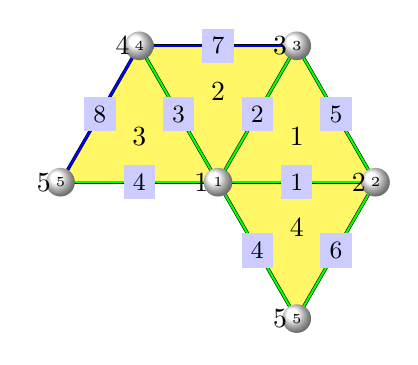
\begin{tikzpicture}[vertexBall, edgeDouble, faceStyle, scale=2]

% Define the coordinates of the vertices
\coordinate (V1_1) at (0, 0);
\coordinate (V2_1) at (1, 0);
\coordinate (V3_1) at (0.5, 0.8660254037844386);
\coordinate (V4_1) at (-0.4999999999999999, 0.8660254037844386);
\coordinate (V5_1) at (0.5, -0.8660254037844386);
\coordinate (V5_2) at (-0.9999999999999998, 0);


% Fill in the faces
\fill[face]  (V2_1) -- (V3_1) -- (V1_1) -- cycle;
\node[faceLabel] at (barycentric cs:V2_1=1,V3_1=1,V1_1=1) {$1$};
\fill[face]  (V3_1) -- (V4_1) -- (V1_1) -- cycle;
\node[faceLabel] at (barycentric cs:V3_1=1,V4_1=1,V1_1=1) {$2$};
\fill[face]  (V4_1) -- (V5_2) -- (V1_1) -- cycle;
\node[faceLabel] at (barycentric cs:V4_1=1,V5_2=1,V1_1=1) {$3$};
\fill[face]  (V1_1) -- (V5_1) -- (V2_1) -- cycle;
\node[faceLabel] at (barycentric cs:V1_1=1,V5_1=1,V2_1=1) {$4$};


% Draw the edges
\draw[edge=green] (V2_1) -- node[edgeLabel] {$1$} (V1_1);
\draw[edge=green] (V1_1) -- node[edgeLabel] {$2$} (V3_1);
\draw[edge=green] (V1_1) -- node[edgeLabel] {$3$} (V4_1);
\draw[edge=green] (V5_1) -- node[edgeLabel] {$4$} (V1_1);
\draw[edge=green] (V1_1) -- node[edgeLabel] {$4$} (V5_2);
\draw[edge=green] (V3_1) -- node[edgeLabel] {$5$} (V2_1);
\draw[edge=green] (V2_1) -- node[edgeLabel] {$6$} (V5_1);
\draw[edge=blue] (V4_1) -- node[edgeLabel] {$7$} (V3_1);
\draw[edge=blue] (V5_2) -- node[edgeLabel] {$8$} (V4_1);


% Draw the vertices
\vertexLabelR{V1_1}{left}{$1$}
\vertexLabelR{V2_1}{left}{$2$}
\vertexLabelR{V3_1}{left}{$3$}
\vertexLabelR{V4_1}{left}{$4$}
\vertexLabelR{V5_1}{left}{$5$}
\vertexLabelR{V5_2}{left}{$5$}

\end{tikzpicture}
\end{center}
 

 Define a function to create a double-n-gon 

 
\begin{Verbatim}[commandchars=!@|,fontsize=\small,frame=single,label=Example]
  !gapprompt@gap>| !gapinput@Doublengon:=function(n)|
  !gapprompt@>| !gapinput@local c,L1,L2;|
  !gapprompt@>| !gapinput@c:=CycleFromList([1..n]);|
  !gapprompt@>| !gapinput@L1:=List([1..n],i->[i,i^c,n+1]);|
  !gapprompt@>| !gapinput@L2:=List([1..n],i->[i,i^c,n+2]);|
  !gapprompt@>| !gapinput@L1:=Union(L1,L2);|
  !gapprompt@>| !gapinput@return SimplicialSurfaceByVerticesInFaces(L1);|
  !gapprompt@>| !gapinput@end;|
  function( n ) ... end
\end{Verbatim}
 

 Verify that the barycentric subdivision of the Janus Head is isomorphic to the
double-6-gon 

 
\begin{Verbatim}[commandchars=!@|,fontsize=\small,frame=single,label=Example]
  !gapprompt@gap>| !gapinput@Doublengon(4);|
  simplicial surface (6 vertices, 12 edges, and 8 faces)
  !gapprompt@gap>| !gapinput@IsIsomorphic(Doublengon(4),Octahedron());|
  true
  !gapprompt@gap>| !gapinput@IsIsomorphic(Doublengon(6),BJ);|
  true
  !gapprompt@gap>| !gapinput@FaceDegreesOfVertices(Doublengon(7));|
  [ 4, 4, 4, 4, 4, 4, 4, 7, 7 ]
\end{Verbatim}
 }

 
\subsection{\textcolor{Chapter }{Construction using power sets}}\label{Chapter_Tutorial_Section_Parallelelepiped_Subsection_Construction_using_power_sets}
\logpage{[ 3, 1, 6 ]}
\hyperdef{L}{X840F7C2C82556810}{}
{
  

 $Idea$ $behind$ $the$ $construcion$ 

 The construction of the simplicial parallelepiped can be achieved by using the
power set of \texttt{[1,2,3].} The power set forms the set of vertices of the parallelepiped. So we refer to
the different subsets of [1,2,3] as vertices. Since the surface is
vertex-faithful, we see that constructing the surface can be achieved by
determining the vertices of faces. The set of vertices of a face can be
written as [V1,V2,V3] where the subsets V1 and V2 have the same cardinalty and
V3 is either the intersection or the union of V1 and V2. 

 
\begin{center}
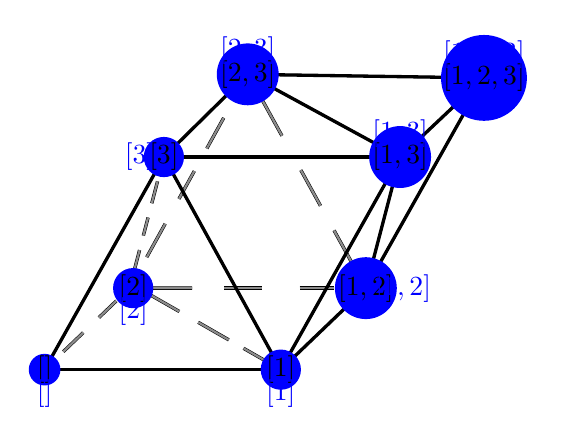
\begin{tikzpicture}[vertexStyle, edgeDouble, faceStyle, scale=0.75]

\coordinate (A) at (2,0);
\coordinate (B) at (-2,0);
\coordinate (C) at (4.02,3.6);
\coordinate (D) at (1.44,5);
\coordinate (E) at (3.44,1.38);
\coordinate (F) at (5.44,4.94);
\coordinate (G) at (0.02,3.6);
\coordinate (H) at (-0.5,1.38);
\coordinate (E1) at (3.44,1.5);

%\coordinate (V5_1) at (-2.927759705906105,0.2473194530248809);
%\coordinate (V6_1) at (-0.01834378355858286,-2.8699118923474716);
%\coordinate (V1_1) at (-0.07029763931478862,2.758422481241498);
%\coordinate (V2_1) at (0.6051024855158862,1.2344427123927926);

    

\draw [edge=black] (-2,0)-- (2,0);
\draw [edge=black] (4.02,3.6)-- (0.02,3.6);
\draw [edge=black] (0.02,3.6)-- (-2,0);
\draw [edge=black] (3.44,1.38)-- (5.44,4.94);
\draw [edge=black] (5.44,4.94)-- (1.44,5);
\draw [edge=black] (2,0)-- (3.44,1.38);
\draw [edge=black] (1.44,5)-- (0.02,3.6);
\draw [edge=black] (4.02,3.6)-- (5.44,4.94);
\draw [edge] (1.0332274736325155,4.263741727274853)-- (0.7467514791515633,3.7452201772643297);
\draw [edge] (0.5353438881223546,3.362572437501462)-- (0.27515352774724633,2.891627885222516);
\draw [edge] (0.04213746170575994,2.4698688056874256)-- (-0.2706241668810365,1.903770257945324);
\draw [edge] (-0.17237103195467773,1.380053770842896)-- (0.5,1.38);
\draw [edge] (1.04,1.38)-- (1.68,1.38);
\draw [edge] (2.32,1.38)-- (2.9,1.38);
\draw [edge] (-0.7850135746606335,1.1643619909502263)-- (-1.0803981900452488,0.8812850678733032);
\draw [edge] (-1.3462443438914027,0.6265158371040724)-- (-1.68289592760181,0.303891402714932);
\draw [edge=black] (1.445708891887561,5.001217790538086)-- (4.02,3.6);
\draw [edge=black] (4.02,3.6)-- (3.44,1.38);
\draw [edge] (-0.20657687221433152,1.2634432090904641)-- (0.28208649654699514,0.9836440221384141);
\draw [edge] (0.6006954988489983,0.801214674046138)-- (1.1194827839545476,0.5041671156389285);
\draw [edge] (1.3693663636853701,0.3610886143414413)-- (1.7904098214480486,0.12000727965474631);
\draw [edge] (1.6586800662532202,4.614506441153063)-- (2.0193178570905728,3.9596632345578975);
\draw [edge] (2.3391022653831035,3.3790012721517955)-- (2.672007457959911,2.7745146949325603);
\draw [edge] (2.901332820391631,2.35810754209451)-- (3.209287291452826,1.7989262847814618);
\draw [edge] (-0.08740460161040448,3.1888996283187967)-- (-0.18448630955407658,2.817311022051638);
\draw [edge] (-0.24757816479935152,2.57582150714731)-- (-0.327664946393825,2.2692824465615664);
\draw [edge] (-0.47394672494161083,1.7093763286717656)-- (-0.39168935199695565,2.024223514770273);
\draw [edge] (-0.56,1.38)-- (-0.4,1.38);
\draw [edge] (-0.56,1.38)-- (-0.6456793566202854,1.2978906165722264);
\draw [edge] (-0.56,1.38)-- (-0.5195862057533234,1.5160463805806987);
\draw [edge=black] (2,0)-- (0.02,3.6);
\draw [edge=black] (2,0)-- (4.02,3.6);

\foreach \p/\r/\n in {A/below/${[1]}$, B/below/${[]}$, C/above/${[1,3]}$, D/above/${[2,3]}$, E/right/${[1,2]}$}{
        \vertexLabelR{\p}{\r}{\n}
}
\foreach \p/\r/\n in {F/above/${[1,2,3]}$, G/left/${[3]}$, H/below/${[2]}$}{
        \vertexLabelR{\p}{\r}{\n}
}
\end{tikzpicture}


\end{center}
 

 Compute the ordered power set such that we can easily access subsets of a
given size. 
\begin{Verbatim}[commandchars=!@|,fontsize=\small,frame=single,label=Example]
  !gapprompt@gap>| !gapinput@powset:=List([0..3],i->Combinations([1,2,3],i));|
  [ [ [  ] ], [ [ 1 ], [ 2 ], [ 3 ] ], [ [ 1, 2 ], [ 1, 3 ], [ 2, 3 ] ], 
   [ [ 1, 2, 3 ] ] ]
\end{Verbatim}
 

 To compute the faces incident to exactly two vertices of cardinality 1, we
have to tell GAP to compute the union and intersection of those sets 

 
\begin{Verbatim}[commandchars=!@|,fontsize=\small,frame=single,label=Example]
  !gapprompt@gap>| !gapinput@t1:=List(Combinations(C[2],2),r->Union(r, [Intersection(r)]));|
  [ [ [  ], [ 1 ], [ 2 ] ], [ [  ], [ 1 ], [ 3 ] ], [ [  ], [ 2 ], [ 3 ] ] ]
  !gapprompt@gap>| !gapinput@t2:=List(Combinations(C[2],2),r->Union(r, [Union(r)]));|
  [ [ [ 1 ], [ 1, 2 ], [ 2 ] ], [ [ 1 ], [ 1, 3 ], [ 3 ] ], 
   [ [ 2 ], [ 2, 3 ], [ 3 ] ] ]
\end{Verbatim}
 

 Conpute the faces incident to exactly two vertices of cardinality 2 

 
\begin{Verbatim}[commandchars=!@|,fontsize=\small,frame=single,label=Example]
  !gapprompt@gap>| !gapinput@t3:=List(Combinations(C[3],2),r->Union(r, [Intersection(r)]));|
  [ [ [ 1 ], [ 1, 2 ], [ 1, 3 ] ], [ [ 1, 2 ], [ 2 ], [ 2, 3 ] ], 
   [ [ 1, 3 ], [ 2, 3 ], [ 3 ] ] ]
  !gapprompt@gap>| !gapinput@t4:=List(Combinations(C[3],2),r->Union(r, [Union(r)]));|
  [ [ [ 1, 2 ], [ 1 .. 3 ], [ 1, 3 ] ], [ [ 1, 2 ], [ 1 .. 3 ], [ 2, 3 ] ], 
   [ [ 1 .. 3 ], [ 1, 3 ], [ 2, 3 ] ] ]
\end{Verbatim}
 

 Compute the set of faces represented by their set of vertices 

 
\begin{Verbatim}[commandchars=!@|,fontsize=\small,frame=single,label=Example]
  !gapprompt@gap>| !gapinput@t:=Union([t1,t2,t3,t4]);|
  [ [ [  ], [ 1 ], [ 2 ] ], [ [  ], [ 1 ], [ 3 ] ], [ [  ], [ 2 ], [ 3 ] ], 
   [ [ 1 ], [ 1, 2 ], [ 1, 3 ] ], [ [ 1 ], [ 1, 2 ], [ 2 ] ], 
   [ [ 1 ], [ 1, 3 ], [ 3 ] ], [ [ 1, 2 ], [ 1 .. 3 ], [ 1, 3 ] ], 
   [ [ 1, 2 ], [ 1 .. 3 ], [ 2, 3 ] ], [ [ 1, 2 ], [ 2 ], [ 2, 3 ] ], 
   [ [ 1 .. 3 ], [ 1, 3 ], [ 2, 3 ] ], [ [ 1, 3 ], [ 2, 3 ], [ 3 ] ], 
   [ [ 2 ], [ 2, 3 ], [ 3 ] ] ]
\end{Verbatim}
 

 From this information we can already reclaim the simplicial parallelepiped,
but we notice that the vertices' labelling can be improved by calling 

 
\begin{Verbatim}[commandchars=!@|,fontsize=\small,frame=single,label=Example]
  !gapprompt@gap>| !gapinput@powset:=C[1];|
  [ [  ] ]
  !gapprompt@gap>| !gapinput@Append(powset,C[2]);|
  !gapprompt@gap>| !gapinput@Append(powset,C[3]);|
  !gapprompt@gap>| !gapinput@Append(powset,C[4]);|
  !gapprompt@gap>| !gapinput@powset; #powset is the power set|
  [ [  ], [ 1 ], [ 2 ], [ 3 ], [ 1, 2 ], [ 1, 3 ], [ 2, 3 ], [ 1, 2, 3 ] ]
  !gapprompt@gap>| !gapinput@verticesinfaces:=List(t,r->List(r,i->Position(powset,i)));|
  [ [ 1, 2, 3 ], [ 1, 2, 4 ], [ 1, 3, 4 ], [ 2, 5, 6 ], [ 2, 5, 3 ], 
   [ 2, 6, 4 ], [ 5, 8, 6 ], [ 5, 8, 7 ], [ 5, 3, 7 ], [ 8, 6, 7 ], 
   [ 6, 7, 4 ], [ 3, 7, 4 ] ]
\end{Verbatim}
 

 Construct the simplicial parallelepiped 

 
\begin{Verbatim}[commandchars=!@|,fontsize=\small,frame=single,label=Example]
  !gapprompt@gap>| !gapinput@PEs:=SimplicialSurfaceByVerticesInFaces(verticesinfaces);|
  simplicial surface (8 vertices, 18 edges, and 12 faces)
  !gapprompt@gap>| !gapinput@VertexCounter(PEs);|
  [ [ 3, 2 ], [ 5, 6 ] ]
\end{Verbatim}
 

 Note, this construction can be generalised to other sets. For the powerset of
[1,2], the resulting surface is isomorphic to the butterfly. 

 }

 }

 
\section{\textcolor{Chapter }{Facegraph of simplicial surfaces}}\label{Section_facegraph}
\logpage{[ 3, 2, 0 ]}
\hyperdef{L}{X80E1A2908279D4CB}{}
{
  

 $Problems:$ 
\begin{itemize}
\item  Analyse the face graph of 
\end{itemize}
 
\begin{enumerate}
\item  a tetrahedron 
\item  an octahedron 
\end{enumerate}
 $Theoretical$ $background$ 
\begin{itemize}
\item  Vertex-faithful surfaces and boolean operations 
\end{itemize}
 $Frequently$ $used$ $commands$ 
\begin{itemize}
\item  AutomorphismGroup() (\ref{AutomorphismGroup}) 
\item  AutomorphismGroupOnEdges() (\ref{AutomorphismGroupOnEdges}) 
\item  AutomorphismGroupOnFaces() (\ref{AutomorphismGroupOnFaces}) 
\item  EdgesOfFaces() (local version: EdgesOfFace()) (\ref{EdgesOfFaces}) 
\item  EdgesOfVertices() (local version: Edges) (\ref{EdgesOfVertices}) 
\item  EulerCharacteristic() (\ref{EulerCharacteristic}) 
\item  FacesOfEdges() (local version: FacesOfEdge()) (\ref{FacesOfEdges}) 
\item  ImageOfVertex() (\ref{ImageOfVertex}) 
\item  IsOrientable() (\ref{IsOrientable}) 
\item  PolygonalComplexByDownwardIncidence() (\ref{PolygonalStructures_surface}) 
\item  UmbrellaPathsOfVertices() (\ref{UmbrellaPathsOfVertices}) 
\item  VertexCounter() (local version: DegreeOfVertex()) (\ref{VertexCounter}), 
\item  VerticesOfEdges() (local Version: VerticesOfEdge()) (\ref{VerticesOfEdges}) 
\item  VerticesOfFaces() (local Version: VerticesOfFace()) (\ref{VerticesOfFaces}) 
\end{itemize}
 $Less$ $frequently$ $used$ $commands$ 
\begin{itemize}
\item  Tetrahedron() (\ref{Tetrahedron}) 
\item  Octahedron() (\ref{Octahedron}) 
\end{itemize}
 

 $ Mathematical$ $details:$ 

 In this chapter we shall familiarize ourselves with the face graph of a
simplicial surface. The face graph has the set of faces of the simplicial
surface as it's set of vertices and the set of edges of the simplicial surface
as it's edges. Two vertices F,F' of the face graph are connected through an
edge if and only if the corresponding faces form a set [F,F'] which is an
element of the set containing the faces incident to an edge. 

 
\begin{center}
                    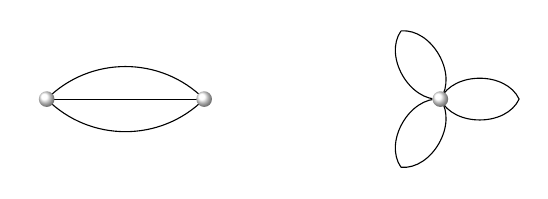
\begin{tikzpicture}[vertexBall, edgeStyle=nolabels, faceStyle=nolabels]
\coordinate (A) at (-1,0);
\coordinate (B) at (-3,0);
\coordinate (C) at (2,0);
%\coordinate (C1) at (2.7,-0.4);
%\coordinate (C2) at (1.3,-0.4);
%\coordinate (C3) at (2,1);
\coordinate (C1) at ( 1.5, 0.8660254037844387 );
\coordinate (C2) at ( 1.5, -0.8660254037844384 );
\coordinate (C3) at ( 3, 0 );

\draw[edge] (A) to[bend left=45] (B);
\draw[edge] (A) to[bend right=45] (B);
\draw[edge] (A) -- (B);

\draw[edge] (C) to[bend right=65] (C1);
\draw[edge] (C) to[bend left=65] (C1);
\draw[edge] (C) to[bend right=65] (C2);
\draw[edge] (C) to[bend left=65] (C2);
\draw[edge] (C) to[bend right=65] (C3);
\draw[edge] (C) to[bend left=65] (C3);
\vertexLabelR{A}{left}{};
\vertexLabelR{B}{left}{};
\vertexLabelR{C}{left}{};

                   \end{tikzpicture}
 

\end{center}
 

 For example the face graph of the one-face is given by a graph with one vertex
and three loops and the face graph of the Janus-Head is a graph with two
vertices which are connected through three edges. Note, the map resulting
through mapping a simplicial surface on it's face graph is not bijective,
since non-isomorphic surfaces can have isomorphic face graphs. But restricting
the map to spheres only delivers a bijection. We shall refer to two faces of a
simplicial surface as opposite if they share no common vertex. By looking at
the cube as an example, we see that the faces 1 and 6, 2 and 5, 3,4 form pairs
of opposite faces. 

 
\subsection{\textcolor{Chapter }{Face graph of a tetrahedron}}\label{Chapter_Tutorial_Section_Facegraph_of_simplicial_surfaces_Subsection_Face_graph_of_a_tetrahedron}
\logpage{[ 3, 2, 1 ]}
\hyperdef{L}{X7BB329EC7E5EB556}{}
{
  

 For the purpose of handling face graphs of simplicial we start with the
tetrahedron as an example. 

 
\begin{center}
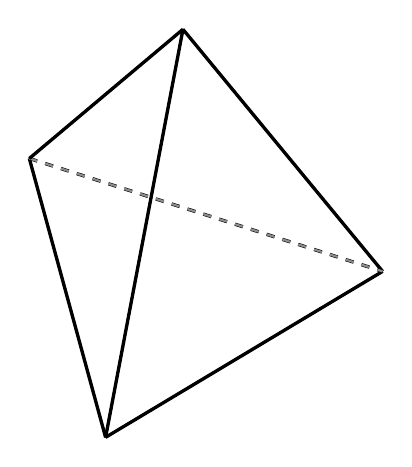
\begin{tikzpicture}[vertexBall, edgeDouble, faceStyle, scale=1]

\draw [edge=black] (-1.0314641277190677,-1.541558122060108)-- (2.4862868481518334,0.5659233184391239);
\draw [edge=black] (2.4862868481518334,0.5659233184391239)-- (-0.04902917049386102,3.639993991047026);
\draw [edge=black] (-0.04902917049386102,3.639993991047026)-- (-1.0314641277190677,-1.541558122060108);
\draw [edge=black] (-2,2)-- (-1.0314641277190677,-1.541558122060108);
\draw [dashed,edge] (-2,2)-- (2.4862868481518334,0.5659233184391239);
\draw [edge=black] (-2,2)-- (-0.04902917049386102,3.639993991047026);

\end{tikzpicture}

\end{center}
 

 Compute a tetrahedron 

 
\begin{Verbatim}[commandchars=!@|,fontsize=\small,frame=single,label=Example]
  !gapprompt@gap>| !gapinput@T:=Tetrahedron();|
  simplicial surface (4 vertices, 6 edges, and 4 faces)
\end{Verbatim}
 

 Define a function to compute the ordinal symbol of a simplicial surface 

 
\begin{Verbatim}[commandchars=!@|,fontsize=\small,frame=single,label=Example]
  !gapprompt@gap>| !gapinput@Symbol:=function(S)|
  !gapprompt@>| !gapinput@return [Size(Vertices(S)),Size(Edges(S)),Size(Faces(S))|
  ,VerticesOfEdges(S),EdgesOfFaces(S)];
  !gapprompt@>| !gapinput@end;|
  function( S ) ... end
\end{Verbatim}
 

 Compute the symbol of the Tetrahedron 

 
\begin{Verbatim}[commandchars=!@|,fontsize=\small,frame=single,label=Example]
  !gapprompt@gap>| !gapinput@Symbol(T);|
  [ 4, 6, 4, [ [ 1, 2 ], [ 1, 3 ], [ 1, 4 ], [ 2, 3 ], [ 2, 4 ], [ 3, 4 ] ], 
   [ [ 1, 2, 4 ], [ 1, 3, 5 ], [ 4, 5, 6 ], [ 2, 3, 6 ] ] ]
\end{Verbatim}
 

 Note, we can always replace a simplicial surface with n vertices, k edges and
m faces by an isomorphic surface where the set of vertices is given by [1..n],
the set of edges is given by [1..k] and the set of faces is given by [1..m] by
using the function CanonicalRepresentativeOfPolygonalSurface() 

 
\begin{Verbatim}[commandchars=!@|,fontsize=\small,frame=single,label=Example]
  !gapprompt@gap>| !gapinput@XX:=CanonicalRepresentativeOfPolygonalSurface(T);|
  [ simplicial surface (4 vertices, 6 edges, and 4 faces)
     , <polygonal morphism> ]
  !gapprompt@gap>| !gapinput@Symbol(XX[1]);|
  [ 4, 6, 4, [ [ 1, 2 ], [ 1, 3 ], [ 2, 3 ], [ 1, 4 ], [ 2, 4 ], [ 3, 4 ] ], 
   [ [ 1, 2, 3 ], [ 1, 4, 5 ], [ 2, 4, 6 ], [ 3, 5, 6 ] ] ]
\end{Verbatim}
 

 Compute the images of the vertices of T under the isomorphism mapping T on XX 

 
\begin{Verbatim}[commandchars=!@|,fontsize=\small,frame=single,label=Example]
  !gapprompt@gap>| !gapinput@List(Vertices(XX[1]),i->ImageOfVertex(XX[2],i));|
  [ 2, 1, 3, 4 ]
\end{Verbatim}
 

 We could do the same for the edges and faces, but since the vertices, etc are
already given by [1..4] etc. we shall continue our examinations with T. The
face graph can be constructed from the ordinal symbol of T We already know
that the set of vertices is given by the set of faces [1,2,3,4] and we can
compute the edges of the face graph by calling 

 
\begin{Verbatim}[commandchars=!@|,fontsize=\small,frame=single,label=Example]
  !gapprompt@gap>| !gapinput@FacesOfEdges(T);|
  [ [ 1, 2 ], [ 1, 4 ], [ 2, 4 ], [ 1, 3 ], [ 2, 3 ], [ 3, 4 ] ]
\end{Verbatim}
 

 Note, the edges of the face graph are also determined by the following list: 

 
\begin{Verbatim}[commandchars=!@|,fontsize=\small,frame=single,label=Example]
  !gapprompt@gap>| !gapinput@EdgesOfFaces(T);|
  [ [ 1, 2, 4 ], [ 1, 3, 5 ], [ 4, 5, 6 ], [ 2, 3, 6 ] ]
\end{Verbatim}
 

 
\begin{center}
            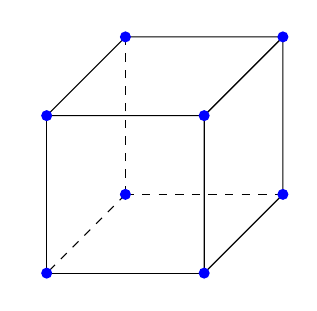
\begin{tikzpicture}[vertexStyle=nolabels, edgeStyle=nolabels]
                % We need to define the drawing style

                \coordinate (FDL) at (0,0); % front down left
                \coordinate (FDR) at (2,0); % front down right
                \coordinate (FUL) at (0,2); % front up left
                \coordinate (BDL) at (1,1); % back up left
                \coordinate (BDR) at ($(FDR)+(BDL)$); % back down right
                \coordinate (FUR) at ($(FUL)+(FDR)$); % front up right
                \coordinate (BUL) at ($(FUL)+(BDL)$); % back up left
                \coordinate (BUR) at ($(FDR)+(FUL)+(BDL)$); % back up right

                % Draw the edges
                \foreach \x in {FDL, BDR, BUL}{
                    \draw[dashed, edge] (BDL) -- (\x);
                }


                \draw[edge] (FDL) -- (FDR) -- (FUR) -- (FUL) -- cycle;
                \draw[edge] (FDR) -- (BDR) -- (BUR) -- (FUR) -- cycle;
                \draw[edge] (FUL) -- (FUR) -- (BUR) -- (BUL) -- cycle;

                % Draw the vertices
                \foreach \x in {FDL, FDR, FUL, BDL, BDR, FUR, BUL, BUR} {
                    \vertexLabelR{\x}{left}{}
                }
            \end{tikzpicture}


\end{center}
 

 Both lists are partual information of the ordinal symbol of the sphere. We
simply omitted the information for the vertices. But we can obtain the
vertices from the face graph closed edge-face-paths containing exactly three
faces and three edges. 

 
\begin{Verbatim}[commandchars=!@|,fontsize=\small,frame=single,label=Example]
  !gapprompt@gap>| !gapinput@VerticesOfEdges(T);|
  [ [ 1, 2 ], [ 1, 3 ], [ 1, 4 ], [ 2, 3 ], [ 2, 4 ], [ 3, 4 ] ]
  !gapprompt@gap>| !gapinput@UmbrellaPathsOfVertices(T);|
  [ ( e1, F1, e2, F4, e3, F2, e1 )
     , ( e1, F1, e4, F3, e5, F2, e1 )
     , ( e2, F1, e4, F3, e6, F4, e2 )
     , ( e3, F2, e5, F3, e6, F4, e3 ) 
  ]
\end{Verbatim}
 

 
\begin{center}
\input{tikzpictures/Image_FacegraphTetrahedron2.tex}
\end{center}
 

 Note, here the vertices are given in terms of edges and faces, i.e. only in
terms of the face graph. 

 Compute the corresponding closed edge-paths 

 
\begin{Verbatim}[commandchars=!@|,fontsize=\small,frame=single,label=Example]
  !gapprompt@gap>| !gapinput@List(last,r->EdgesAsList(r));|
  [ [ 1, 2, 3, 1 ], [ 1, 4, 5, 1 ], [ 2, 4, 6, 2 ], [ 3, 5, 6, 3 ] ]
\end{Verbatim}
 

 How can we reconstruct the VerticesOfEdges with knowledge of the face-graph?
Let the number of the vertices be encoded in the position of the closed paths
in the above list. So for example vertex 1 is incident to the edges 1, 2 and
3. This helps us to compute the desired set. 

 Furthermore define the function \texttt{Umbre2VeOfEd} which has a list of closed edge-face-paths as input and returns the
corresponding vertices of edges of a given surface. 

 
\begin{Verbatim}[commandchars=!@|,fontsize=\small,frame=single,label=Example]
  !gapprompt@gap>| !gapinput@Umbre2VeOfEd:=function(R)|
  !gapprompt@>| !gapinput@local L,ne,nv,i,j,rr;|
  !gapprompt@>| !gapinput@ne:=Size(Union(R));#Number of edges|
  !gapprompt@>| !gapinput@nv:=Size(R);#Number of vertices|
  !gapprompt@>| !gapinput@L:=List([1..ne],i->[]);|
  !gapprompt@>| !gapinput@for i in [1..nv] do|
  !gapprompt@>| !gapinput@for j in R[i] do|
  !gapprompt@>| !gapinput@L[j]:=Union(L[j],[i]);|
  !gapprompt@>| !gapinput@od;|
  !gapprompt@>| !gapinput@od;|
  !gapprompt@>| !gapinput@return L;|
  !gapprompt@>| !gapinput@end;|
  function( R ) ... end
\end{Verbatim}
 

 Now compute the vertices of edges of the tetrahedron \texttt{T} by using the function defined above 

 
\begin{Verbatim}[commandchars=!@|,fontsize=\small,frame=single,label=Example]
  !gapprompt@gap>| !gapinput@UmbrellaPathsOfVertices(T);|
  [ ( e1, F1, e2, F4, e3, F2, e1 )
     , ( e1, F1, e4, F3, e5, F2, e1 )
     , ( e2, F1, e4, F3, e6, F4, e2 )
     , ( e3, F2, e5, F3, e6, F4, e3 )
  ]
  !gapprompt@gap>| !gapinput@List(last,r->EdgesAsList(r));|
  [ [ 1, 2, 3, 1 ], [ 1, 4, 5, 1 ], [ 2, 4, 6, 2 ], [ 3, 5, 6, 3 ] ]
  !gapprompt@gap>| !gapinput@Umbre2VeOfEd(last);|
  [ [ 1, 2 ], [ 1, 3 ], [ 1, 4 ], [ 2, 3 ], [ 2, 4 ], [ 3, 4 ] ]
\end{Verbatim}
 

 Let us verify, that this set is indeed the vertices of edges of T 

 
\begin{Verbatim}[commandchars=!@|,fontsize=\small,frame=single,label=Example]
  !gapprompt@gap>| !gapinput@VerticesOfEdges(T);|
  [ [ 1, 2 ], [ 1, 3 ], [ 1, 4 ], [ 2, 3 ], [ 2, 4 ], [ 3, 4 ] ]
\end{Verbatim}
 Let us see whether there exists another simplicial surface \texttt{X} so that \texttt{X} and \texttt{T} have the same face graph. gap{\textgreater} \#T has 6 edges and hence contains
6 butterflies. The butterflies come gap{\textgreater} \#in pairs which have
the same boundary. This gives us a net of gap{\textgreater} \#three vertex
defining paths (why?) We want to examine the face that two non isomorphic
simplicial surfaces can have isomorphic face graphs. So we will construct a
simplicial surface which has the same face graph as our tetrahedron T. 

 Idea behind the construction 

 Since there exist 6 edges belonging to the sphere \texttt{T}, there are 6 butterflies contained in the tetrahedron. The butterflies can be
sorted into three pairs so that the two butterflies of the corresponding pair
of edges share the same boundary vertex-edge path. 

 
\begin{center}
\input{tikzpictures/Image_MultipleTetrahedron.tex}
\end{center}
 

 By interpreting the vertices of those paths as faces, we obtain three vertex
defining paths. 

 
\begin{Verbatim}[commandchars=!@|,fontsize=\small,frame=single,label=Example]
  !gapprompt@gap>| !gapinput@L:=List(Edges(T),r->Difference(Union(List(FacesOfEdge(T,r),f->EdgesOfFace(T,f))),[r]));|
  [ [ 2, 3, 4, 5 ], [ 1, 3, 4, 6 ], [ 1, 2, 5, 6 ], [ 1, 2, 5, 6 ], 
   [ 1, 3, 4, 6 ], [ 2, 3, 4, 5 ] ]
  !gapprompt@gap>| !gapinput@L:=Set(L);|
  [ [ 1, 2, 5, 6 ], [ 1, 3, 4, 6 ], [ 2, 3, 4, 5 ] ]
  !gapprompt@gap>| !gapinput@Umbre2VeOfEd(last);|
  [ [ 1, 2 ], [ 1, 3 ], [ 2, 3 ], [ 2, 3 ], [ 1, 3 ], [ 1, 2 ] ]
  !gapprompt@gap>| !gapinput@nn:=last;;|
\end{Verbatim}
 

 Note that the elements of L are not stricly paths but the sets of edges that
occur in a relevant path. But that is enough for our purpose of constructing
the desired simplicial surface. 

 
\begin{Verbatim}[commandchars=!@|,fontsize=\small,frame=single,label=Example]
  !gapprompt@gap>| !gapinput@TT:=PolygonalComplexByDownwardIncidence(nn,EdgesOfFaces(T));|
  simplicial surface (3 vertices, 6 edges, and 4 faces)
  !gapprompt@gap>| !gapinput@EulerCharacteristic(TT);|
  1
  !gapprompt@gap>| !gapinput@IsOrientable(TT);|
  false
\end{Verbatim}
 

 Since the Euler-Characteristic of the surfaces differ and the constructed
surface is not orientable it cannot be isomorphic to an tetrahedron 

 Of course it would be desiralbe to compute all simplicial surfaces having the
same face graph up to isomorphism. 

 }

 
\subsection{\textcolor{Chapter }{Face graph of an octahedron}}\label{Chapter_Tutorial_Section_Facegraph_of_simplicial_surfaces_Subsection_Face_graph_of_an_octahedron}
\logpage{[ 3, 2, 2 ]}
\hyperdef{L}{X7B3EBE2781DD2666}{}
{
  

 Let us analyse the face graph of an octahedron as second example. 

 
\begin{Verbatim}[commandchars=!@|,fontsize=\small,frame=single,label=Example]
  !gapprompt@gap>| !gapinput@ok:=Octahedron();|
  simplicial surface (6 vertices, 12 edges, and 8 faces)
\end{Verbatim}
 

 Compute the octahedron's symbol 

 
\begin{Verbatim}[commandchars=!@|,fontsize=\small,frame=single,label=Example]
  !gapprompt@gap>| !gapinput@Symbol(ok);|
  [ 6, 12, 8, 
   [ [ 1, 2 ], [ 1, 3 ], [ 1, 4 ], [ 1, 5 ], [ 2, 3 ], [ 2, 5 ], [ 2, 6 ], 
       [ 3, 4 ], [ 3, 6 ], [ 4, 5 ], [ 4, 6 ], [ 5, 6 ] ], 
   [ [ 1, 2, 5 ], [ 6, 7, 12 ], [ 1, 4, 6 ], [ 5, 7, 9 ], [ 3, 4, 10 ], 
       [ 8, 9, 11 ], [ 2, 3, 8 ], [ 10, 11, 12 ] ] ]
  !gapprompt@gap>| !gapinput@okc:=FacesOfEdges(ok);|
  [ [ 1, 3 ], [ 1, 7 ], [ 5, 7 ], [ 3, 5 ], [ 1, 4 ], [ 2, 3 ], [ 2, 4 ], 
   [ 6, 7 ], [ 4, 6 ], [ 5, 8 ], [ 6, 8 ], [ 2, 8 ] ]
\end{Verbatim}
 

 
\begin{center}
\input{tikzpictures/Image_FacegraphOfOctahedron.tex}
\end{center}
 

 Note the edge graph of a simplicial surface is the graph resulting from the
vertices and edges of the surfaces being the vertices and edges of the graph.
Two vertices V1,V2 connected through an edge in the graph if they are incident
vertices in the surface. The face graph of an octahedron is isomorphic to the
edge graph of a cube. 

 
\begin{center}
            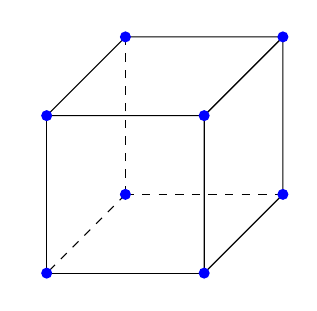
\begin{tikzpicture}[vertexStyle=nolabels, edgeStyle=nolabels]
                % We need to define the drawing style

                \coordinate (FDL) at (0,0); % front down left
                \coordinate (FDR) at (2,0); % front down right
                \coordinate (FUL) at (0,2); % front up left
                \coordinate (BDL) at (1,1); % back up left
                \coordinate (BDR) at ($(FDR)+(BDL)$); % back down right
                \coordinate (FUR) at ($(FUL)+(FDR)$); % front up right
                \coordinate (BUL) at ($(FUL)+(BDL)$); % back up left
                \coordinate (BUR) at ($(FDR)+(FUL)+(BDL)$); % back up right

                % Draw the edges
                \foreach \x in {FDL, BDR, BUL}{
                    \draw[dashed, edge] (BDL) -- (\x);
                }


                \draw[edge] (FDL) -- (FDR) -- (FUR) -- (FUL) -- cycle;
                \draw[edge] (FDR) -- (BDR) -- (BUR) -- (FUR) -- cycle;
                \draw[edge] (FUL) -- (FUR) -- (BUR) -- (BUL) -- cycle;

                % Draw the vertices
                \foreach \x in {FDL, FDR, FUL, BDL, BDR, FUR, BUL, BUR} {
                    \vertexLabelR{\x}{left}{}
                }
            \end{tikzpicture}


\end{center}
 

 The vertices of the octahedron are determined by the closed paths containing
exactly four faces and edges. 

 
\begin{Verbatim}[commandchars=!@|,fontsize=\small,frame=single,label=Example]
  !gapprompt@gap>| !gapinput@UmbrellaPathsOfVertices(ok);|
  [ ( e1, F1, e2, F7, e3, F5, e4, F3, e1 )
     , ( 1, F1, e5, F4, e7, F2, e6, F3, e1 )
     , ( e2, F1, e5, F4, e9, F6, e8, F7, e2 )
     , ( e3, F5, e10, F8, e11, F6, e8, F7, e3 )
     , ( e4, F3, e6, F2, e12, F8, e10, F5, e4 )
     ,  ( e7, F2, e12, F8, e11, F6, e9, F4, e7) 
  ]
  !gapprompt@gap>| !gapinput@List(last,r->EdgesAsList(r));|
  [ [ 1, 2, 3, 4, 1 ], [ 1, 5, 7, 6, 1 ], [ 2, 5, 9, 8, 2 ], 
   [ 3, 10, 11, 8, 3 ], [ 4, 6, 12, 10, 4 ], [ 7, 12, 11, 9, 7 ] ]
  !gapprompt@gap>| !gapinput@List(last2,r->FacesAsList(r));|
  [ [ 1, 7, 5, 3 ], [ 1, 4, 2, 3 ], [ 1, 4, 6, 7 ], [ 5, 8, 6, 7 ], 
    [ 3, 2, 8, 5 ], [ 2, 8, 6, 4 ] ]
\end{Verbatim}
 

 Compute the opposite faces of the octahedron ok 

 
\begin{Verbatim}[commandchars=!@|,fontsize=\small,frame=single,label=Example]
  !gapprompt@gap>| !gapinput@VV:=VerticesOfFaces(ok);|
  [ [ 1, 2, 3 ], [ 2, 5, 6 ], [ 1, 2, 5 ], [ 2, 3, 6 ], [ 1, 4, 5 ], 
   [ 3, 4, 6 ], [ 1, 3, 4 ], [ 4, 5, 6 ] ]
  !gapprompt@gap>| !gapinput@List([1..8],i->Filtered([1..8],r->Intersection(VV[i],VV[r])=[]));|
  [ [ 8 ], [ 7 ], [ 6 ], [ 5 ], [ 4 ], [ 3 ], [ 2 ], [ 1 ] ]
\end{Verbatim}
 

 Hence the pairs of opposite faces are [1,8], [2,7], [3,6] and [4,5].
gap{\textgreater} \# Those vertex-edge-paths avoiding the vertices of such a
diagonal gap{\textgreater} \# are all in one dihedral class. Taken together
they correspond to the vertices of gap{\textgreater} \# of a surface in the
same edge-face-class as ok: 

 
\begin{Verbatim}[commandchars=!@|,fontsize=\small,frame=single,label=Example]
  !gapprompt@gap>| !gapinput@List([1,8],i->EdgesOfFace(ok,i));|
  [ [ 1, 2, 5 ], [ 10, 11, 12 ] ]
  !gapprompt@gap>| !gapinput@z1:=Difference(Edges(ok),Union(last));|
  [ 3, 4, 6, 7, 8, 9 ]
  !gapprompt@gap>| !gapinput@List([2,7],i->EdgesOfFace(ok,i));|
  [ [ 6, 7, 12 ], [ 2, 3, 8 ] ]
  !gapprompt@gap>| !gapinput@z2:=Difference(Edges(ok),Union(last));|
  [ 1, 4, 5, 9, 10, 11 ]
  !gapprompt@gap>| !gapinput@List([3,6],i->EdgesOfFace(ok,i));|
  [ [ 1, 4, 6 ], [ 8, 9, 11 ] ]
  !gapprompt@gap>| !gapinput@z3:=Difference(Edges(ok),Union(last));|
  [ 2, 3, 5, 7, 10, 12 ]
  !gapprompt@gap>| !gapinput@List([4,5],i->EdgesOfFace(ok,i));|
  [ [ 5, 7, 9 ], [ 3, 4, 10 ] ]
  !gapprompt@gap>| !gapinput@z4:=Difference(Edges(ok),Union(last));|
  [ 1, 2, 6, 8, 11, 12 ]
  !gapprompt@gap>| !gapinput@Umbre2VeOfEd([z1,z2,z3,z4]);|
  [ [ 2, 4 ], [ 3, 4 ], [ 1, 3 ], [ 1, 2 ], [ 2, 3 ], [ 1, 4 ], [ 1, 3 ], 
    [ 1, 4 ], [ 1, 2 ], [ 2, 3 ], [ 2, 4 ], [ 3, 4 ] ]
  !gapprompt@gap>| !gapinput@nok:=PolygonalComplexByDownwardIncidence(last,EdgesOfFaces(ok));|
  simplicial surface (4 vertices, 12 edges, and 8 faces)
\end{Verbatim}
 

 Compute elementary to verify that nok is not isomorphic to the octahedron ok 

 
\begin{Verbatim}[commandchars=!@|,fontsize=\small,frame=single,label=Example]
  !gapprompt@gap>| !gapinput@EulerCharacteristic(nok);|
  0
  !gapprompt@gap>| !gapinput@VertexCounter(nok);|
  [ [ 6, 4 ] ]
  !gapprompt@gap>| !gapinput@IsOrientable(nok);|
  true
\end{Verbatim}
 

 gap{\textgreater} \#Hence it is a torus. One can easily recover it from a
hexagonal gap{\textgreater} \#in the plane by cutting out a rhombus of
appropriate size and gap{\textgreater} \#identify opposite sides. A nice
challenge in paperfolding: gap{\textgreater} \#Embed the barycentric
subdivision of this gadget into 3-space in gap{\textgreater} \#such a way that
all the smaller triangles lie in one plane. gap{\textgreater}
gap{\textgreater} \#We finish this worksheet by visalizing TT, the projective
plane above. 

 
\begin{Verbatim}[commandchars=!@|,fontsize=\small,frame=single,label=Example]
  !gapprompt@gap>| !gapinput@TT;|
  simplicial surface (3 vertices, 6 edges, and 4 faces)
  !gapprompt@gap>| !gapinput@IsOrientable(TT);|
  false
  !gapprompt@gap>| !gapinput@EulerCharacteristic(TT);|
  1
\end{Verbatim}
 

 gap{\textgreater} \#We shall construct a 2-fold covering of TT by the
octahedron 

 
\begin{Verbatim}[commandchars=!@|,fontsize=\small,frame=single,label=Example]
  !gapprompt@gap>| !gapinput@VertexCounter (TT);|
  [ [ 4, 3 ] ]
  !gapprompt@gap>| !gapinput@AutomorphismGroup(TT);|
  Group([ (1,2)(5,6)(7,8)(10,11), (1,2)(5,7)(6,8)(12,13), (2,3)(4,5)(8,9)
  (11,13) ])
  !gapprompt@gap>| !gapinput@StructureDescription(last);|
  "S4"
  !gapprompt@gap>| !gapinput@G:=AutomorphismGroup(ok);|
  Group([ (1,2)(4,6)(8,11)(9,13)(10,12)(14,15)(16,18)(20,23)(22,25), (3,5)
  (8,10)(11,12)(14,16)(15,18)(19,21)(20,22)(23,25)(24,26), (2,3)(4,5)(7,8)
  (9,10)(12,14)(13,15)(17,18)(20,24)(21,25) ])
  !gapprompt@gap>| !gapinput@StructureDescription(G);|
  "C2 x S4"
  !gapprompt@gap>| !gapinput@C:=Center(G);|
  Group([ (1,6)(2,4)(3,5)(7,17)(8,18)(9,13)(10,15)(11,16)(12,14)(19,26)(20,25)
  (21,24)(22,23) ])
  !gapprompt@gap>| !gapinput@Orbits(C,Vertices(ok));|
  [ [ 1, 6 ], [ 2, 4 ], [ 3, 5 ] ]
  !gapprompt@gap>| !gapinput@Orbits(C,Edges(ok));|
  [ [ 1, 6 ], [ 2, 4 ], [ 3, 5 ], [ 7, 17 ], [ 8, 18 ], [ 9, 13 ], [ 10, 15 ], 
   [ 11, 16 ], [ 12, 14 ] ]
\end{Verbatim}
 

 gap{\textgreater} \#The numbering gets confusing. We do edges and faces by
themselves each 

 
\begin{Verbatim}[commandchars=!@|,fontsize=\small,frame=single,label=Example]
  !gapprompt@gap>| !gapinput@Ge:=AutomorphismGroupOnEdges(ok);|
  Group([ (2,5)(3,7)(4,6)(8,9)(10,12), (2,4)(5,6)(8,10)(9,12), (1,2)(3,4)(6,8)
  (7,9)(11,12) ])
  !gapprompt@gap>| !gapinput@Ce:=Center(Ge);|
  Group([ (1,11)(2,12)(3,7)(4,9)(5,10)(6,8) ])
  !gapprompt@gap>| !gapinput@Orbits(Ge,Edges(ok));|
  [ [ 1, 2, 5, 4, 6, 3, 8, 7, 9, 10, 12, 11 ] ]
  !gapprompt@gap>| !gapinput@Orbits(Ce,Edges(ok));|
  [ [ 1, 11 ], [ 2, 12 ], [ 3, 7 ], [ 4, 9 ], [ 5, 10 ], [ 6, 8 ] ]
  !gapprompt@gap>| !gapinput@Gf:=AutomorphismGroupOnFaces(ok);|
  Group([ (2,5)(4,7), (1,3)(2,4)(5,7)(6,8), (2,6)(3,7) ])
  !gapprompt@gap>| !gapinput@Cf:=Center(Gf);|
  Group([ (1,8)(2,7)(3,6)(4,5) ])
  !gapprompt@gap>| !gapinput@Fo:=Orbits(Cf,Faces(ok));|
  [ [ 1, 8 ], [ 2, 7 ], [ 3, 6 ], [ 4, 5 ] ]
  !gapprompt@gap>| !gapinput@Eo:=Orbits(Ce,Edges(ok));|
  [ [ 1, 11 ], [ 2, 12 ], [ 3, 7 ], [ 4, 9 ], [ 5, 10 ], [ 6, 8 ] ]
  !gapprompt@gap>| !gapinput@Vo:=Orbits(C,Vertices(ok));|
  [ [ 1, 6 ], [ 2, 4 ], [ 3, 5 ] ]
  !gapprompt@gap>| !gapinput@List([1,2,3],i->EdgesOfFace(ok,i));|
  [ [ 1, 2, 5 ], [ 6, 7, 12 ], [ 1, 4, 6 ] ]
  !gapprompt@gap>| !gapinput@List([6,4,5],i->EdgesOfFace(ok,i));|
  [ [ 8, 9, 11 ], [ 5, 7, 9 ], [ 3, 4, 10 ] ]
  !gapprompt@gap>| !gapinput@Eo;|
  [ [ 1, 11 ], [ 2, 12 ], [ 3, 7 ], [ 4, 9 ], [ 5, 10 ], [ 6, 8 ] ]
  !gapprompt@gap>| !gapinput@Fo;|
  [ [ 1, 8 ], [ 2, 7 ], [ 3, 6 ], [ 4, 5 ] ]
  !gapprompt@gap>| !gapinput@List([1,2,3,4],i->EdgesOfFace(ok,i));|
  [ [ 1, 2, 5 ], [ 6, 7, 12 ], [ 1, 4, 6 ], [ 5, 7, 9 ] ]
  !gapprompt@gap>| !gapinput@List([8,7,6,5],i->EdgesOfFace(ok,i));|
  [ [ 10, 11, 12 ], [ 2, 3, 8 ], [ 8, 9, 11 ], [ 3, 4, 10 ] ]
  !gapprompt@gap>| !gapinput@Eo;|
  [ [ 1, 11 ], [ 2, 12 ], [ 3, 7 ], [ 4, 9 ], [ 5, 10 ], [ 6, 8 ] ]
  !gapprompt@gap>| !gapinput@EoF:=[[1,2,5],[2,3,6],[1,4,6],[3,4,5]];|
  [ [ 1, 2, 5 ], [ 2, 3, 6 ], [ 1, 4, 6 ], [ 3, 4, 5 ] ]
\end{Verbatim}
 

 gap{\textgreater} \#Now the vertices of Edges: 

 
\begin{Verbatim}[commandchars=!@|,fontsize=\small,frame=single,label=Example]
  !gapprompt@gap>| !gapinput@Eo;|
  [ [ 1, 11 ], [ 2, 12 ], [ 3, 7 ], [ 4, 9 ], [ 5, 10 ], [ 6, 8 ] ]
  !gapprompt@gap>| !gapinput@Eo1:=List(Eo,i->i[1]);|
  [ 1, 2, 3, 4, 5, 6 ]
  !gapprompt@gap>| !gapinput@Eo2:=List(Eo,i->i[2]);|
  [ 11, 12, 7, 9, 10, 8 ]
  !gapprompt@gap>| !gapinput@List(Eo1,i->VerticesOfEdge(ok,i));|
  [ [ 1, 2 ], [ 1, 3 ], [ 1, 4 ], [ 1, 5 ], [ 2, 3 ], [ 2, 5 ] ]
  !gapprompt@gap>| !gapinput@List(Eo2,i->VerticesOfEdge(ok,i));|
  [ [ 4, 6 ], [ 5, 6 ], [ 2, 6 ], [ 3, 6 ], [ 4, 5 ], [ 3, 4 ] ]
  !gapprompt@gap>| !gapinput@Vo;|
  [ [ 1, 6 ], [ 2, 4 ], [ 3, 5 ] ]
  !gapprompt@gap>| !gapinput@VoE:=[[1,2],[1,3],[1,2],[1,3],[2,3],[2,3]];|
  [ [ 1, 2 ], [ 1, 3 ], [ 1, 2 ], [ 1, 3 ], [ 2, 3 ], [ 2, 3 ] ]
  !gapprompt@gap>| !gapinput@Okmod:=PolygonalComplexByDownwardIncidence(VoE,EoF);|
  simplicial surface (3 vertices, 6 edges, and 4 faces)
  !gapprompt@gap>| !gapinput@IsIsomorphic(Okmod,TT);|
  true
\end{Verbatim}
 }

 }

 
\section{\textcolor{Chapter }{Vertex-faithful surfaces}}\label{Section_vertex-faithful_surfaces}
\logpage{[ 3, 3, 0 ]}
\hyperdef{L}{X7E4C8F597DDDBAB2}{}
{
  

 $Problems:$ 
\begin{itemize}
\item  Construction of multi-tetrahedral spheres 
\end{itemize}
 $Theoretical$ $background$ 
\begin{itemize}
\item  Vertex-faithful surfaces and boolean operations 
\end{itemize}
 $Frequently$ $used$ $commands$ 
\begin{itemize}
\item  AllSimplicialSpheres() (\ref{AllSimplicialSpheres}) 
\item  AutomorphismGroupOnEdges() (\ref{AutomorphismGroupOnEdges}) 
\item  AutomorphismGroupOnFaces() (\ref{AutomorphismGroupOnFaces}) 
\item  EdgesOfFaces() (local version: EdgesOfFace()) (\ref{EdgesOfFaces}) 
\item  EdgesOfVertices() (local version: Edges) (\ref{EdgesOfVertices}) 
\item  FaceDegreesOfVertices() (local version: FaceDegreeOfVertex)(\ref{FaceDegreesOfVertices}) 
\item  FacesOfEdges() (local version: FacesOfEdge()) (\ref{FacesOfEdges}) 
\item  IsIsomorphic() (\ref{IsIsomorphic}) 
\item  SimplicialSurfaceByVerticesInFaces() (works for vertex-faithful surfaces only)
(\ref{PolygonalStructures_surface}) 
\item  VertexCounter() (local version: DegreeOfVertex()) (\ref{VertexCounter}), 
\item  VerticesOfFaces() (local Version: VerticesOfFace()) (\ref{VerticesOfFaces}) 
\end{itemize}
 $Less$ $frequently$ $used$ $commands$ 
\begin{itemize}
\item  Tetrahedron() (\ref{Tetrahedron}) 
\end{itemize}
 

 $ Mathematical$ $details:$ 

 This section deals with vertex-faithful surfaces. A simplicial surface is
vertex-faithful if and only if the map resulting by mapping an edge resp. face
on it's set of incident vertices is injective. An example of a non
vertex-faithful sphere is the Janus-Head. 

 
\begin{center}


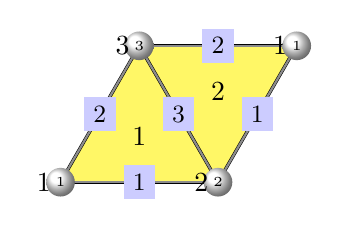
\begin{tikzpicture}[vertexBall, edgeDouble, faceStyle, scale=2]

% Define the coordinates of the vertices
\coordinate (V1_1) at (0, 0);
\coordinate (V2_1) at (1, 0);
\coordinate (V3_1) at (0.5, 0.8660254037844386);
\coordinate (V4_1) at (1.5, 0.8660254037844386);


% Fill in the faces
\fill[face]  (V2_1) -- (V3_1) -- (V1_1) -- cycle;
\node[faceLabel] at (barycentric cs:V2_1=1,V3_1=1,V1_1=1) {$1$};
\fill[face]  (V2_1) -- (V4_1) -- (V3_1) -- cycle;
\node[faceLabel] at (barycentric cs:V2_1=1,V4_1=1,V3_1=1) {$2$};


% Draw the edges
\draw[edge] (V2_1) -- node[edgeLabel] {$1$} (V1_1);
\draw[edge] (V1_1) -- node[edgeLabel] {$2$} (V3_1);
\draw[edge] (V3_1) -- node[edgeLabel] {$3$} (V2_1);
\draw[edge] (V4_1) -- node[edgeLabel] {$1$} (V2_1);
\draw[edge] (V3_1) -- node[edgeLabel] {$2$} (V4_1);


% Draw the vertices
\vertexLabelR{V1_1}{left}{$1$}
\vertexLabelR{V2_1}{left}{$2$}
\vertexLabelR{V3_1}{left}{$3$}
\vertexLabelR{V4_1}{left}{$1$}

\end{tikzpicture}

\end{center}
 

 
\begin{Verbatim}[commandchars=!@|,fontsize=\small,frame=single,label=Example]
  !gapprompt@gap>| !gapinput@JanusHead();|
  simplicial surface (3 vertices, 3 edges, and 2 faces)
  !gapprompt@gap>| !gapinput@VerticesOfFaces(last);|
  [ [ 1, 2, 3 ], [ 1, 2, 3 ] ]
\end{Verbatim}
 

 In this exercise we construct multi-tetrahedral spheres. A multi-tetrahedral
sphere is a vertex-faithful sphere constructed through tetrahedral extensions.
Starting from a tetrahedron we iteratively replace faces by 3-gons to obtain
the desired spheres. We have already seen examples of multi-tetrahedral
spheres, namely the tetrahedron and the double-tetrahedron. 

 
\begin{center}
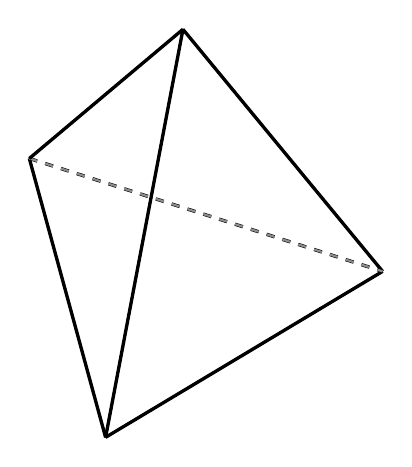
\begin{tikzpicture}[vertexBall, edgeDouble, faceStyle, scale=1]

\draw [edge=black] (-1.0314641277190677,-1.541558122060108)-- (2.4862868481518334,0.5659233184391239);
\draw [edge=black] (2.4862868481518334,0.5659233184391239)-- (-0.04902917049386102,3.639993991047026);
\draw [edge=black] (-0.04902917049386102,3.639993991047026)-- (-1.0314641277190677,-1.541558122060108);
\draw [edge=black] (-2,2)-- (-1.0314641277190677,-1.541558122060108);
\draw [dashed,edge] (-2,2)-- (2.4862868481518334,0.5659233184391239);
\draw [edge=black] (-2,2)-- (-0.04902917049386102,3.639993991047026);

\end{tikzpicture}

\end{center}
 

 In this exercise we shall refer to a vertex of face degree 3 together with
it's incident faces and edges as tetrahedron. Furthermore we say that a
tetrahedron is attached resp. a tetrahedron is removed, if we replace a face
by a 3-gon resp. a 3-gon by a face. 

 
\begin{center}
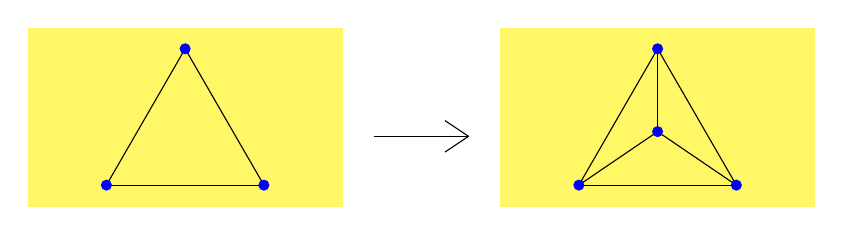
\begin{tikzpicture}[vertexBall, edgeDouble, faceStyle, scale=2, edgeStyle=nolabels,vertexStyle=nolabels]
\coordinate (V1) at (-1.5, 0.8660254037844386);
\coordinate (V2) at (-1, 0);
\coordinate (V3) at (-2, 0);
\coordinate (V4) at (1.5, 0.8660254037844386);
\coordinate (V5) at (1, 0);
\coordinate (V6) at (2, 0);
\coordinate (V7) at (1.5, 0.34);

\fill[face]  (0.5,-0.14) -- (2.5,-0.14) -- (2.5,1) -- (0.5,1) -- cycle;
\fill[face]  (-0.5,-0.14) -- (-2.5,-0.14) -- (-2.5,1) -- (-0.5,1) -- cycle;

\draw[edge=black] (-0.3,0.31) -- (0.3,0.31);
\draw[edge=black] (0.15,0.41) -- (0.3,0.31);
\draw[edge=black] (0.15,0.21) -- (0.3,0.31);
\draw[edge=black] (V1) -- (V2);
\draw[edge=black] (V2) -- (V3);
\draw[edge=black] (V1) -- (V3);
\draw[edge=black] (V4) -- (V5);
\draw[edge=black] (V5) -- (V6);
\draw[edge=black] (V4) -- (V6);
\draw[edge=black] (V4) -- (V7);
\draw[edge=black] (V5) -- (V7);
\draw[edge=black] (V6) -- (V7);

\vertexLabelR{V1}{left}{}
\vertexLabelR{V2}{left}{}
\vertexLabelR{V3}{left}{}
\vertexLabelR{V4}{left}{}
\vertexLabelR{V5}{left}{}
\vertexLabelR{V6}{left}{}
\vertexLabelR{V7}{left}{}
\end{tikzpicture}

\end{center}
 

 We can construct a new sphere out of a vertex-faithful sphere by removing all
attached tetrahedra. So in other words, a vertex-faithful sphere is a
multi-tetrahedral sphere if and only if iteratively removing all tetrahedra
from the constructed spheres leads to the tetrahedron or the
double-tetrahedron. Since we are only interested in surfaces we shall refer to
terms like tetrahedron, double- tetrahedron, etc. as the combinatorial devices
describing their combinatorial structure. So we will work with their incidence
geometry and view them as abstract surfaces. Note, constructing a new sphere
by replacing a face by a tetrahedron can be seen as a subdivision of a
surface. 

 
\subsection{\textcolor{Chapter }{Multi-tetrahedral spheres}}\label{Chapter_Tutorial_Section_Vertex-faithful_surfaces_Subsection_Multi-tetrahedral_spheres}
\logpage{[ 3, 3, 1 ]}
\hyperdef{L}{X86EE109F87BCE7F9}{}
{
  

 $Idea$ $behind$ $the$ $construcion$ 

 We construct multi-tetrahedral spheres with up to 12 faces by using their sets
of vertices in faces. Tetrahedral extensions can be achieved by computing the
symmetric difference of a given multi-tetrahedral sphere and a tetrahedron,
both represented by their vertices in faces. Note, although spheres are
constructed by replacing different faces of a sphere by tetrahedra, the
resulting spheres can still be isomorphic. 

 
\begin{Verbatim}[commandchars=!@|,fontsize=\small,frame=single,label=Example]
  !gapprompt@gap>| !gapinput@t1:=Combinations([1,2,3,4],3);|
  [ [ 1, 2, 3 ], [ 1, 2, 4 ], [ 1, 3, 4 ], [ 2, 3, 4 ] ]
  !gapprompt@gap>| !gapinput@T:=SimplicialSurfaceByVerticesInFaces(t1);|
  simplicial surface (4 vertices, 6 edges, and 4 faces)
\end{Verbatim}
 

 
\begin{center}
\input{tikzpictures/Image_Tetrahedron.tex}
\end{center}
 

 Replace face [2,3,4] by a tetrahedron 

 
\begin{Verbatim}[commandchars=!@|,fontsize=\small,frame=single,label=Example]
  !gapprompt@gap>| !gapinput@t11:=Combinations([2,3,4,5],3);|
  [ [ 2, 3, 4 ], [ 2, 3, 5 ], [ 2, 4, 5 ], [ 3, 4, 5 ] ]
  !gapprompt@gap>| !gapinput@Sydi(t1,t11);|
  [ [ 1, 2, 3 ], [ 1, 2, 4 ], [ 1, 3, 4 ], [ 2, 3, 5 ],
    [ 2, 4, 5 ], [ 3, 4, 5 ] ]
  !gapprompt@gap>| !gapinput@T11:=SimplicialSurfaceByVerticesInFaces(last);|
  simplicial surface (5 vertices, 9 edges, and 6 faces)
\end{Verbatim}
 

 Replace face [1,2,3] by a tetrahedron 

 
\begin{Verbatim}[commandchars=!@|,fontsize=\small,frame=single,label=Example]
  !gapprompt@gap>| !gapinput@t12:=Combinations([1,2,3,5],3);|
  [ [ 1, 2, 3 ], [ 1, 2, 5 ], [ 1, 3, 5 ], [ 2, 3, 5 ] ]
  !gapprompt@gap>| !gapinput@Sydi(t1,t12);|
  [ [ 1, 2, 4 ], [ 1, 3, 4 ], [ 2, 3, 4 ], [ 1, 2, 5 ],
    [ 1, 3, 5 ], [ 2, 3, 5 ] ]
  !gapprompt@gap>| !gapinput@T12:=SimplicialSurfaceByVerticesInFaces(last);|
  simplicial surface (5 vertices, 9 edges, and 6 faces)
\end{Verbatim}
 

 Replace face [1,2,4] by a tetrahedron 

 
\begin{Verbatim}[commandchars=!@|,fontsize=\small,frame=single,label=Example]
  !gapprompt@gap>| !gapinput@t13:=Combinations([1,2,4,5],3);|
  [ [ 1, 2, 4 ], [ 1, 2, 5 ], [ 1, 4, 5 ], [ 2, 4, 5 ] ]
  !gapprompt@gap>| !gapinput@Sydi(t1,t13);|
  [ [ 1, 2, 3 ], [ 1, 3, 4 ], [ 2, 3, 4 ], [ 1, 2, 5 ],
    [ 1, 4, 5 ], [ 2, 4, 5 ] ]
  !gapprompt@gap>| !gapinput@T13:=SimplicialSurfaceByVerticesInFaces(last);|
  simplicial surface (5 vertices, 9 edges, and 6 faces)
\end{Verbatim}
 

 Replace face [1,3,4] by a tetrahedron 

 
\begin{Verbatim}[commandchars=!@|,fontsize=\small,frame=single,label=Example]
  !gapprompt@gap>| !gapinput@t14:=Combinations([1,3,4,5],3);|
  [ [ 1, 3, 4 ], [ 1, 3, 5 ], [ 1, 4, 5 ], [ 3, 4, 5 ] ]
  !gapprompt@gap>| !gapinput@Sydi(t1,t14);|
  [ [ 1, 2, 3 ], [ 1, 2, 4 ], [ 2, 3, 4 ], [ 1, 3, 5 ],
    [ 1, 4, 5 ], [ 3, 4, 5 ] ]
  !gapprompt@gap>| !gapinput@T14:=SimplicialSurfaceByVerticesInFaces(last);|
  simplicial surface (5 vertices, 9 edges, and 6 faces)
\end{Verbatim}
 

 Check whether the constructed surfaces are isomorphic 

 
\begin{Verbatim}[commandchars=!@|,fontsize=\small,frame=single,label=Example]
  !gapprompt@gap>| !gapinput@List([T12,T13,T14],S->IsIsomorphic(T11,S));|
  [ true, true, true ]
\end{Verbatim}
 

 
\begin{center}
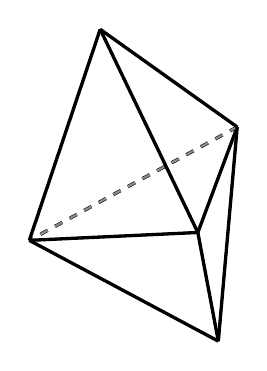
\begin{tikzpicture}[edgeDouble, scale=1]

\draw [edge=black] (0.64,-2.14)-- (1.14,-0.8);

\draw [edge,dashed] (1.14,-0.8)-- (-1.5,-2.24);

\draw [edge=black] (-1.5,-2.24)-- (0.64,-2.14);

\draw [edge=black] (-0.6,0.44)-- (1.14,-0.8);

\draw [edge=black] (-0.6,0.44)-- (0.64,-2.14);

\draw [edge=black] (-0.6,0.44)-- (-1.5,-2.24);

\draw [edge=black] (-1.5,-2.24)-- (0.9,-3.52);

\draw [edge=black] (0.9,-3.52)-- (0.64,-2.14);

\draw [edge=black] (0.9,-3.52)-- (1.14,-0.8);

\end{tikzpicture}



\end{center}
 

 So special care has to be taken to the choice of faces. Furthermore we
introduce some terminology for the purpose of having an easy way to refer to
the constructed spheres. Let X be a multi-tetrahedral sphere. We shall refer
to surfaces obtained through a tetrahedral extension on X as children of X. So
the double-tetrahedron is a child of the tetrahedron. 

 Start by defining the function \texttt{Te()} which returns the set of vertices in faces of a tetrahedron whereby the four
vertices are given by \texttt{a,b,c,d} 

 
\begin{Verbatim}[commandchars=!@|,fontsize=\small,frame=single,label=Example]
  !gapprompt@gap>| !gapinput@Te:=function(a,b,c,d)|
  !gapprompt@>| !gapinput@return Combinations([a,b,c,d],3);|
  !gapprompt@>| !gapinput@end;|
  function( a, b, c, d ) ... end
\end{Verbatim}
 

 Up to isomorphism there is exactly one multi-tetrahedral sphere with 4 faces.
Compute the vertices in faces of the first tetrahedron T1: 

 
\begin{center}
\input{tikzpictures/Image_Tetrahedron.tex}
\end{center}
 
\begin{Verbatim}[commandchars=!@|,fontsize=\small,frame=single,label=Example]
  !gapprompt@gap>| !gapinput@T1:=Te(1,2,3,4);|
  [ [ 1, 2, 3 ], [ 1, 2, 4 ], [ 1, 3, 4 ], [ 2, 3, 4 ] ]
  !gapprompt@gap>| !gapinput@VerticesOfFaces(Tetrahedron());|
  [ [ 1, 2, 3 ], [ 1, 2, 4 ], [ 2, 3, 4 ], [ 1, 3, 4 ] ]
  !gapprompt@gap>| !gapinput@Te(2,3,4,5);|
  [ [ 2, 3, 4 ], [ 2, 3, 5 ], [ 2, 4, 5 ], [ 3, 4, 5 ] ]
\end{Verbatim}
 

 As seen in previous computations, there is exactly one multi-tetrahedral
sphere with 6 faces up to isomorphism, namely the double-tetrahedron. 

 
\begin{Verbatim}[commandchars=!@|,fontsize=\small,frame=single,label=Example]
  !gapprompt@gap>| !gapinput@T2:=Sydi(T1,Te(2,3,4,5));|
  [ [ 1, 2, 3 ], [ 1, 2, 4 ], [ 1, 3, 4 ], [ 2, 3, 5 ], [ 2, 4, 5 ], 
   [ 3, 4, 5 ] ]
  !gapprompt@gap>| !gapinput@t2:=SimplicialSurfaceByVerticesInFaces(T2);|
  simplicial surface (5 vertices, 9 edges, and 6 faces)
\end{Verbatim}
 

 
\begin{center}
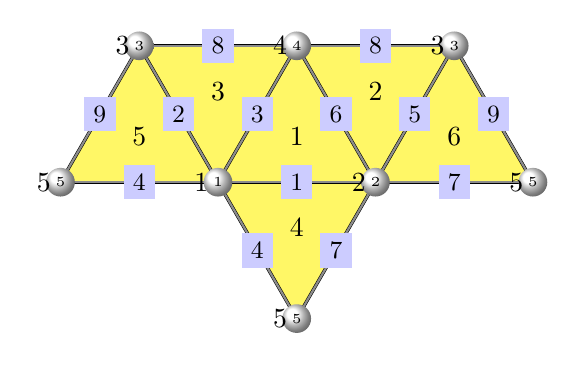
\begin{tikzpicture}[vertexBall, edgeDouble, faceStyle, scale=2]

% Define the coordinates of the vertices
\coordinate (V1_1) at (0., 0.);
\coordinate (V2_1) at (1., 0.);
\coordinate (V3_1) at (-0.5, 0.8660254037844384);
\coordinate (V3_2) at (1.5, 0.8660254037844388);
\coordinate (V4_1) at (0.4999999999999999, 0.8660254037844386);
\coordinate (V5_1) at (0.5000000000000001, -0.8660254037844386);
\coordinate (V5_2) at (-0.9999999999999996, 0.);
\coordinate (V5_3) at (2., 0.);


% Fill in the faces
\fill[face]  (V2_1) -- (V4_1) -- (V1_1) -- cycle;
\node[faceLabel] at (barycentric cs:V2_1=1,V4_1=1,V1_1=1) {$1$};
\fill[face]  (V2_1) -- (V3_2) -- (V4_1) -- cycle;
\node[faceLabel] at (barycentric cs:V2_1=1,V3_2=1,V4_1=1) {$2$};
\fill[face]  (V4_1) -- (V3_1) -- (V1_1) -- cycle;
\node[faceLabel] at (barycentric cs:V4_1=1,V3_1=1,V1_1=1) {$3$};
\fill[face]  (V1_1) -- (V5_1) -- (V2_1) -- cycle;
\node[faceLabel] at (barycentric cs:V1_1=1,V5_1=1,V2_1=1) {$4$};
\fill[face]  (V3_1) -- (V5_2) -- (V1_1) -- cycle;
\node[faceLabel] at (barycentric cs:V3_1=1,V5_2=1,V1_1=1) {$5$};
\fill[face]  (V2_1) -- (V5_3) -- (V3_2) -- cycle;
\node[faceLabel] at (barycentric cs:V2_1=1,V5_3=1,V3_2=1) {$6$};


% Draw the edges
\draw[edge] (V2_1) -- node[edgeLabel] {$1$} (V1_1);
\draw[edge] (V1_1) -- node[edgeLabel] {$2$} (V3_1);
\draw[edge] (V1_1) -- node[edgeLabel] {$3$} (V4_1);
\draw[edge] (V5_1) -- node[edgeLabel] {$4$} (V1_1);
\draw[edge] (V1_1) -- node[edgeLabel] {$4$} (V5_2);
\draw[edge] (V3_2) -- node[edgeLabel] {$5$} (V2_1);
\draw[edge] (V4_1) -- node[edgeLabel] {$6$} (V2_1);
\draw[edge] (V2_1) -- node[edgeLabel] {$7$} (V5_1);
\draw[edge] (V5_3) -- node[edgeLabel] {$7$} (V2_1);
\draw[edge] (V3_1) -- node[edgeLabel] {$8$} (V4_1);
\draw[edge] (V4_1) -- node[edgeLabel] {$8$} (V3_2);
\draw[edge] (V5_2) -- node[edgeLabel] {$9$} (V3_1);
\draw[edge] (V3_2) -- node[edgeLabel] {$9$} (V5_3);


% Draw the vertices
\vertexLabelR{V1_1}{left}{$1$}
\vertexLabelR{V2_1}{left}{$2$}
\vertexLabelR{V3_1}{left}{$3$}
\vertexLabelR{V3_2}{left}{$3$}
\vertexLabelR{V4_1}{left}{$4$}
\vertexLabelR{V5_1}{left}{$5$}
\vertexLabelR{V5_2}{left}{$5$}
\vertexLabelR{V5_3}{left}{$5$}

\end{tikzpicture}

\end{center}
 

 How do we find all children of t2? We could simply replace every possible face
by a tetrahedron and gather the constructed spheres up to isomorphism. But we
want to keep the number of tetrahedral extensions thus the expenses to a
minimum. Therefore we will use the automorphism group on the faces of our
spheres to determine the minimum number of faces and also the faces which have
to be replaced to obtain all children of t2. 

 
\begin{Verbatim}[commandchars=!@|,fontsize=\small,frame=single,label=Example]
  !gapprompt@gap>| !gapinput@a2:=AutomorphismGroupOnFaces(t2);|
  Group([ (1,2)(4,5), (2,3)(5,6), (1,4)(2,5)(3,6) ])
  !gapprompt@gap>| !gapinput@Orbits(a2);|
  [ [ 1, 2, 4, 3, 5, 6 ] ]
  !gapprompt@gap>| !gapinput@T3:=Sydi(T2,Te(3,4,5,6));|
  [ [ 1, 2, 3 ], [ 1, 2, 4 ], [ 1, 3, 4 ], [ 2, 3, 5 ], [ 2, 4, 5 ], 
   [ 3, 4, 6 ], [ 3, 5, 6 ], [ 4, 5, 6 ] ]
\end{Verbatim}
 

 So there is exactly one multi-tetrahedral sphere with 8 faces. 
\begin{center}
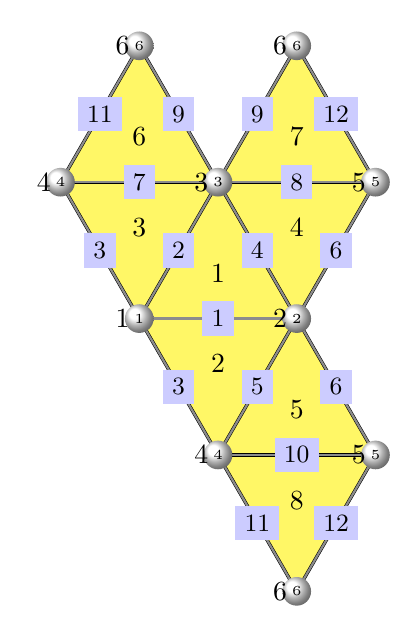
\begin{tikzpicture}[vertexBall, edgeDouble, faceStyle, scale=2]

% Define the coordinates of the vertices
\coordinate (V1_1) at (0, 0);
\coordinate (V2_1) at (1, 0);
\coordinate (V3_1) at (0.5, 0.8660254037844386);
\coordinate (V4_1) at (0.5, -0.8660254037844386);
\coordinate (V4_2) at (-0.4999999999999999, 0.8660254037844386);
\coordinate (V5_1) at (1.5, -0.8660254037844385);
\coordinate (V5_2) at (1.5, 0.8660254037844386);
\coordinate (V6_1) at (0, 1.732050807568877);
\coordinate (V6_2) at (0.9999999999999999, 1.732050807568877);
\coordinate (V6_3) at (1, -1.732050807568877);


% Fill in the faces
\fill[face]  (V2_1) -- (V3_1) -- (V1_1) -- cycle;
\node[faceLabel] at (barycentric cs:V2_1=1,V3_1=1,V1_1=1) {$1$};
\fill[face]  (V1_1) -- (V4_1) -- (V2_1) -- cycle;
\node[faceLabel] at (barycentric cs:V1_1=1,V4_1=1,V2_1=1) {$2$};
\fill[face]  (V3_1) -- (V4_2) -- (V1_1) -- cycle;
\node[faceLabel] at (barycentric cs:V3_1=1,V4_2=1,V1_1=1) {$3$};
\fill[face]  (V2_1) -- (V5_2) -- (V3_1) -- cycle;
\node[faceLabel] at (barycentric cs:V2_1=1,V5_2=1,V3_1=1) {$4$};
\fill[face]  (V4_1) -- (V5_1) -- (V2_1) -- cycle;
\node[faceLabel] at (barycentric cs:V4_1=1,V5_1=1,V2_1=1) {$5$};
\fill[face]  (V3_1) -- (V6_1) -- (V4_2) -- cycle;
\node[faceLabel] at (barycentric cs:V3_1=1,V6_1=1,V4_2=1) {$6$};
\fill[face]  (V5_2) -- (V6_2) -- (V3_1) -- cycle;
\node[faceLabel] at (barycentric cs:V5_2=1,V6_2=1,V3_1=1) {$7$};
\fill[face]  (V4_1) -- (V6_3) -- (V5_1) -- cycle;
\node[faceLabel] at (barycentric cs:V4_1=1,V6_3=1,V5_1=1) {$8$};


% Draw the edges
\draw[edge] (V2_1) -- node[edgeLabel] {$1$} (V1_1);
\draw[edge] (V1_1) -- node[edgeLabel] {$2$} (V3_1);
\draw[edge] (V4_1) -- node[edgeLabel] {$3$} (V1_1);
\draw[edge] (V1_1) -- node[edgeLabel] {$3$} (V4_2);
\draw[edge] (V3_1) -- node[edgeLabel] {$4$} (V2_1);
\draw[edge] (V2_1) -- node[edgeLabel] {$5$} (V4_1);
\draw[edge] (V2_1) -- node[edgeLabel] {$6$} (V5_1);
\draw[edge] (V5_2) -- node[edgeLabel] {$6$} (V2_1);
\draw[edge] (V4_2) -- node[edgeLabel] {$7$} (V3_1);
\draw[edge] (V3_1) -- node[edgeLabel] {$8$} (V5_2);
\draw[edge] (V6_1) -- node[edgeLabel] {$9$} (V3_1);
\draw[edge] (V3_1) -- node[edgeLabel] {$9$} (V6_2);
\draw[edge] (V5_1) -- node[edgeLabel] {$10$} (V4_1);
\draw[edge] (V4_2) -- node[edgeLabel] {$11$} (V6_1);
\draw[edge] (V6_3) -- node[edgeLabel] {$11$} (V4_1);
\draw[edge] (V6_2) -- node[edgeLabel] {$12$} (V5_2);
\draw[edge] (V5_1) -- node[edgeLabel] {$12$} (V6_3);


% Draw the vertices
\vertexLabelR{V1_1}{left}{$1$}
\vertexLabelR{V2_1}{left}{$2$}
\vertexLabelR{V3_1}{left}{$3$}
\vertexLabelR{V4_1}{left}{$4$}
\vertexLabelR{V4_2}{left}{$4$}
\vertexLabelR{V5_1}{left}{$5$}
\vertexLabelR{V5_2}{left}{$5$}
\vertexLabelR{V6_1}{left}{$6$}
\vertexLabelR{V6_2}{left}{$6$}
\vertexLabelR{V6_3}{left}{$6$}

\end{tikzpicture}

\end{center}
 Note, we can find the automorphism group of a simplicial surface with n faces
with the help of the symmetric group of degree n. It is easy to see that the
symmetric group acts on the set M, whereby an element A of M has a cardinality
of n. The elements of A are subsets of the set of vertices of our surface
containing exactly three vertices. Then the automorphism group on faces can be
identified as the stabilizer of the set of vertices in faces of our
multi-tetrahedral sphere under the described group action. 

 
\begin{Verbatim}[commandchars=!@|,fontsize=\small,frame=single,label=Example]
  !gapprompt@gap>| !gapinput@A3:=Stabilizer(SymmetricGroup(6),T3,OnSetsSets);|
  Group([ (3,4), (1,6)(2,5) ])
  !gapprompt@gap>| !gapinput@Orbits(A3,T3,OnSets);|
  [ [ [ 1, 2, 3 ], [ 1, 2, 4 ], [ 3, 5, 6 ], [ 4, 5, 6 ] ], 
   [ [ 1, 3, 4 ], [ 3, 4, 6 ] ], [ [ 2, 3, 5 ], [ 2, 4, 5 ] ] ]
\end{Verbatim}
 

 So there are exactly three multi-tetrahedral spheres with 10 faces which at
the same time are all children of the same multi-tetrehedral sphere. They are
represented by the following set of faces represented by their vertices in
faces. 

 
\begin{Verbatim}[commandchars=!@|,fontsize=\small,frame=single,label=Example]
  !gapprompt@gap>| !gapinput@O3:=last;|
  [ [ [ 1, 2, 3 ], [ 1, 2, 4 ], [ 3, 5, 6 ], [ 4, 5, 6 ] ], 
   [ [ 1, 3, 4 ], [ 3, 4, 6 ] ], [ [ 2, 3, 5 ], [ 2, 4, 5 ] ] ]
  !gapprompt@gap>| !gapinput@T4x1:=Sydi(T3,Te(4,5,6,7));|
  [ [ 1, 2, 3 ], [ 1, 2, 4 ], [ 1, 3, 4 ], [ 2, 3, 5 ], [ 2, 4, 5 ], 
   [ 3, 4, 6 ], [ 3, 5, 6 ], [ 4, 5, 7 ], [ 4, 6, 7 ], [ 5, 6, 7 ] ]
  !gapprompt@gap>| !gapinput@T4x2:=Sydi(T3,Te(3,4,6,7));|
  [ [ 1, 2, 3 ], [ 1, 2, 4 ], [ 1, 3, 4 ], [ 2, 3, 5 ], [ 2, 4, 5 ], 
   [ 3, 4, 7 ], [ 3, 5, 6 ], [ 3, 6, 7 ], [ 4, 5, 6 ], [ 4, 6, 7 ] ]
  !gapprompt@gap>| !gapinput@T4x3:=Sydi(T3,Te(2,4,5,7));|
  [ [ 1, 2, 3 ], [ 1, 2, 4 ], [ 1, 3, 4 ], [ 2, 3, 5 ], [ 2, 4, 7 ], 
   [ 2, 5, 7 ], [ 3, 4, 6 ], [ 3, 5, 6 ], [ 4, 5, 6 ], [ 4, 5, 7 ] ]
\end{Verbatim}
 

 Comparing their vertex counters shows that they are indeed not isomorpic. 

 
\begin{Verbatim}[commandchars=!@|,fontsize=\small,frame=single,label=Example]
  !gapprompt@gap>| !gapinput@SimplicialSurfaceByVerticesInFaces(T4x1); VertexCounter(last);|
  simplicial surface (7 vertices, 15 edges, and 10 faces)
  [ [ 3, 2 ], [ 4, 2 ], [ 5, 2 ], [ 6, 1 ] ]
  !gapprompt@gap>| !gapinput@SimplicialSurfaceByVerticesInFaces(T4x2); VertexCounter(last);|
  simplicial surface (7 vertices, 15 edges, and 10 faces)
  [ [ 3, 2 ], [ 4, 3 ], [ 6, 2 ] ]
  !gapprompt@gap>| !gapinput@SimplicialSurfaceByVerticesInFaces(T4x3); VertexCounter(last);|
  simplicial surface (7 vertices, 15 edges, and 10 faces)
  [ [ 3, 3 ], [ 5, 3 ], [ 6, 1 ] ]
\end{Verbatim}
 

 Computing the children of t4x1: 

 
\begin{Verbatim}[commandchars=!@|,fontsize=\small,frame=single,label=Example]
  !gapprompt@gap>| !gapinput@A4x1:=Stabilizer(SymmetricGroup(7),T4x1,OnSetsSets);|
  Group([ (1,7)(2,6)(3,5) ])
  !gapprompt@gap>| !gapinput@O4x1:=Orbits(A4x1,T4x1,OnSets);|
  [ [ [ 1, 2, 3 ], [ 5, 6, 7 ] ], [ [ 1, 2, 4 ], [ 4, 6, 7 ] ], 
   [ [ 1, 3, 4 ], [ 4, 5, 7 ] ], [ [ 2, 3, 5 ], [ 3, 5, 6 ] ], 
   [ [ 2, 4, 5 ], [ 3, 4, 6 ] ] ]
  !gapprompt@gap>| !gapinput@T5x1:=Sydi(T4x1,Te(5,6,7,8));|
  [ [ 1, 2, 3 ], [ 1, 2, 4 ], [ 1, 3, 4 ], [ 2, 3, 5 ], [ 2, 4, 5 ], 
   [ 3, 4, 6 ], [ 3, 5, 6 ], [ 4, 5, 7 ], [ 4, 6, 7 ], [ 5, 6, 8 ], 
   [ 5, 7, 8 ], [ 6, 7, 8 ] ]
  !gapprompt@gap>| !gapinput@T5x2:=Sydi(T4x1,Te(4,6,7,8));|
  [ [ 1, 2, 3 ], [ 1, 2, 4 ], [ 1, 3, 4 ], [ 2, 3, 5 ], [ 2, 4, 5 ], 
   [ 3, 4, 6 ], [ 3, 5, 6 ], [ 4, 5, 7 ], [ 4, 6, 8 ], [ 4, 7, 8 ], 
   [ 5, 6, 7 ], [ 6, 7, 8 ] ]
  !gapprompt@gap>| !gapinput@T5x3:=Sydi(T4x1,Te(4,5,7,8));|
  [ [ 1, 2, 3 ], [ 1, 2, 4 ], [ 1, 3, 4 ], [ 2, 3, 5 ], [ 2, 4, 5 ], 
   [ 3, 4, 6 ], [ 3, 5, 6 ], [ 4, 5, 8 ], [ 4, 6, 7 ], [ 4, 7, 8 ], 
   [ 5, 6, 7 ], [ 5, 7, 8 ] ]
  !gapprompt@gap>| !gapinput@T5x4:=Sydi(T4x1,Te(3,5,6,8));|
  [ [ 1, 2, 3 ], [ 1, 2, 4 ], [ 1, 3, 4 ], [ 2, 3, 5 ], [ 2, 4, 5 ], 
   [ 3, 4, 6 ], [ 3, 5, 8 ], [ 3, 6, 8 ], [ 4, 5, 7 ], [ 4, 6, 7 ], 
   [ 5, 6, 7 ], [ 5, 6, 8 ] ]
  !gapprompt@gap>| !gapinput@T5x5:=Sydi(T4x1,Te(3,4,6,8));|
  [ [ 1, 2, 3 ], [ 1, 2, 4 ], [ 1, 3, 4 ], [ 2, 3, 5 ], [ 2, 4, 5 ], 
   [ 3, 4, 8 ], [ 3, 5, 6 ], [ 3, 6, 8 ], [ 4, 5, 7 ], [ 4, 6, 7 ], 
   [ 4, 6, 8 ], [ 5, 6, 7 ] ]
\end{Verbatim}
 

 Hence we have 5 non isomorphic descendents of t4x1. 

 Computing their vertex counter: 

 
\begin{Verbatim}[commandchars=!@|,fontsize=\small,frame=single,label=Example]
  !gapprompt@gap>| !gapinput@SimplicialSurfaceByVerticesInFaces(T5x1); VertexCounter(last);|
  simplicial surface (8 vertices, 18 edges, and 12 faces)
  [ [ 3, 2 ], [ 4, 2 ], [ 5, 2 ], [ 6, 2 ] ]
  !gapprompt@gap>| !gapinput@SimplicialSurfaceByVerticesInFaces(T5x2); VertexCounter(last);|
  simplicial surface (8 vertices, 18 edges, and 12 faces)
  [ [ 3, 2 ], [ 4, 2 ], [ 5, 3 ], [ 7, 1 ] ]
  !gapprompt@gap>| !gapinput@SimplicialSurfaceByVerticesInFaces(T5x3); VertexCounter(last);|
  simplicial surface (8 vertices, 18 edges, and 12 faces)
  [ [ 3, 2 ], [ 4, 3 ], [ 5, 1 ], [ 6, 1 ], [ 7, 1 ] ]
  !gapprompt@gap>| !gapinput@SimplicialSurfaceByVerticesInFaces(T5x4); VertexCounter(last);|
  simplicial surface (8 vertices, 18 edges, and 12 faces)
  [ [ 3, 3 ], [ 4, 1 ], [ 5, 1 ], [ 6, 3 ] ]
  !gapprompt@gap>| !gapinput@SimplicialSurfaceByVerticesInFaces(T5x5); VertexCounter(last);|
  simplicial surface (8 vertices, 18 edges, and 12 faces)
  [ [ 3, 3 ], [ 4, 1 ], [ 5, 2 ], [ 6, 1 ], [ 7, 1 ] ]
\end{Verbatim}
 

 Note, non isomorphic multi-tetrahedral spheres can still have isomorphic
children. But the vertex counter indicates whether two spheres are non
isomorphic. This is the case, if their vertex counters do differ. If they have
the same vertex counters we have to check whether there exists an isomorphism
mapping one to the other. 

 Compute the children of t4x2: 
\begin{Verbatim}[commandchars=!@|,fontsize=\small,frame=single,label=Example]
  !gapprompt@gap>| !gapinput@A4x2:=Stabilizer(SymmetricGroup(7),T4x2,OnSetsSets);|
  Group([ (3,4), (1,7)(2,6) ])
  !gapprompt@gap>| !gapinput@O4x2:=Orbits(A4x2,T4x2,OnSets);|
  [ [ [ 1, 2, 3 ], [ 1, 2, 4 ], [ 3, 6, 7 ], [ 4, 6, 7 ] ], 
   [ [ 1, 3, 4 ], [ 3, 4, 7 ] ], 
   [ [ 2, 3, 5 ], [ 2, 4, 5 ], [ 3, 5, 6 ], [ 4, 5, 6 ] ] ]
  !gapprompt@gap>| !gapinput@T5x6:=Sydi(T4x2,Te(4,6,7,8));|
  [ [ 1, 2, 3 ], [ 1, 2, 4 ], [ 1, 3, 4 ], [ 2, 3, 5 ], [ 2, 4, 5 ], 
   [ 3, 4, 7 ], [ 3, 5, 6 ], [ 3, 6, 7 ], [ 4, 5, 6 ], [ 4, 6, 8 ], 
   [ 4, 7, 8 ], [ 6, 7, 8 ] ]
  !gapprompt@gap>| !gapinput@SimplicialSurfaceByVerticesInFaces(T5x6); VertexCounter(last);|
  simplicial surface (8 vertices, 18 edges, and 12 faces)
  [ [ 3, 2 ], [ 4, 3 ], [ 5, 1 ], [ 6, 1 ], [ 7, 1 ] ]
  !gapprompt@gap>| !gapinput@T5x6 in Orbit(SymmetricGroup(8),T5x3,OnSetsSets);|
  true
\end{Verbatim}
 

 
\begin{center}
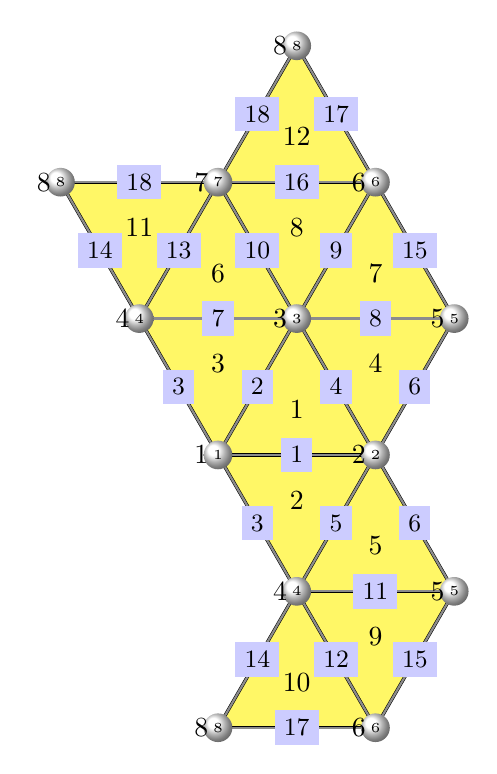
\begin{tikzpicture}[vertexBall, edgeDouble, faceStyle, scale=2]

% Define the coordinates of the vertices
\coordinate (V1_1) at (0, 0);
\coordinate (V2_1) at (1, 0);
\coordinate (V3_1) at (0.5, 0.8660254037844386);
\coordinate (V4_1) at (0.5, -0.8660254037844386);
\coordinate (V4_2) at (-0.4999999999999999, 0.8660254037844386);
\coordinate (V5_1) at (1.5, -0.8660254037844386);
\coordinate (V5_2) at (1.5, 0.8660254037844386);
\coordinate (V6_1) at (0.9999999999999999, 1.732050807568877);
\coordinate (V6_2) at (1, -1.732050807568877);
\coordinate (V7_1) at (0, 1.732050807568877);
\coordinate (V8_1) at (0, -1.732050807568877);
\coordinate (V8_2) at (-0.9999999999999999, 1.732050807568877);
\coordinate (V8_3) at (0.4999999999999999, 2.598076211353316);


% Fill in the faces
\fill[face]  (V2_1) -- (V3_1) -- (V1_1) -- cycle;
\node[faceLabel] at (barycentric cs:V2_1=1,V3_1=1,V1_1=1) {$1$};
\fill[face]  (V1_1) -- (V4_1) -- (V2_1) -- cycle;
\node[faceLabel] at (barycentric cs:V1_1=1,V4_1=1,V2_1=1) {$2$};
\fill[face]  (V3_1) -- (V4_2) -- (V1_1) -- cycle;
\node[faceLabel] at (barycentric cs:V3_1=1,V4_2=1,V1_1=1) {$3$};
\fill[face]  (V2_1) -- (V5_2) -- (V3_1) -- cycle;
\node[faceLabel] at (barycentric cs:V2_1=1,V5_2=1,V3_1=1) {$4$};
\fill[face]  (V4_1) -- (V5_1) -- (V2_1) -- cycle;
\node[faceLabel] at (barycentric cs:V4_1=1,V5_1=1,V2_1=1) {$5$};
\fill[face]  (V3_1) -- (V7_1) -- (V4_2) -- cycle;
\node[faceLabel] at (barycentric cs:V3_1=1,V7_1=1,V4_2=1) {$6$};
\fill[face]  (V5_2) -- (V6_1) -- (V3_1) -- cycle;
\node[faceLabel] at (barycentric cs:V5_2=1,V6_1=1,V3_1=1) {$7$};
\fill[face]  (V6_1) -- (V7_1) -- (V3_1) -- cycle;
\node[faceLabel] at (barycentric cs:V6_1=1,V7_1=1,V3_1=1) {$8$};
\fill[face]  (V4_1) -- (V6_2) -- (V5_1) -- cycle;
\node[faceLabel] at (barycentric cs:V4_1=1,V6_2=1,V5_1=1) {$9$};
\fill[face]  (V4_1) -- (V8_1) -- (V6_2) -- cycle;
\node[faceLabel] at (barycentric cs:V4_1=1,V8_1=1,V6_2=1) {$10$};
\fill[face]  (V7_1) -- (V8_2) -- (V4_2) -- cycle;
\node[faceLabel] at (barycentric cs:V7_1=1,V8_2=1,V4_2=1) {$11$};
\fill[face]  (V6_1) -- (V8_3) -- (V7_1) -- cycle;
\node[faceLabel] at (barycentric cs:V6_1=1,V8_3=1,V7_1=1) {$12$};


% Draw the edges
\draw[edge] (V2_1) -- node[edgeLabel] {$1$} (V1_1);
\draw[edge] (V1_1) -- node[edgeLabel] {$2$} (V3_1);
\draw[edge] (V4_1) -- node[edgeLabel] {$3$} (V1_1);
\draw[edge] (V1_1) -- node[edgeLabel] {$3$} (V4_2);
\draw[edge] (V3_1) -- node[edgeLabel] {$4$} (V2_1);
\draw[edge] (V2_1) -- node[edgeLabel] {$5$} (V4_1);
\draw[edge] (V2_1) -- node[edgeLabel] {$6$} (V5_1);
\draw[edge] (V5_2) -- node[edgeLabel] {$6$} (V2_1);
\draw[edge] (V4_2) -- node[edgeLabel] {$7$} (V3_1);
\draw[edge] (V3_1) -- node[edgeLabel] {$8$} (V5_2);
\draw[edge] (V3_1) -- node[edgeLabel] {$9$} (V6_1);
\draw[edge] (V7_1) -- node[edgeLabel] {$10$} (V3_1);
\draw[edge] (V5_1) -- node[edgeLabel] {$11$} (V4_1);
\draw[edge] (V6_2) -- node[edgeLabel] {$12$} (V4_1);
\draw[edge] (V4_2) -- node[edgeLabel] {$13$} (V7_1);
\draw[edge] (V8_1) -- node[edgeLabel] {$14$} (V4_1);
\draw[edge] (V4_2) -- node[edgeLabel] {$14$} (V8_2);
\draw[edge] (V6_1) -- node[edgeLabel] {$15$} (V5_2);
\draw[edge] (V5_1) -- node[edgeLabel] {$15$} (V6_2);
\draw[edge] (V7_1) -- node[edgeLabel] {$16$} (V6_1);
\draw[edge] (V6_2) -- node[edgeLabel] {$17$} (V8_1);
\draw[edge] (V8_3) -- node[edgeLabel] {$17$} (V6_1);
\draw[edge] (V8_2) -- node[edgeLabel] {$18$} (V7_1);
\draw[edge] (V7_1) -- node[edgeLabel] {$18$} (V8_3);


% Draw the vertices
\vertexLabelR{V1_1}{left}{$1$}
\vertexLabelR{V2_1}{left}{$2$}
\vertexLabelR{V3_1}{left}{$3$}
\vertexLabelR{V4_1}{left}{$4$}
\vertexLabelR{V4_2}{left}{$4$}
\vertexLabelR{V5_1}{left}{$5$}
\vertexLabelR{V5_2}{left}{$5$}
\vertexLabelR{V6_1}{left}{$6$}
\vertexLabelR{V6_2}{left}{$6$}
\vertexLabelR{V7_1}{left}{$7$}
\vertexLabelR{V8_1}{left}{$8$}
\vertexLabelR{V8_2}{left}{$8$}
\vertexLabelR{V8_3}{left}{$8$}

\end{tikzpicture}

\end{center}
 

 So the sphere represented by T5x6 is a child of t4x1 and t4x2. Alternatively
the isomorphism check can be done by constructing the spheres and using \texttt{IsIsomorphic()} 

 Compute the remaining children of t4x2: 

 
\begin{Verbatim}[commandchars=!@|,fontsize=\small,frame=single,label=Example]
  !gapprompt@gap>| !gapinput@T5x6:=Sydi(T4x2,Te(3,4,7,8));|
  [ [ 1, 2, 3 ], [ 1, 2, 4 ], [ 1, 3, 4 ], [ 2, 3, 5 ], [ 2, 4, 5 ], 
    [ 3, 4, 8 ], [ 3, 5, 6 ], [ 3, 6, 7 ], [ 3, 7, 8 ], [ 4, 5, 6 ], 
    [ 4, 6, 7 ], [ 4, 7, 8 ] ]
  !gapprompt@gap>| !gapinput@SimplicialSurfaceByVerticesInFaces(T5x6); VertexCounter(last);|
  simplicial surface (8 vertices, 18 edges, and 12 faces)
  [ [ 3, 2 ], [ 4, 4 ], [ 7, 2 ] ]
  !gapprompt@gap>| !gapinput@T5x7:=Sydi(T4x2,Te(4,5,6,8));|
  [ [ 1, 2, 3 ], [ 1, 2, 4 ], [ 1, 3, 4 ], [ 2, 3, 5 ], [ 2, 4, 5 ], 
    [ 3, 4, 7 ], [ 3, 5, 6 ], [ 3, 6, 7 ], [ 4, 5, 8 ], [ 4, 6, 7 ], 
    [ 4, 6, 8 ], [ 5, 6, 8 ] ]
  !gapprompt@gap>| !gapinput@SimplicialSurfaceByVerticesInFaces(T5x6); VertexCounter(last);|
  simplicial surface (8 vertices, 18 edges, and 12 faces)
  [ [ 3, 2 ], [ 4, 4 ], [ 7, 2 ] ]
  !gapprompt@gap>| !gapinput@SimplicialSurfaceByVerticesInFaces(T5x7); VertexCounter(last);|
  simplicial surface (8 vertices, 18 edges, and 12 faces)
  [ [ 3, 3 ], [ 4, 1 ], [ 5, 2 ], [ 6, 1 ], [ 7, 1 ] ]
  !gapprompt@gap>| !gapinput@SimplicialSurfaceByVerticesInFaces(T5x5); VertexCounter(last);|
  simplicial surface (8 vertices, 18 edges, and 12 faces)
  [ [ 3, 3 ], [ 4, 1 ], [ 5, 2 ], [ 6, 1 ], [ 7, 1 ] ]
  !gapprompt@gap>| !gapinput@T5x7 in Orbit(SymmetricGroup(8),T5x5,OnSetsSets);|
  true
\end{Verbatim}
 

 So computing the children of t4x2 gives rise to three non isomorphic multi-
tetrahedral spheres of which two are also children of t4x1. 

 Constructing the children of t4x3: 

 
\begin{Verbatim}[commandchars=!@|,fontsize=\small,frame=single,label=Example]
  !gapprompt@gap>| !gapinput@A4x3:=Stabilizer(SymmetricGroup(7),T4x3,OnSetsSets);|
  Group([ (2,3)(6,7), (1,7)(3,5) ])
  !gapprompt@gap>| !gapinput@O4x3:=Orbits(A4x3,T4x3,OnSets);|
  [ [ [ 1, 2, 3 ], [ 3, 5, 6 ], [ 2, 5, 7 ] ], 
    [ [ 1, 2, 4 ], [ 3, 4, 6 ], [ 4, 5, 7 ], [ 1, 3, 4 ], [ 2, 4, 7 ], 
        [ 4, 5, 6 ] ], [ [ 2, 3, 5 ] ] ]
\end{Verbatim}
 

 Hence the multitetradral-sphere T4x3 has exactly three children. 

 
\begin{Verbatim}[commandchars=!@|,fontsize=\small,frame=single,label=Example]
  !gapprompt@gap>| !gapinput@T5x7:=Sydi(T4x3,Te(2,5,7,8));|
  [ [ 1, 2, 3 ], [ 1, 2, 4 ], [ 1, 3, 4 ], [ 2, 3, 5 ], [ 2, 4, 7 ], 
    [ 2, 5, 8 ], [ 2, 7, 8 ], [ 3, 4, 6 ], [ 3, 5, 6 ], [ 4, 5, 6 ], 
    [ 4, 5, 7 ], [ 5, 7, 8 ] ]
  !gapprompt@gap>| !gapinput@SimplicialSurfaceByVerticesInFaces(T5x7); VertexCounter(last);|
  simplicial surface (8 vertices, 18 edges, and 12 faces)
  [ [ 3, 3 ], [ 4, 1 ], [ 5, 1 ], [ 6, 3 ] ]
  !gapprompt@gap>| !gapinput@T5x7 in Orbit(SymmetricGroup(8),T5x4,OnSetsSets);|
  true
  !gapprompt@gap>| !gapinput@T5x7:=Sydi(T4x3,Te(4,5,6,8));|
  [ [ 1, 2, 3 ], [ 1, 2, 4 ], [ 1, 3, 4 ], [ 2, 3, 5 ], [ 2, 4, 7 ], 
    [ 2, 5, 7 ], [ 3, 4, 6 ], [ 3, 5, 6 ], [ 4, 5, 7 ], [ 4, 5, 8 ], 
    [ 4, 6, 8 ], [ 5, 6, 8 ] ]
  !gapprompt@gap>| !gapinput@SimplicialSurfaceByVerticesInFaces(T5x7); VertexCounter(last);|
  simplicial surface (8 vertices, 18 edges, and 12 faces)
  [ [ 3, 3 ], [ 4, 1 ], [ 5, 2 ], [ 6, 1 ], [ 7, 1 ] ]
  !gapprompt@gap>| !gapinput@T5x7 in Orbit(SymmetricGroup(8),T5x5,OnSetsSets);|
  true
  !gapprompt@gap>| !gapinput@T5x7:=Sydi(T4x3,Te(2,3,5,8));|
  [ [ 1, 2, 3 ], [ 1, 2, 4 ], [ 1, 3, 4 ], [ 2, 3, 8 ], [ 2, 4, 7 ], 
    [ 2, 5, 7 ], [ 2, 5, 8 ], [ 3, 4, 6 ], [ 3, 5, 6 ], [ 3, 5, 8 ], 
    [ 4, 5, 6 ], [ 4, 5, 7 ] ]
  !gapprompt@gap>| !gapinput@SimplicialSurfaceByVerticesInFaces(T5x7); VertexCounter(last);|
  simplicial surface (8 vertices, 18 edges, and 12 faces)
  [ [ 3, 4 ], [ 6, 4 ] ]
  !gapprompt@gap>| !gapinput@VC5:=List([T5x1,T5x2,T5x3,T5x4,T5x5,T5x6,T5x7],r- |
  >VertexCounter(SimplicialSurfaceByVerticesInFaces(r)));
  [ [ [ 3, 2 ], [ 4, 2 ], [ 5, 2 ], [ 6, 2 ] ], 
    [ [ 3, 2 ], [ 4, 2 ], [ 5, 3 ], [ 7, 1 ] ], 
    [ [ 3, 2 ], [ 4, 3 ], [ 5, 1 ], [ 6, 1 ], [ 7, 1 ] ], 
    [ [ 3, 3 ], [ 4, 1 ], [ 5, 1 ], [ 6, 3 ] ], 
    [ [ 3, 3 ], [ 4, 1 ], [ 5, 2 ], [ 6, 1 ], [ 7, 1 ] ], 
    [ [ 3, 2 ], [ 4, 4 ], [ 7, 2 ] ], [ [ 3, 4 ], [ 6, 4 ] ] ]
\end{Verbatim}
 

 So out of the three children two are also children of t4x2. So in total there
are exactly seven multi-tetrahedral spheres with 12 faces up to isomorphism.
The last sphere with vertex counter \texttt{[[3,4],[6,4]]} is of greater interest to us. 

 
\begin{center}
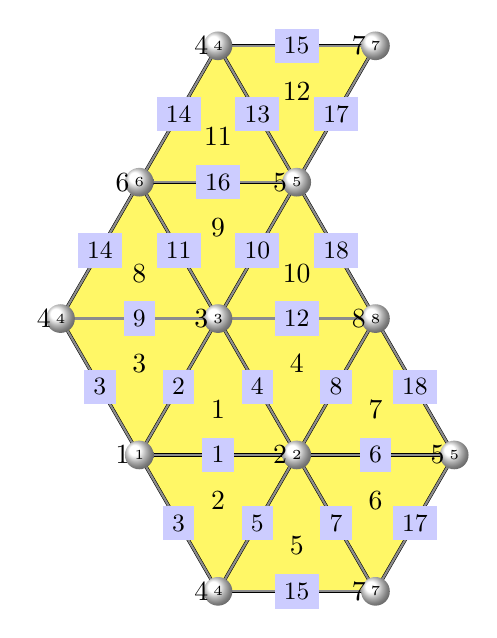
\begin{tikzpicture}[vertexBall, edgeDouble, faceStyle, scale=2]

% Define the coordinates of the vertices
\coordinate (V1_1) at (0, 0);
\coordinate (V2_1) at (1, 0);
\coordinate (V3_1) at (0.5, 0.8660254037844386);
\coordinate (V4_1) at (0.5, -0.8660254037844386);
\coordinate (V4_2) at (-0.4999999999999999, 0.8660254037844386);
\coordinate (V4_3) at (0.4999999999999999, 2.598076211353316);
\coordinate (V5_1) at (2, 0);
\coordinate (V5_2) at (0.9999999999999999, 1.732050807568877);
\coordinate (V6_1) at (0, 1.732050807568877);
\coordinate (V7_1) at (1.5, -0.8660254037844386);
\coordinate (V7_2) at (1.5, 2.598076211353316);
\coordinate (V8_1) at (1.5, 0.8660254037844386);


% Fill in the faces
\fill[face]  (V2_1) -- (V3_1) -- (V1_1) -- cycle;
\node[faceLabel] at (barycentric cs:V2_1=1,V3_1=1,V1_1=1) {$1$};
\fill[face]  (V1_1) -- (V4_1) -- (V2_1) -- cycle;
\node[faceLabel] at (barycentric cs:V1_1=1,V4_1=1,V2_1=1) {$2$};
\fill[face]  (V3_1) -- (V4_2) -- (V1_1) -- cycle;
\node[faceLabel] at (barycentric cs:V3_1=1,V4_2=1,V1_1=1) {$3$};
\fill[face]  (V2_1) -- (V8_1) -- (V3_1) -- cycle;
\node[faceLabel] at (barycentric cs:V2_1=1,V8_1=1,V3_1=1) {$4$};
\fill[face]  (V4_1) -- (V7_1) -- (V2_1) -- cycle;
\node[faceLabel] at (barycentric cs:V4_1=1,V7_1=1,V2_1=1) {$5$};
\fill[face]  (V7_1) -- (V5_1) -- (V2_1) -- cycle;
\node[faceLabel] at (barycentric cs:V7_1=1,V5_1=1,V2_1=1) {$6$};
\fill[face]  (V2_1) -- (V5_1) -- (V8_1) -- cycle;
\node[faceLabel] at (barycentric cs:V2_1=1,V5_1=1,V8_1=1) {$7$};
\fill[face]  (V3_1) -- (V6_1) -- (V4_2) -- cycle;
\node[faceLabel] at (barycentric cs:V3_1=1,V6_1=1,V4_2=1) {$8$};
\fill[face]  (V3_1) -- (V5_2) -- (V6_1) -- cycle;
\node[faceLabel] at (barycentric cs:V3_1=1,V5_2=1,V6_1=1) {$9$};
\fill[face]  (V8_1) -- (V5_2) -- (V3_1) -- cycle;
\node[faceLabel] at (barycentric cs:V8_1=1,V5_2=1,V3_1=1) {$10$};
\fill[face]  (V5_2) -- (V4_3) -- (V6_1) -- cycle;
\node[faceLabel] at (barycentric cs:V5_2=1,V4_3=1,V6_1=1) {$11$};
\fill[face]  (V5_2) -- (V7_2) -- (V4_3) -- cycle;
\node[faceLabel] at (barycentric cs:V5_2=1,V7_2=1,V4_3=1) {$12$};


% Draw the edges
\draw[edge] (V2_1) -- node[edgeLabel] {$1$} (V1_1);
\draw[edge] (V1_1) -- node[edgeLabel] {$2$} (V3_1);
\draw[edge] (V4_1) -- node[edgeLabel] {$3$} (V1_1);
\draw[edge] (V1_1) -- node[edgeLabel] {$3$} (V4_2);
\draw[edge] (V3_1) -- node[edgeLabel] {$4$} (V2_1);
\draw[edge] (V2_1) -- node[edgeLabel] {$5$} (V4_1);
\draw[edge] (V2_1) -- node[edgeLabel] {$6$} (V5_1);
\draw[edge] (V2_1) -- node[edgeLabel] {$7$} (V7_1);
\draw[edge] (V8_1) -- node[edgeLabel] {$8$} (V2_1);
\draw[edge] (V4_2) -- node[edgeLabel] {$9$} (V3_1);
\draw[edge] (V5_2) -- node[edgeLabel] {$10$} (V3_1);
\draw[edge] (V6_1) -- node[edgeLabel] {$11$} (V3_1);
\draw[edge] (V3_1) -- node[edgeLabel] {$12$} (V8_1);
\draw[edge] (V4_3) -- node[edgeLabel] {$13$} (V5_2);
\draw[edge] (V4_2) -- node[edgeLabel] {$14$} (V6_1);
\draw[edge] (V6_1) -- node[edgeLabel] {$14$} (V4_3);
\draw[edge] (V7_1) -- node[edgeLabel] {$15$} (V4_1);
\draw[edge] (V4_3) -- node[edgeLabel] {$15$} (V7_2);
\draw[edge] (V6_1) -- node[edgeLabel] {$16$} (V5_2);
\draw[edge] (V5_1) -- node[edgeLabel] {$17$} (V7_1);
\draw[edge] (V7_2) -- node[edgeLabel] {$17$} (V5_2);
\draw[edge] (V8_1) -- node[edgeLabel] {$18$} (V5_1);
\draw[edge] (V5_2) -- node[edgeLabel] {$18$} (V8_1);


% Draw the vertices
\vertexLabelR{V1_1}{left}{$1$}
\vertexLabelR{V2_1}{left}{$2$}
\vertexLabelR{V3_1}{left}{$3$}
\vertexLabelR{V4_1}{left}{$4$}
\vertexLabelR{V4_2}{left}{$4$}
\vertexLabelR{V4_3}{left}{$4$}
\vertexLabelR{V5_1}{left}{$5$}
\vertexLabelR{V5_2}{left}{$5$}
\vertexLabelR{V6_1}{left}{$6$}
\vertexLabelR{V7_1}{left}{$7$}
\vertexLabelR{V7_2}{left}{$7$}
\vertexLabelR{V8_1}{left}{$8$}

\end{tikzpicture}

\end{center}
 
\begin{Verbatim}[commandchars=!@|,fontsize=\small,frame=single,label=Example]
  !gapprompt@gap>| !gapinput@t5x7:=SimplicialSurfaceByVerticesInFaces(T5x7);|
  simplicial surface (8 vertices, 18 edges, and 12 faces)
  !gapprompt@gap>| !gapinput@FaceCounter(t5x7);|
  [ [ [ 3, 6, 6 ], 12 ] ]
\end{Verbatim}
 

 One could get the idea that this is a multi-tetrahedral sphere obtained from a
tetrahedron where every face is subdivided due to tetrahedral extension 

 
\begin{Verbatim}[commandchars=!@|,fontsize=\small,frame=single,label=Example]
  !gapprompt@gap>| !gapinput@Filtered(Vertices(t5x7),r->FaceDegreeOfVertex(t5x7,r)=3);|
  [ 1, 6, 7, 8 ]
  !gapprompt@gap>| !gapinput@List(last,i->NeighbourVerticesOfVertex(t5x7,i));|
  [ [ 2, 3, 4 ], [ 3, 4, 5 ], [ 2, 4, 5 ], [ 2, 3, 5 ] ]
  !gapprompt@gap>| !gapinput@Te(2,3,4,5);|
  [ [ 2, 3, 4 ], [ 2, 3, 5 ], [ 2, 4, 5 ], [ 3, 4, 5 ] ]
  !gapprompt@gap>| !gapinput@Set(last2)=last;|
  true 
\end{Verbatim}
 

 
\begin{center}
\input{tikzpictures/Image_Tetrahedron_4Extensions.tex}
\end{center}
 

 }

 }

 
\section{\textcolor{Chapter }{Isosceles coloured Surfaces}}\label{Section_IsoscelescolouredSurfaces}
\logpage{[ 3, 4, 0 ]}
\hyperdef{L}{X7F5AF9807BD3C3D6}{}
{
  

 $Problems:$ Analysing Isosceles coloured surfaces 

 $Theoretical$ $background$ 
\begin{itemize}
\item  isosceles coloured surfaces and boolean operations 
\end{itemize}
 

 $Frequently$ $used$ $commands$ 
\begin{itemize}
\item  AllIsoscelesColouredSurfaces() (\ref{AllIsoscelesColouredSurfaces}) 
\item  AllSimplicialSpheres() (\ref{AllSimplicialSpheres}) 
\item  EdgesOfFaces() (local version: EdgesOfFace()) (\ref{EdgesOfFaces}) 
\item  FaceDegreesOfVertices() (local version: FaceDegreeOfVertex) (\ref{FaceDegreesOfVertices}) 
\item  NeighbourVerticesOfVertex() (\ref{NeighbourVerticesOfVertex}), 
\item  SubcomplexByFaces() (\ref{SubcomplexByFaces}) 
\item  VertexCounter() (local version: DegreeOfVertex()) (\ref{VertexCounter}), 
\item  VerticesOfFaces() (local Version: VerticesOfFace()) (\ref{VerticesOfFaces}) 
\item  UmbrellaPathsOfVertices() (local version: UmbrellaPathOfVertex()) (\ref{UmbrellaPathsOfVertices}) 
\end{itemize}
 $ Mathematical$ $details:$ 

 Most of what has been said in the previous exercises applies for arbitrary
simplicial surfaces and simplicial surfaces of equiangular triangles. This
chapter deals with the combinatorial side of simplicial surfaces of congruent
isoscles triangules. More precisely we want to investigate those simplicial
surfaces whose isosceles triangules are not equiangular. 

 
\begin{center}
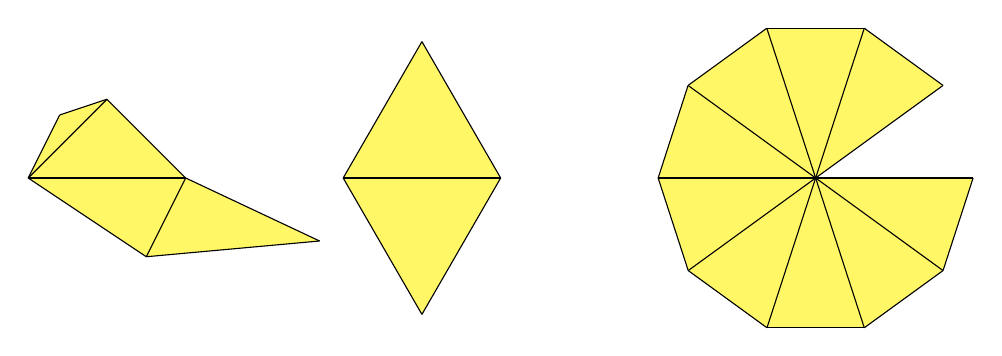
\begin{tikzpicture}[vertexBall, edgeDouble, faceStyle, scale=2, edgeStyle=nolabels,vertexStyle=nolabels]
\coordinate (V1) at (0.5, 0.8660254037844386);
\coordinate (V2) at (0, 0);
\coordinate (V3) at (1, 0);
\coordinate (V4) at (0.5, -0.8660254037844386);

\coordinate (V12) at (-1.5, 0.5);
\coordinate (V22) at (-1, 0);
\coordinate (V32) at (-2, 0);
\coordinate (V42) at (-1.25, -0.5);
\coordinate (V52) at (-1.8, 0.4);
\coordinate (V62) at (-0.15, -0.4);


\coordinate (V13) at ( 3.8090169943749475, 0.5877852522924731);
\coordinate (V23) at ( 3.3090169943749475, 0.9510565162951535 );
\coordinate (V33) at ( 2.69, 0.9510565162951536 );
\coordinate (V43) at ( 2.19, 0.5877852522924732 );
\coordinate (V53) at ( 2,0 );
\coordinate (V63) at ( 2.191, -0.587785252292473 );
\coordinate (V73) at ( 2.691, -0.9510565162951535 );
\coordinate (V83) at ( 3.3090169943749472, -0.9510565162951536 );
\coordinate (V93) at ( 3.8090169943749473, -0.5877852522924734 );
\coordinate (V103) at ( 4, 0);
\coordinate (z) at ( 3, 0);

\fill[face]  (V3) -- (V1) -- (V2) -- cycle;
\node[faceLabel] at (barycentric cs:V3=1,V1=1,V2=1) {};
\fill[face]  (V3) -- (V4) -- (V2) -- cycle;
\node[faceLabel] at (barycentric cs:V3=1,V4=1,V2=1) {};

\fill[face]  (V32) -- (V12) -- (V22) -- cycle;
\node[faceLabel] at (barycentric cs:V32=1,V12=1,V22=1) {};
\fill[face]  (V32) -- (V42) -- (V22) -- cycle;
\node[faceLabel] at (barycentric cs:V32=1,V12=1,V22=1) {};
\fill[face]  (V52) -- (V32) -- (V12) -- cycle;
\fill[face]  (V62) -- (V42) -- (V22) -- cycle;

\fill[face]  (z) -- (V13) -- (V23) -- cycle;
\fill[face]  (z) -- (V23) -- (V33) -- cycle;
\fill[face]  (z) -- (V33) -- (V43) -- cycle;
\fill[face]  (z) -- (V43) -- (V53) -- cycle;
\fill[face]  (z) -- (V53) -- (V63) -- cycle;
\fill[face]  (z) -- (V63) -- (V73) -- cycle;
\fill[face]  (z) -- (V73) -- (V83) -- cycle;
\fill[face]  (z) -- (V83) -- (V93) -- cycle;
\fill[face]  (z) -- (V93) -- (V103) -- cycle;
%\node[faceLabel] at (barycentric cs:V3=1,V1=1,V2=1) {};
%\node[faceLabel] at (barycentric cs:V32=1,V12=1,V22=1) {};
\draw[edge=black] (V1) -- (V2);
\draw[edge=black] (V1) -- (V3);
\draw[edge=black] (V3) -- (V2);
\draw[edge=black] (V4) -- (V2);
\draw[edge=black] (V3) -- (V4);

\draw[edge=black] (V62) -- (V42);
\draw[edge=black] (V62) -- (V22);
\draw[edge=black] (V12) -- (V22);
\draw[edge=black] (V12) -- (V32);
\draw[edge=black] (V32) -- (V22);
\draw[edge=black] (V42) -- (V22);
\draw[edge=black] (V32) -- (V42);
\draw[edge=black] (V12) -- (V52);
\draw[edge=black] (V32) -- (V52);
%\draw[edge=black] (V32) -- (V42);

 \foreach \x in {V13,V23,V33,V43,V53,V63,V73,V83,V93,V103}{
                    \draw[edge=black] (z) -- (\x);
                }

\draw[edge=black] (V13) -- (V23);
\draw[edge=black] (V23) -- (V33);
\draw[edge=black] (V33) -- (V43);
\draw[edge=black] (V43) -- (V53);
\draw[edge=black] (V53) -- (V63);
\draw[edge=black] (V63) -- (V73);
\draw[edge=black] (V73) -- (V83);
\draw[edge=black] (V83) -- (V93);
\draw[edge=black] (V93) -- (V103);



\end{tikzpicture}


\end{center}
 

 Therefore we define the base selection or simply base of a simplicial surface
as a subset of the edges underlying the condition that every face of the
surface is incident to exactly one edge of the base. We shall refer to an edge
as base edge if it is contained in the base and as a leg if it is not. This
gives rise to two types of vertices of a face. If a vertex of a face is
incident to the two legs of the face, then we call it apex vertex or simply
apex. So each face is incident to exactly one apex. 

 
\begin{center}
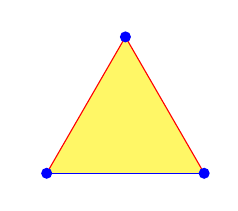
\begin{tikzpicture}[vertexBall, edgeDouble, faceStyle, scale=2, edgeStyle=nolabels,vertexStyle=nolabels]
\coordinate (V1_1) at (0.5, 0.8660254037844386);
\coordinate (V2_1) at (0, 0);
\coordinate (V3_1) at (1, 0);

\fill[face]  (V3_1) -- (V1_1) -- (V2_1) -- cycle;
\node[faceLabel] at (barycentric cs:V3_1=1,V1_1=1,V2_1=1) {};

\draw[edge=red] (V1_1) -- (V2_1);
\draw[edge=blue] (V2_1) -- (V3_1);
\draw[edge=red] (V1_1) -- (V3_1);

\vertexLabelR{V1_1}{left}{}
\vertexLabelR{V2_1}{left}{}
\vertexLabelR{V3_1}{left}{}
\end{tikzpicture}

\end{center}
 

 We handle simplical surfaces of isosceles triangles in the package by
introducing a colouring for edges and call the resulting structures isosceles
coloured simplicial surfaces. For example up to isomorphism there is exactly
one isosceles coloured surface resulting from the tetrahedron. 

 
\begin{Verbatim}[commandchars=!@|,fontsize=\small,frame=single,label=Example]
  !gapprompt@gap>| !gapinput@pr:=rec(edgeColourClassColours:=["red","blue"]);;|
  !gapprompt@gap>| !gapinput@AllIsoscelesColouredSurfaces(T);|
  [ isosceles coloured surface (4 vertices, 6 edges and 4 faces) ]
  !gapprompt@gap>| !gapinput@DrawSurfaceToTikz(last[1],"Image_IsoscelesColouredTetrahedron1.tex",pr);|
  Picture written in TikZ.
\end{Verbatim}
 

 
\begin{center}
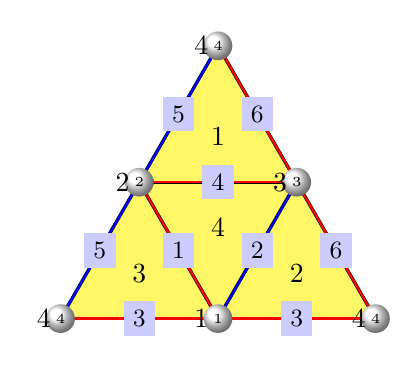
\begin{tikzpicture}[vertexBall, edgeDouble, faceStyle, scale=2]

% Define the coordinates of the vertices
\coordinate (V1_1) at (0.5, -0.8660254037844386);
\coordinate (V2_1) at (0, 0);
\coordinate (V3_1) at (1, 0);
\coordinate (V4_1) at (0.4999999999999999, 0.8660254037844386);
\coordinate (V4_2) at (-0.4999999999999998, -0.8660254037844387);
\coordinate (V4_3) at (1.5, -0.8660254037844385);


% Fill in the faces
\fill[face]  (V3_1) -- (V4_1) -- (V2_1) -- cycle;
\node[faceLabel] at (barycentric cs:V3_1=1,V4_1=1,V2_1=1) {$1$};
\fill[face]  (V1_1) -- (V4_3) -- (V3_1) -- cycle;
\node[faceLabel] at (barycentric cs:V1_1=1,V4_3=1,V3_1=1) {$2$};
\fill[face]  (V2_1) -- (V4_2) -- (V1_1) -- cycle;
\node[faceLabel] at (barycentric cs:V2_1=1,V4_2=1,V1_1=1) {$3$};
\fill[face]  (V2_1) -- (V1_1) -- (V3_1) -- cycle;
\node[faceLabel] at (barycentric cs:V2_1=1,V1_1=1,V3_1=1) {$4$};


% Draw the edges
\draw[edge=red] (V1_1) -- node[edgeLabel] {$1$} (V2_1);
\draw[edge=blue] (V3_1) -- node[edgeLabel] {$2$} (V1_1);
\draw[edge=red] (V1_1) -- node[edgeLabel] {$3$} (V4_2);
\draw[edge=red] (V4_3) -- node[edgeLabel] {$3$} (V1_1);
\draw[edge=red] (V3_1) -- node[edgeLabel] {$4$} (V2_1);
\draw[edge=blue] (V2_1) -- node[edgeLabel] {$5$} (V4_1);
\draw[edge=blue] (V4_2) -- node[edgeLabel] {$5$} (V2_1);
\draw[edge=red] (V4_1) -- node[edgeLabel] {$6$} (V3_1);
\draw[edge=red] (V3_1) -- node[edgeLabel] {$6$} (V4_3);


% Draw the vertices
\vertexLabelR{V1_1}{left}{$1$}
\vertexLabelR{V2_1}{left}{$2$}
\vertexLabelR{V3_1}{left}{$3$}
\vertexLabelR{V4_1}{left}{$4$}
\vertexLabelR{V4_2}{left}{$4$}
\vertexLabelR{V4_3}{left}{$4$}

\end{tikzpicture}

\end{center}
 

 In this exercise we want to examine the apex vertices of a surface. We want to
check in how many isosceles coloured surfaces a given vertex can be an apex
vertex, whereby the coloured surfaces all result from a given surface. We
gather those coloured surfaces up to isomorphism 

 For the purpose of this exercise we choose the following surface. 
\begin{Verbatim}[commandchars=!@|,fontsize=\small,frame=single,label=Example]
  !gapprompt@gap>| !gapinput@S:=AllSimplicialSpheres(20)[5];|
  simplicial surface (12 vertices, 30 edges, and 20 
  faces)
\end{Verbatim}
 

 
\begin{center}


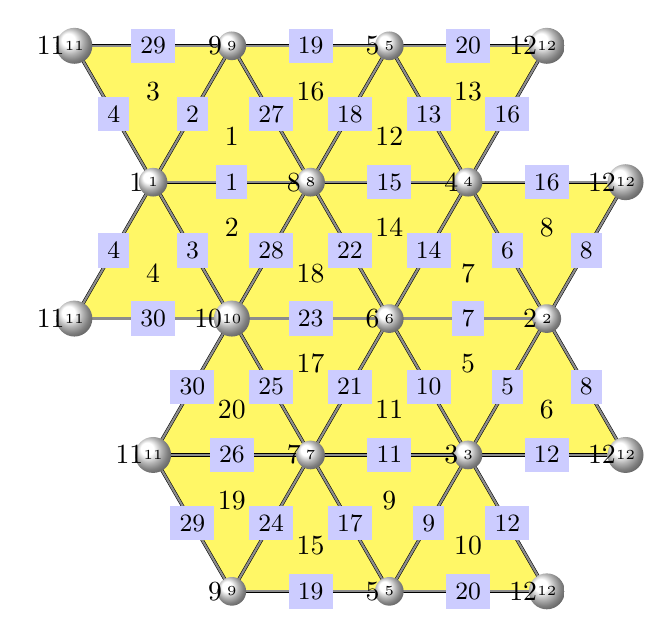
\begin{tikzpicture}[vertexBall, edgeDouble, faceStyle, scale=2]

% Define the coordinates of the vertices
\coordinate (V1_1) at (0, 0);
\coordinate (V2_1) at (2.5, -0.8660254037844385);
\coordinate (V3_1) at (2, -1.732050807568877);
\coordinate (V4_1) at (2, 0);
\coordinate (V5_1) at (1.5, 0.8660254037844387);
\coordinate (V5_2) at (1.5, -2.598076211353316);
\coordinate (V6_1) at (1.5, -0.8660254037844386);
\coordinate (V7_1) at (1, -1.732050807568877);
\coordinate (V8_1) at (1, 0);
\coordinate (V9_1) at (0.4999999999999999, 0.8660254037844386);
\coordinate (V9_2) at (0.5000000000000007, -2.598076211353316);
\coordinate (V10_1) at (0.5000000000000001, -0.8660254037844386);
\coordinate (V11_1) at (-0.5, 0.8660254037844384);
\coordinate (V11_2) at (-0.4999999999999998, -0.8660254037844388);
\coordinate (V11_3) at (0, -1.732050807568878);
\coordinate (V12_1) at (2.5, 0.8660254037844388);
\coordinate (V12_2) at (3, 0);
\coordinate (V12_3) at (3, -1.732050807568877);
\coordinate (V12_4) at (2.5, -2.598076211353316);


% Fill in the faces
\fill[face]  (V8_1) -- (V9_1) -- (V1_1) -- cycle;
\node[faceLabel] at (barycentric cs:V8_1=1,V9_1=1,V1_1=1) {$1$};
\fill[face]  (V1_1) -- (V10_1) -- (V8_1) -- cycle;
\node[faceLabel] at (barycentric cs:V1_1=1,V10_1=1,V8_1=1) {$2$};
\fill[face]  (V9_1) -- (V11_1) -- (V1_1) -- cycle;
\node[faceLabel] at (barycentric cs:V9_1=1,V11_1=1,V1_1=1) {$3$};
\fill[face]  (V1_1) -- (V11_2) -- (V10_1) -- cycle;
\node[faceLabel] at (barycentric cs:V1_1=1,V11_2=1,V10_1=1) {$4$};
\fill[face]  (V6_1) -- (V3_1) -- (V2_1) -- cycle;
\node[faceLabel] at (barycentric cs:V6_1=1,V3_1=1,V2_1=1) {$5$};
\fill[face]  (V3_1) -- (V12_3) -- (V2_1) -- cycle;
\node[faceLabel] at (barycentric cs:V3_1=1,V12_3=1,V2_1=1) {$6$};
\fill[face]  (V6_1) -- (V2_1) -- (V4_1) -- cycle;
\node[faceLabel] at (barycentric cs:V6_1=1,V2_1=1,V4_1=1) {$7$};
\fill[face]  (V2_1) -- (V12_2) -- (V4_1) -- cycle;
\node[faceLabel] at (barycentric cs:V2_1=1,V12_2=1,V4_1=1) {$8$};
\fill[face]  (V7_1) -- (V5_2) -- (V3_1) -- cycle;
\node[faceLabel] at (barycentric cs:V7_1=1,V5_2=1,V3_1=1) {$9$};
\fill[face]  (V5_2) -- (V12_4) -- (V3_1) -- cycle;
\node[faceLabel] at (barycentric cs:V5_2=1,V12_4=1,V3_1=1) {$10$};
\fill[face]  (V6_1) -- (V7_1) -- (V3_1) -- cycle;
\node[faceLabel] at (barycentric cs:V6_1=1,V7_1=1,V3_1=1) {$11$};
\fill[face]  (V8_1) -- (V4_1) -- (V5_1) -- cycle;
\node[faceLabel] at (barycentric cs:V8_1=1,V4_1=1,V5_1=1) {$12$};
\fill[face]  (V4_1) -- (V12_1) -- (V5_1) -- cycle;
\node[faceLabel] at (barycentric cs:V4_1=1,V12_1=1,V5_1=1) {$13$};
\fill[face]  (V8_1) -- (V6_1) -- (V4_1) -- cycle;
\node[faceLabel] at (barycentric cs:V8_1=1,V6_1=1,V4_1=1) {$14$};
\fill[face]  (V7_1) -- (V9_2) -- (V5_2) -- cycle;
\node[faceLabel] at (barycentric cs:V7_1=1,V9_2=1,V5_2=1) {$15$};
\fill[face]  (V8_1) -- (V5_1) -- (V9_1) -- cycle;
\node[faceLabel] at (barycentric cs:V8_1=1,V5_1=1,V9_1=1) {$16$};
\fill[face]  (V6_1) -- (V10_1) -- (V7_1) -- cycle;
\node[faceLabel] at (barycentric cs:V6_1=1,V10_1=1,V7_1=1) {$17$};
\fill[face]  (V8_1) -- (V10_1) -- (V6_1) -- cycle;
\node[faceLabel] at (barycentric cs:V8_1=1,V10_1=1,V6_1=1) {$18$};
\fill[face]  (V7_1) -- (V11_3) -- (V9_2) -- cycle;
\node[faceLabel] at (barycentric cs:V7_1=1,V11_3=1,V9_2=1) {$19$};
\fill[face]  (V10_1) -- (V11_3) -- (V7_1) -- cycle;
\node[faceLabel] at (barycentric cs:V10_1=1,V11_3=1,V7_1=1) {$20$};


% Draw the edges
\draw[edge] (V8_1) -- node[edgeLabel] {$1$} (V1_1);
\draw[edge] (V1_1) -- node[edgeLabel] {$2$} (V9_1);
\draw[edge] (V10_1) -- node[edgeLabel] {$3$} (V1_1);
\draw[edge] (V1_1) -- node[edgeLabel] {$4$} (V11_1);
\draw[edge] (V11_2) -- node[edgeLabel] {$4$} (V1_1);
\draw[edge] (V2_1) -- node[edgeLabel] {$5$} (V3_1);
\draw[edge] (V4_1) -- node[edgeLabel] {$6$} (V2_1);
\draw[edge] (V2_1) -- node[edgeLabel] {$7$} (V6_1);
\draw[edge] (V12_2) -- node[edgeLabel] {$8$} (V2_1);
\draw[edge] (V2_1) -- node[edgeLabel] {$8$} (V12_3);
\draw[edge] (V3_1) -- node[edgeLabel] {$9$} (V5_2);
\draw[edge] (V3_1) -- node[edgeLabel] {$10$} (V6_1);
\draw[edge] (V3_1) -- node[edgeLabel] {$11$} (V7_1);
\draw[edge] (V12_3) -- node[edgeLabel] {$12$} (V3_1);
\draw[edge] (V3_1) -- node[edgeLabel] {$12$} (V12_4);
\draw[edge] (V5_1) -- node[edgeLabel] {$13$} (V4_1);
\draw[edge] (V4_1) -- node[edgeLabel] {$14$} (V6_1);
\draw[edge] (V4_1) -- node[edgeLabel] {$15$} (V8_1);
\draw[edge] (V12_1) -- node[edgeLabel] {$16$} (V4_1);
\draw[edge] (V4_1) -- node[edgeLabel] {$16$} (V12_2);
\draw[edge] (V5_2) -- node[edgeLabel] {$17$} (V7_1);
\draw[edge] (V5_1) -- node[edgeLabel] {$18$} (V8_1);
\draw[edge] (V9_1) -- node[edgeLabel] {$19$} (V5_1);
\draw[edge] (V5_2) -- node[edgeLabel] {$19$} (V9_2);
\draw[edge] (V5_1) -- node[edgeLabel] {$20$} (V12_1);
\draw[edge] (V12_4) -- node[edgeLabel] {$20$} (V5_2);
\draw[edge] (V7_1) -- node[edgeLabel] {$21$} (V6_1);
\draw[edge] (V6_1) -- node[edgeLabel] {$22$} (V8_1);
\draw[edge] (V10_1) -- node[edgeLabel] {$23$} (V6_1);
\draw[edge] (V9_2) -- node[edgeLabel] {$24$} (V7_1);
\draw[edge] (V7_1) -- node[edgeLabel] {$25$} (V10_1);
\draw[edge] (V11_3) -- node[edgeLabel] {$26$} (V7_1);
\draw[edge] (V9_1) -- node[edgeLabel] {$27$} (V8_1);
\draw[edge] (V8_1) -- node[edgeLabel] {$28$} (V10_1);
\draw[edge] (V11_1) -- node[edgeLabel] {$29$} (V9_1);
\draw[edge] (V9_2) -- node[edgeLabel] {$29$} (V11_3);
\draw[edge] (V10_1) -- node[edgeLabel] {$30$} (V11_2);
\draw[edge] (V11_3) -- node[edgeLabel] {$30$} (V10_1);


% Draw the vertices
\vertexLabelR{V1_1}{left}{$1$}
\vertexLabelR{V2_1}{left}{$2$}
\vertexLabelR{V3_1}{left}{$3$}
\vertexLabelR{V4_1}{left}{$4$}
\vertexLabelR{V5_1}{left}{$5$}
\vertexLabelR{V5_2}{left}{$5$}
\vertexLabelR{V6_1}{left}{$6$}
\vertexLabelR{V7_1}{left}{$7$}
\vertexLabelR{V8_1}{left}{$8$}
\vertexLabelR{V9_1}{left}{$9$}
\vertexLabelR{V9_2}{left}{$9$}
\vertexLabelR{V10_1}{left}{$10$}
\vertexLabelR{V11_1}{left}{$11$}
\vertexLabelR{V11_2}{left}{$11$}
\vertexLabelR{V11_3}{left}{$11$}
\vertexLabelR{V12_1}{left}{$12$}
\vertexLabelR{V12_2}{left}{$12$}
\vertexLabelR{V12_3}{left}{$12$}
\vertexLabelR{V12_4}{left}{$12$}

\end{tikzpicture}


\end{center}
 

 Compute elementary properties of \texttt{S} 

 
\begin{Verbatim}[commandchars=!@|,fontsize=\small,frame=single,label=Example]
  !gapprompt@gap>| !gapinput@VertexCounter(S);|
  [ [ 4, 4 ], [ 5, 4 ], [ 6, 4 ] ]
  !gapprompt@gap>| !gapinput@FaceDegreesOfVertices(S);|
  [ 4, 4, 5, 5, 6, 6, 6, 6, 5, 5, 4, 4 ]
\end{Verbatim}
 

 We choose vertex 1 for our examinations and compute the neighbour vertices of
this vertex 

 
\begin{Verbatim}[commandchars=!@|,fontsize=\small,frame=single,label=Example]
  !gapprompt@gap>| !gapinput@NeighbourVerticesOfVertex(S,1);|
  [ 8, 9, 10, 11 ]
\end{Verbatim}
 

 Compute all isosceles coloured surfaces of \texttt{S} 

 
\begin{Verbatim}[commandchars=!@|,fontsize=\small,frame=single,label=Example]
  !gapprompt@gap>| !gapinput@ss:=AllIsoscelesColouredSurfaces(S);|
  [ isosceles coloured surface (12 vertices, 30 edges and 20 faces)
     , isosceles coloured surface (12 vertices, 30 edges and 20 faces)
     , isosceles coloured surface (12 vertices, 30 edges and 20 faces)
     , isosceles coloured surface (12 vertices, 30 edges and 20 faces)
     , isosceles coloured surface (12 vertices, 30 edges and 20 faces)
     , isosceles coloured surface (12 vertices, 30 edges and 20 faces)
     , isosceles coloured surface (12 vertices, 30 edges and 20 faces)
     , isosceles coloured surface (12 vertices, 30 edges and 20 faces)
     , isosceles coloured surface (12 vertices, 30 edges and 20 faces)
     , isosceles coloured surface (12 vertices, 30 edges and 20 faces)
     , isosceles coloured surface (12 vertices, 30 edges and 20 faces)
     , isosceles coloured surface (12 vertices, 30 edges and 20 faces)
     , isosceles coloured surface (12 vertices, 30 edges and 20 faces)
     , isosceles coloured surface (12 vertices, 30 edges and 20 faces) 
   ]
\end{Verbatim}
 

 So introducing the isosceles colouring results in 14 isosceles coloured
surfaces. Display all elementary properties of the first surface in the list \texttt{ss} 

 
\begin{Verbatim}[commandchars=!@|,fontsize=\small,frame=single,label=Example]
  !gapprompt@gap>| !gapinput@Display(ss[1]);|
  Isosceles coloured surface ( closed, orientable, Euler-characteristic 2)
      Vertices (12): [ 1, 2, 3, 4, 5, 6, 7, 8, 9, 10, 11, 12 ]
      Edges (30): [ 1, 2, 3, 4, 5, 6, 7, 8, 9, 10, 11, 12, 13, 14, 15, 16, 17, 18,  
  19, 20, 21, 22, 23, 24, 25, 26, 27, 28, 29, 30 ]
      Faces (20): [ 1, 2, 3, 4, 5, 6, 7, 8, 9, 10, 11, 12, 13, 14, 15, 16, 17, 
  18, 19, 20 ]
      VerticesOfEdges: [ [ 1, 8 ], [ 1, 9 ], [ 1, 10 ], [ 1, 11 ], [ 2, 3 ], 
  [ 2, 4 ], [ 2, 6 ], [ 2, 12 ], [ 3, 5 ], 
  [ 3, 6 ], [ 3, 7 ], [ 3, 12 ],
  [ 4, 5 ], [ 4, 6 ], [ 4, 8 ], [ 4, 12 ], 
  [ 5, 7 ], [ 5, 8 ], [ 5, 9 ], [ 5, 12 ], [ 6, 7 ], [ 6, 8 ], [ 6, 10 ], 
  [ 7, 9 ], [ 7, 10 ], [ 7, 11 ], [ 8, 9 ], [ 8, 10 ], [ 9, 11 ], [ 10, 11 ] ]
     VerticesOfFaces: [ [ 1, 8, 9 ], [ 1, 8, 10 ], [ 1, 9, 11 ], [ 1, 10, 11 ], 
  [ 2, 3, 6 ], [ 2, 3, 12 ], [ 2, 4, 6 ], [ 2, 4, 12 ], [ 3, 5, 7 ], [ 3, 5, 12 ], 
  [ 3, 6, 7 ], [ 4, 5, 8 ], [ 4, 5, 12 ], [ 4, 6, 8 ], [ 5, 7, 9 ], [ 5, 8, 9 ], 
  [ 6, 7, 10 ], [ 6, 8, 10 ], [ 7, 9, 11 ], [ 7, 10, 11 ] ]
      EdgesOfFaces: [ [ 1, 2, 27 ], [ 1, 3, 28 ], [ 2, 4, 29 ],
  [ 3, 4, 30 ], [ 5, 7, 10 ], [ 5, 8, 12 ], [ 6, 7, 14 ], 
  [ 6, 8, 16 ], [ 9, 11, 17 ], [ 9, 12, 20 ], [ 10, 11, 21 ], [ 13, 15, 18 ],
  [ 13, 16, 20 ], [ 14, 15, 22 ], [ 17, 19, 24 ], [ 18, 19, 27 ], [ 21, 23, 25 ], 
  [ 22, 23, 28 ], [ 24, 26, 29 ], [ 25, 26, 30  ]
     Umbrella-paths: [ ( e1, F1, e2, F3, e4, F4, e3, F2, e1 ),
  ( e5, F5, e7, F7, e6, F8, e8, F6, e5 ),
  ( e5, F5, e10, F11, e11, F9, e9, F10, e12, F6, e5 ),
  ( e6, F7, e14, F14, e15, F12, e13, F13, e16, F8, e6 ),
  ( e9, F9, e17, F15, e19, F16, e18, F12, e13, F13, e20, F10, e9 ),
  ( e7, F5, e10, F11, e21, F17, e23, F18, e22, F14, e14, F7, e7 ),
  ( e11, F9, e17, F15, e24, F19, e26, F20, e25, F17, e21, F11, e11 ),
  ( e1, F1, e27, F16, e18, F12, e15, F14, e22, F18, e28, F2, e1 ),
  ( e2, F1, e27, F16, e19, F15, e24, F19, e29, F3, e2 ),
  ( e3, F2, e28, F18, e23, F17, e25, F20, e30, F4, e3 ),
  ( e4, F3, e29, F19, e26, F20, e30, F4, e4 ),
  ( e8, F6, e12, F10, e20, F13, e16, F8, e8 ) ]
     EdgesOfColours: [  [ 1, 2, 3, 4, 5, 6, 8, 9, 10, 11, 13, 14, 18, 19, 20, 22,  
  23, 24, 25, 26 ], [ 7, 12, 15, 16, 17, 21, 27, 28, 29, 30 ] ]
     LocalSymmetry: [ mirror, mirror, mirror, mirror, rotation, rotation, mirror, 
  mirror, rotation, mirror, mirror, mirror, mirror, rotation, mirror, mirror,  
  mirror, mirror, rotation, mirror, mirror, mirror, rotation, rotation, rotation,  
  mirror, mirror, mirror, mirror, mirror ]
\end{Verbatim}
 

 Compute the automorphism group permutating the edges of \texttt{S} 

 
\begin{Verbatim}[commandchars=!@|,fontsize=\small,frame=single,label=Example]
  !gapprompt@gap>| !gapinput@A:=AutomorphismGroupOnEdges(S);|
  Group([ (1,26)(2,29)(3,30)(5,6)(9,13)(10,14)(11,15)(12,16)(17,18)(21,22)
    (24,27)(25,28), (2,3)(5,12)(6,16)(7,20)(9,10)(13,14)(17,21)(18,22)(19,23)
    (24,25)(27,28)(29,30), (1,7)(2,5)(3,6)(4,8)(9,24)(10,27)(11,19)(12,29)
    (13,25)(14,28)(15,23)(16,30)(18,21)(20,26) ])
  !gapprompt@gap>| !gapinput@Size(A);|
  8
\end{Verbatim}
 

 For vertex 1 being an apex, all edges incident to the vertex 1 have to be legs
and the remaining edges of the faces incident to our vertex have to be base
edges. 

 Compute the the edges which have to be base edges 

 
\begin{Verbatim}[commandchars=!@|,fontsize=\small,frame=single,label=Example]
  !gapprompt@gap>| !gapinput@S1:=SubcomplexByFaces(S,FacesOfVertex(S,1));|
  simplicial surface ( 5 vertices, 8 edges, and 4 faces)
  !gapprompt@gap>| !gapinput@bb:=BoundaryEdges(S1);|
  [ 27, 28, 29, 30 ]
\end{Verbatim}
 

 
\begin{center}


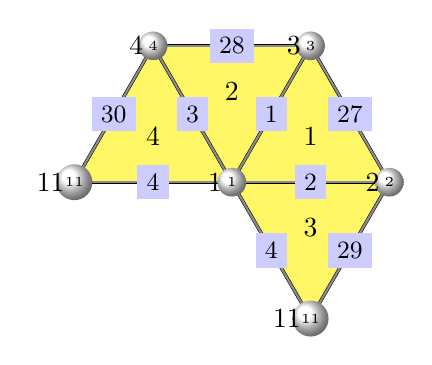
\begin{tikzpicture}[vertexBall, edgeDouble, faceStyle, scale=2]

% Define the coordinates of the vertices
\coordinate (V1_1) at (0, 0);
\coordinate (V2_1) at (1, 0);
\coordinate (V3_1) at (0.4999999999999999, 0.8660254037844386);
\coordinate (V4_1) at (-0.5, 0.8660254037844384);
\coordinate (V5_1) at (0.5000000000000001, -0.8660254037844386);
\coordinate (V5_2) at (-0.9999999999999996, 0);


% Fill in the faces
\fill[face]  (V2_1) -- (V3_1) -- (V1_1) -- cycle;
\node[faceLabel] at (barycentric cs:V2_1=1,V3_1=1,V1_1=1) {$1$};
\fill[face]  (V3_1) -- (V4_1) -- (V1_1) -- cycle;
\node[faceLabel] at (barycentric cs:V3_1=1,V4_1=1,V1_1=1) {$2$};
\fill[face]  (V4_1) -- (V5_2) -- (V1_1) -- cycle;
\node[faceLabel] at (barycentric cs:V4_1=1,V5_2=1,V1_1=1) {$4$};
\fill[face]  (V1_1) -- (V5_1) -- (V2_1) -- cycle;
\node[faceLabel] at (barycentric cs:V1_1=1,V5_1=1,V2_1=1) {$3$};


% Draw the edges
\draw[edge] (V2_1) -- node[edgeLabel] {$2$} (V1_1);
\draw[edge] (V1_1) -- node[edgeLabel] {$1$} (V3_1);
\draw[edge] (V1_1) -- node[edgeLabel] {$3$} (V4_1);
\draw[edge] (V5_1) -- node[edgeLabel] {$4$} (V1_1);
\draw[edge] (V1_1) -- node[edgeLabel] {$4$} (V5_2);
\draw[edge] (V3_1) -- node[edgeLabel] {$27$} (V2_1);
\draw[edge] (V2_1) -- node[edgeLabel] {$29$} (V5_1);
\draw[edge] (V4_1) -- node[edgeLabel] {$28$} (V3_1);
\draw[edge] (V5_2) -- node[edgeLabel] {$30$} (V4_1);


% Draw the vertices
\vertexLabelR{V1_1}{left}{$1$}
\vertexLabelR{V2_1}{left}{$2$}
\vertexLabelR{V3_1}{left}{$3$}
\vertexLabelR{V4_1}{left}{$4$}
\vertexLabelR{V5_1}{left}{$11$}
\vertexLabelR{V5_2}{left}{$11$}

\end{tikzpicture}

\end{center}
 

 Hence we have to find all base-selections containing \texttt{bb} or the set resulting from manipulating bb with the help of an isomorphism of
the automorphism group on the edges. 

 First we have to compute the base-selections of the sufaces in the \texttt{ss}. 
\begin{Verbatim}[commandchars=!@|,fontsize=\small,frame=single,label=Example]
  !gapprompt@gap>| !gapinput@ss:=List(ss,r->Set(List(Faces(r),f->BaseEdgeOfFace(r,f))));|
  [ [ 7, 12, 15, 16, 17, 21, 27, 28, 29, 30 ], 
    [ 7, 8, 15, 17, 20, 21, 27, 28, 29, 30 ], 
    [ 3, 6, 10, 12, 13, 17, 22, 25, 27, 29 ], 
    [ 4, 8, 9, 10, 13, 14, 24, 25, 27, 28 ], 
    [ 4, 7, 12, 15, 16, 17, 21, 26, 27, 28 ], 
    [ 4, 7, 11, 12, 15, 16, 24, 25, 27, 28 ], 
    [ 4, 7, 8, 15, 17, 20, 21, 26, 27, 28 ], 
    [ 4, 7, 8, 11, 15, 20, 24, 25, 27, 28 ], 
    [ 2, 3, 7, 12, 16, 17, 18, 21, 22, 26 ], 
    [ 2, 3, 7, 11, 12, 15, 16, 19, 23, 26 ], 
    [ 2, 3, 7, 8, 17, 18, 20, 21, 22, 26 ], 
    [ 2, 3, 7, 8, 11, 15, 19, 20, 23, 26 ], 
    [ 1, 4, 7, 8, 17, 18, 20, 21, 22, 26 ], 
    [ 1, 4, 7, 8, 11, 15, 19, 20, 23, 26 ] ]
  !gapprompt@gap>| !gapinput@Size(ss);|
  14
\end{Verbatim}
 

 Check whether \texttt{bb} is contained in one of the base selections 

 
\begin{Verbatim}[commandchars=!@|,fontsize=\small,frame=single,label=Example]
  !gapprompt@gap>| !gapinput@obb:=Orbit(A,bb,OnSets);|
  [ [ 27, 28, 29, 30 ], [ 2, 3, 24, 25 ], [ 10, 12, 14, 16 ], [ 5, 6, 9, 13 ] ]
  !gapprompt@gap>| !gapinput@Filtered([1..14],i->IsSubset(ss[i],obb[1]));|
  [ 1, 2 ]
  !gapprompt@gap>| !gapinput@Filtered([1..14],i->IsSubset(ss[i],obb[2]));|
  [  ]
  !gapprompt@gap>| !gapinput@Filtered([1..14],i->IsSubset(ss[i],obb[3]));|
  [  ]
  !gapprompt@gap>| !gapinput@Filtered([1..14],i->IsSubset(ss[i],obb[4]));|
  [  ]
\end{Verbatim}
 

 So at first glance it looks like there are only two possibilities. But there
are more. We obtain this observatin by manipulating the base selection of the
first isoscoles coloured surface in the list \texttt{ss}. 

 
\begin{Verbatim}[commandchars=!@|,fontsize=\small,frame=single,label=Example]
  !gapprompt@gap>| !gapinput@ss1:=Orbit(A,ss[1],OnSets);|
  [ [ 7, 12, 15, 16, 17, 21, 27, 28, 29, 30 ], 
    [ 2, 3, 7, 11, 12, 16, 18, 22, 24, 25 ], 
    [ 5, 6, 15, 17, 20, 21, 27, 28, 29, 30 ], 
    [ 1, 10, 12, 14, 16, 17, 18, 23, 29, 30 ], 
    [ 2, 3, 5, 6, 11, 18, 20, 22, 24, 25 ], 
    [ 1, 5, 6, 9, 13, 19, 21, 22, 29, 30 ], 
    [ 2, 3, 10, 12, 14, 16, 17, 18, 23, 26 ], 
    [ 2, 3, 5, 6, 9, 13, 19, 21, 22, 26 ] ]
  !gapprompt@gap>| !gapinput@Filtered(ss1,r->IsSubset(r,bb));|
  [ [ 7, 12, 15, 16, 17, 21, 27, 28, 29, 30 ], 
    [ 5, 6, 15, 17, 20, 21, 27, 28, 29, 30 ] ]
  !gapprompt@gap>| !gapinput@ss2:=Orbit(A,ss[2],OnSets);|
  [ [ 7, 8, 15, 17, 20, 21, 27, 28, 29, 30 ], 
    [ 2, 3, 7, 8, 11, 18, 20, 22, 24, 25 ], 
    [ 1, 4, 10, 12, 14, 16, 17, 18, 23, 26 ], 
    [ 1, 4, 5, 6, 9, 13, 19, 21, 22, 26 ] ]
  !gapprompt@gap>| !gapinput@Filtered(ss2,r->IsSubset(r,bb));|
  [ [ 7, 8, 15, 17, 20, 21, 27, 28, 29, 30 ] ]
\end{Verbatim}
 

 Hence we have at least three possibilities for an isosceles coloured
simplicial suface resulting from \texttt{S} and having vertex 1 as apex. Indeed there exactly three such surfaces. Let us
now visualise these edge coloured surfaces. 

 Compute the isosceles coloured surfaces with the constructed base selections 
\begin{Verbatim}[commandchars=!@|,fontsize=\small,frame=single,label=Example]
  !gapprompt@gap>| !gapinput@SS1:=List([1..30],i->1);|
  [ 1, 1, 1, 1, 1, 1, 1, 1, 1, 1, 1, 1, 1, 1, 1, 1, 1, 1, 1, 1, 1, 1, 1, 1, 1, 
   1, 1, 1, 1, 1 ]
  !gapprompt@gap>| !gapinput@for i in ss1[1] do SS1[i]:=2;od;|
  !gapprompt@gap>| !gapinput@SS1:=EdgeColouredPolygonalComplex(S,SS1);|
  isosceles coloured surface (12 vertices, 30 edges and 20 faces)
  !gapprompt@gap>| !gapinput@SS2:=List([1..30],i->1);|
  [ 1, 1, 1, 1, 1, 1, 1, 1, 1, 1, 1, 1, 1, 1, 1, 1, 1, 1, 1, 1, 1, 1, 1, 1, 1, 
    1, 1, 1, 1, 1 ]
  !gapprompt@gap>| !gapinput@for i in ss1[3] do SS2[i]:=2;od;|
  !gapprompt@gap>| !gapinput@SS2:=EdgeColouredPolygonalComplex(S,SS2);|
  isosceles coloured surface (12 vertices, 30 edges and 20 faces)
  !gapprompt@gap>| !gapinput@SS3:=List([1..30],i->1);|
  [ 1, 1, 1, 1, 1, 1, 1, 1, 1, 1, 1, 1, 1, 1, 1, 1, 1, 1, 1, 1, 1, 1, 1, 1, 1, 
    1, 1, 1, 1, 1 ]
  !gapprompt@gap>| !gapinput@for i in ss2[1] do SS3[i]:=2;od;|
  !gapprompt@gap>| !gapinput@SS3:=EdgeColouredPolygonalComplex(S,SS3);|
  isosceles coloured surface (12 vertices, 30 edges and 20 faces)
\end{Verbatim}
 

 Draw the net of the surface \texttt{SS1} into a tex-file using TikZ 

 
\begin{Verbatim}[commandchars=!@|,fontsize=\small,frame=single,label=Example]
  !gapprompt@gap>| !gapinput@pr:=rec(edgeColourClassColours:=["red","blue"],|
  !gapprompt@>| !gapinput@edgeColourClassLengths:=[1.2, 0.8]);;|
  !gapprompt@gap>| !gapinput@pr.compileLaTeX:=true;|
  true
  !gapprompt@gap>| !gapinput@pr:=DrawSurfaceToTikz(SS1,"Zwa1",pr);;|
  DrawSurfaceToTikz: Could not find intersection-free continuation. Draw face 
  17 via edge 21 instead.
  Picture written in TikZ.Start LaTeX-compilation (type 'x' and press ENTER to
  abort).
  Picture rendered (with pdflatex).
\end{Verbatim}
 

 
\begin{center}
            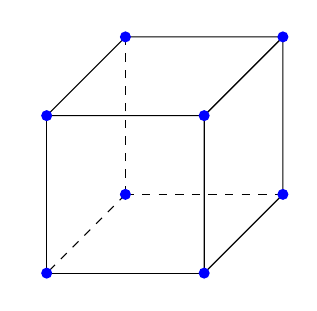
\begin{tikzpicture}[vertexStyle=nolabels, edgeStyle=nolabels]
                % We need to define the drawing style

                \coordinate (FDL) at (0,0); % front down left
                \coordinate (FDR) at (2,0); % front down right
                \coordinate (FUL) at (0,2); % front up left
                \coordinate (BDL) at (1,1); % back up left
                \coordinate (BDR) at ($(FDR)+(BDL)$); % back down right
                \coordinate (FUR) at ($(FUL)+(FDR)$); % front up right
                \coordinate (BUL) at ($(FUL)+(BDL)$); % back up left
                \coordinate (BUR) at ($(FDR)+(FUL)+(BDL)$); % back up right

                % Draw the edges
                \foreach \x in {FDL, BDR, BUL}{
                    \draw[dashed, edge] (BDL) -- (\x);
                }


                \draw[edge] (FDL) -- (FDR) -- (FUR) -- (FUL) -- cycle;
                \draw[edge] (FDR) -- (BDR) -- (BUR) -- (FUR) -- cycle;
                \draw[edge] (FUL) -- (FUR) -- (BUR) -- (BUL) -- cycle;

                % Draw the vertices
                \foreach \x in {FDL, FDR, FUL, BDL, BDR, FUR, BUL, BUR} {
                    \vertexLabelR{\x}{left}{}
                }
            \end{tikzpicture}


\end{center}
 

 Draw the net of the surface \texttt{SS2} into a tex-file using TikZ 

 
\begin{Verbatim}[commandchars=!@|,fontsize=\small,frame=single,label=Example]
  !gapprompt@gap>| !gapinput@pr:=rec(edgeColourClassColours:=["red","blue"],|
  !gapprompt@>| !gapinput@edgeColourClassLengths:=[1.2, 0.8], compileLaTeX:=true);;|
  !gapprompt@gap>| !gapinput@pr:=DrawSurfaceToTikz(SS2,"Zwa2",pr);;|
  DrawSurfaceToTikz: Could not find intersection-free continuation. Draw face 
  18 via edge 22 instead.
  Picture written in TikZ.Start LaTeX-compilation (type 'x' and press ENTER to
  abort).
  Picture rendered (with pdflatex).
\end{Verbatim}
 

 
\begin{center}
            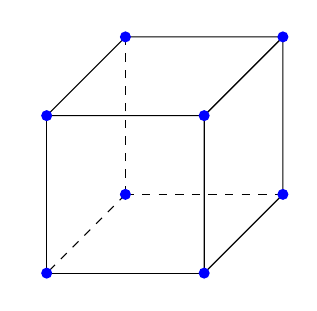
\begin{tikzpicture}[vertexStyle=nolabels, edgeStyle=nolabels]
                % We need to define the drawing style

                \coordinate (FDL) at (0,0); % front down left
                \coordinate (FDR) at (2,0); % front down right
                \coordinate (FUL) at (0,2); % front up left
                \coordinate (BDL) at (1,1); % back up left
                \coordinate (BDR) at ($(FDR)+(BDL)$); % back down right
                \coordinate (FUR) at ($(FUL)+(FDR)$); % front up right
                \coordinate (BUL) at ($(FUL)+(BDL)$); % back up left
                \coordinate (BUR) at ($(FDR)+(FUL)+(BDL)$); % back up right

                % Draw the edges
                \foreach \x in {FDL, BDR, BUL}{
                    \draw[dashed, edge] (BDL) -- (\x);
                }


                \draw[edge] (FDL) -- (FDR) -- (FUR) -- (FUL) -- cycle;
                \draw[edge] (FDR) -- (BDR) -- (BUR) -- (FUR) -- cycle;
                \draw[edge] (FUL) -- (FUR) -- (BUR) -- (BUL) -- cycle;

                % Draw the vertices
                \foreach \x in {FDL, FDR, FUL, BDL, BDR, FUR, BUL, BUR} {
                    \vertexLabelR{\x}{left}{}
                }
            \end{tikzpicture}


\end{center}
 

 Draw the net of the surface \texttt{SS3} into a tex-file using TikZ 

 
\begin{Verbatim}[commandchars=!@|,fontsize=\small,frame=single,label=Example]
  !gapprompt@gap>| !gapinput@pr:=rec(edgeColourClassColours:=["red","blue"],|
  !gapprompt@>| !gapinput@edgeColourClassLengths:=[1.2, 0.8], compileLaTeX:=true);;|
  !gapprompt@gap>| !gapinput@pr:=DrawSurfaceToTikz(SS3,"Zwa3",pr);;|
  DrawSurfaceToTikz: Could not find intersection-free continuation. Draw face 
  17 via edge 21 instead.
  Picture written in TikZ.Start LaTeX-compilation (type 'x' and press ENTER to
  abort).
  Picture rendered (with pdflatex).
\end{Verbatim}
 

 
\begin{center}
            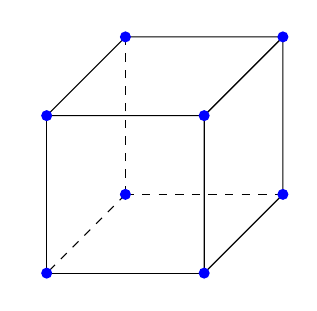
\begin{tikzpicture}[vertexStyle=nolabels, edgeStyle=nolabels]
                % We need to define the drawing style

                \coordinate (FDL) at (0,0); % front down left
                \coordinate (FDR) at (2,0); % front down right
                \coordinate (FUL) at (0,2); % front up left
                \coordinate (BDL) at (1,1); % back up left
                \coordinate (BDR) at ($(FDR)+(BDL)$); % back down right
                \coordinate (FUR) at ($(FUL)+(FDR)$); % front up right
                \coordinate (BUL) at ($(FUL)+(BDL)$); % back up left
                \coordinate (BUR) at ($(FDR)+(FUL)+(BDL)$); % back up right

                % Draw the edges
                \foreach \x in {FDL, BDR, BUL}{
                    \draw[dashed, edge] (BDL) -- (\x);
                }


                \draw[edge] (FDL) -- (FDR) -- (FUR) -- (FUL) -- cycle;
                \draw[edge] (FDR) -- (BDR) -- (BUR) -- (FUR) -- cycle;
                \draw[edge] (FUL) -- (FUR) -- (BUR) -- (BUL) -- cycle;

                % Draw the vertices
                \foreach \x in {FDL, FDR, FUL, BDL, BDR, FUR, BUL, BUR} {
                    \vertexLabelR{\x}{left}{}
                }
            \end{tikzpicture}


\end{center}
 

 }

 
\section{\textcolor{Chapter }{Butterfly-Deletion}}\label{Section_Butterfly-Deletion}
\logpage{[ 3, 5, 0 ]}
\hyperdef{L}{X871CFBF77CD6FB71}{}
{
  

 $Problems:$ Construction of spheres via butterfly-deletions on the icosahedron 

 $Theoretical$ $background$ 
\begin{itemize}
\item  Vertex-faithful surfaces and boolean operations 
\item  Umbrella descriptor of simplicial surfaces 
\end{itemize}
 

 $Frequently$ $used$ $commands$ 
\begin{itemize}
\item  AutomorphismGroupOnFaces() (\ref{AutomorphismGroupOnFaces}) 
\item  UmbrellaDescriptorOfSurface() (\ref{UmbrellaDescriptorOfSurface}) 
\end{itemize}
 

 $Less$ $frequently$ $used$ $commands$ 
\begin{itemize}
\item  Icosahedron() (\ref{Icosahedron}) 
\item  DistanceOfFaces() (\ref{DistanceOfFaces}) 
\end{itemize}
 $ Mathematical$ $details:$ The butterfly deletion constructs a simplicial surface by removing a butterfly
of a given simplicial surface. To apply the butterfly deletion we need an
inner edge of the surface not belonging to a 2-Waist. The resulting simplicial
surface can be defined in two steps. 
\begin{enumerate}
\item  The two faces incident to the given inner edge are removed from the surface by
applying cuts along the four edges incident to exactly one of the two faces. 
\item  Step 1 gives rise to four new boundary edges and two boundary vertices which
were incident to exactly one of the removed faces. By applying mender
operations so that each pair of edges incident to the same boundary vertex get
identified, the simplicial surfac resulting from the butterfly deletion is
constructed. 
\end{enumerate}
 Clearly the butterfly deletion can be reversed, namely by using the butterfly
insertion. 

 
\begin{center}
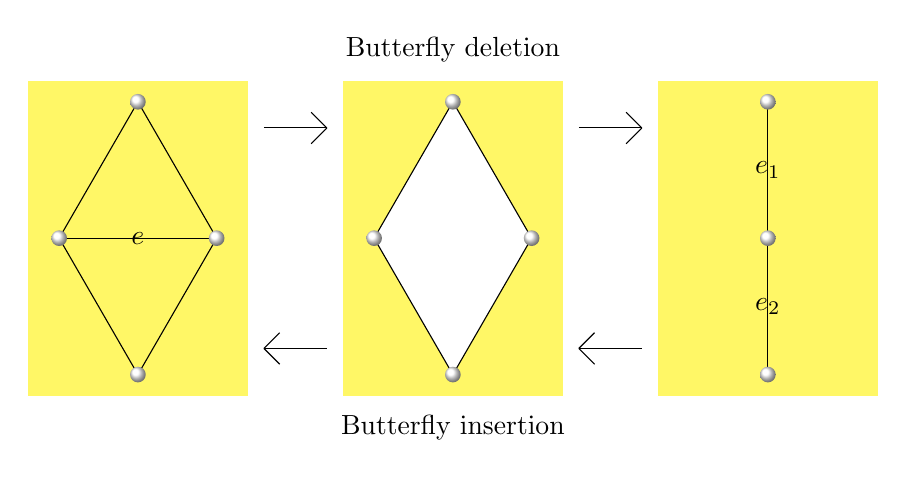
\begin{tikzpicture}[vertexBall,edgeDouble,faceStyle, edgeStyle=nolabels, scale=2]


% Define the coordinates of the vertices

\coordinate (V1_1) at (0, 0);

\coordinate (V2_1) at (1, 0);

\coordinate (V3_1) at (0.5, 0.8660254037844386);

\coordinate (V4_1) at (0.5, -0.8660254037844386);


\coordinate (V1_2) at (2, 0);

\coordinate (V2_2) at (3, 0);

\coordinate (V3_2) at (2.5, 0.8660254037844386);

\coordinate (V4_2) at (2.5, -0.8660254037844386);


\coordinate (V3_3) at (4.5, 0.8660254037844386);

\coordinate (V4_3) at (4.5, -0.8660254037844386);

\coordinate (V) at (4.5, 0);

% Fill in the faces

\fill[face]  (-0.2,-1) -- (-0.2,1) -- (1.2,1)--(1.2,-1) -- cycle;

\fill[face]  (1.8,-1) -- (1.8,1) -- (3.2,1)--(3.2,-1) -- cycle;

\fill[face]  (3.8,-1) -- (3.8,1) -- (5.2,1)--(5.2,-1) -- cycle;

\fill[face]  (V2_1) -- (V3_1) -- (V1_1) -- cycle;

%\node[faceLabel] at (barycentric cs:V2_1=1,V3_1=1,V1_1=1) {$F_1$};

\fill[face]  (V2_1) -- (V4_1) -- (V1_1) -- cycle;

%\node[faceLabel] at (barycentric cs:V2_1=1,V4_1=1,V1_1=1) {$F_2$};


\fill[face=white]  (V2_2) -- (V3_2) -- (V1_2) -- cycle;

%\node[faceLabel] at (barycentric cs:V2_1=1,V3_1=1,V1_1=1) {$F_1$};

\fill[face=white]  (V2_2) -- (V4_2) -- (V1_2) -- cycle;

%\node[faceLabel] at (barycentric cs:V2_1=1,V4_1=1,V1_1=1) {$F_2$};

% Draw the edges

\draw[edge] (V2_1) -- node[edgeLabel] {$e$} (V1_1);

\draw[edge] (V1_1) --  (V3_1);

\draw[edge] (V3_1) --  (V2_1);

\draw[edge] (V4_1) --  (V2_1);

\draw[edge] (V4_1) --  (V1_1);


%\draw[edge] (V2_2) -- node[edgeLabel] {$e_1$} (V1_2);

\draw[edge] (V1_2) --  (V3_2);

\draw[edge] (V3_2) -- (V2_2);

\draw[edge] (V4_2) -- (V2_2);

\draw[edge] (V4_2) --  (V1_2);



\draw[edge] (V) -- node[edgeLabel] {$e_1$} (V3_3);

\draw[edge] (V4_3) -- node[edgeLabel] {$e_2$} (V);

\draw[edge] (1.3,0.7) -- (1.7,0.7);

\draw[edge] (1.6,0.7-0.1) -- (1.7,0.7);

\draw[edge] (1.6,0.7+.1) -- (1.7,0.7);


\draw[edge] (3.3,0.7) -- (3.7,0.7);

\draw[edge] (3.6,0.7-0.1) -- (3.7,0.7);

\draw[edge] (3.6,0.7+.1) -- (3.7,0.7);


\draw[edge] (1.3,-0.7) -- (1.7,-0.7);

\draw[edge] (1.4,-0.7-0.1) -- (1.3,-0.7);

\draw[edge] (1.4,-0.7+.1) -- (1.3,-0.7);


\draw[edge] (3.3,-0.7) -- (3.7,-0.7);

\draw[edge] (3.4,-0.7-0.1) -- (3.3,-0.7);

\draw[edge] (3.4,-0.7+.1) -- (3.3,-0.7);

\node[faceLabel] at (2.5,-1.2) {Butterfly insertion};

\node[faceLabel] at (2.5,1.2) {Butterfly deletion};

% Draw the vertices

\vertexLabelR{V1_1}{left}{$ $}

\vertexLabelR{V2_1}{left}{$ $}

\vertexLabelR{V3_1}{left}{$ $}

\vertexLabelR{V4_1}{left}{$ $}


\vertexLabelR{V1_2}{left}{$ $}

\vertexLabelR{V2_2}{left}{$ $}

\vertexLabelR{V3_2}{left}{$ $}

\vertexLabelR{V4_2}{left}{$ $}


\vertexLabelR{V3_3}{left}{$ $}

\vertexLabelR{V4_3}{left}{$ $}


\vertexLabelR{V}{left}{$ $}

\end{tikzpicture}


\end{center}
 

 In this chapter we will familliarize ourselves with the butterfly deletion. We
want to compute the simplicial surfaces constructed up to isomorphism by
applying at most two butterfly deletions to the icosahedron. Note, applying
the butterfly deletion to a simplicial surface does not affect the
Euler-Characteristic. 

 
%\begin{center}
%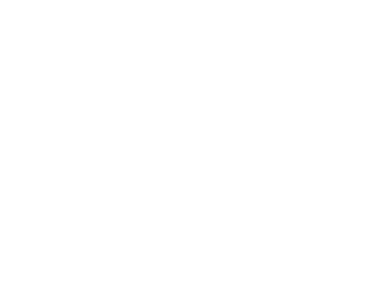
\includegraphics{tikzpictures/Ico.png}
%\end{center}
 

 Since a given simplicial surface can be uniquly reconstructed from it's
umbrella descriptor, we shall use this structure to examine the butterfly
deletion in this exercise. Note, it is also possible to define this
construction by manipulating the incidence structure, namely the edges of
faces and the vertices of edges. 

 Let us start by defining a function that omits a given face from a simplicial
surface represented by its umbrella descriptor. 

 
\begin{center}
% header missing

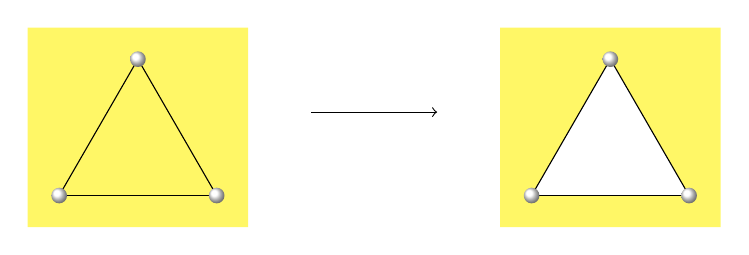
\begin{tikzpicture}[vertexBall,edgeDouble,faceStyle, edgeStyle=nolabels, scale=2]
%%%%
\coordinate (V0) at (0.,0.);
\coordinate (V1) at (1.,0.);
\coordinate (V2) at (.5,0.866);
\fill[face]  ($(V0)-(0.2,0.2)$) -- ($(V1)+(0.2,-0.2)$) -- ($(V2)+(0.7,0.2)$) --($(V2)-(0.7,-0.2)$) -- cycle;
\fill[face]  ($(V0)-(0.2,0.2)+(3.,0.)$) -- ($(V1)+(0.2,-0.2)+(3.,0.)$) -- ($(V2)+(0.7,0.2)+(3.,0.)$) --($(V2)-(0.7,-0.2)+(3.,0.)$) -- cycle;

\fill[face=white]  ($(V0)+(3.,0.)$) -- ($(V1)+(3.,0.)$) -- ($(V2)+(3.,0.)$) -- cycle;
\draw[->] (1.6,0.53) -- (2.4,0.53);


\draw[edge] (V0) -- (V1);
\draw[edge] (V1) -- (V2);
\draw[edge] (V0) -- (V2);

\draw[edge] ($(V0)+(3.,0.)$) -- ($(V1)+(3.,0.)$);
\draw[edge] ($(V1)+(3.,0.)$) -- ($(V2)+(3.,0.)$);
\draw[edge] ($(V0)+(3.,0.)$) -- ($(V2)+(3.,0.)$);
\vertexLabelR{V0}{below}{$ $}
\vertexLabelR{V1}{below}{$ $}
\vertexLabelR{V2}{below}{$ $}

\vertexLabelR{$(V0) +(3.,0.)$}{below}{$ $}
\vertexLabelR{$(V1) +(3.,0.)$}{below}{$ $}
\vertexLabelR{$(V2) +(3.,0.)$}{below}{$ $}
\end{tikzpicture}
%\end{document}

\end{center}
 

 
\begin{Verbatim}[commandchars=!@|,fontsize=\small,frame=single,label=Example]
  !gapprompt@gap>| !gapinput@Omit:=function ( Z, i )|
     local a, b;
     if i ^ Z = i then
         return Z;
     fi;
     a := Orbit( Group( Z ), i );
     b := List( [ 2 .. Size( a ) ], function ( i )
             return a[i];
         end );
     return CycleFromList( b );
  end
\end{Verbatim}
 

 Given the umbrella descriptor of a simplicial surface, the butterfly deletion
can be applied by using the folllowing function. 

 
\begin{Verbatim}[commandchars=!@|,fontsize=\small,frame=single,label=Example]
  gap>Zus:=function ( ZZ, i, j )
      local ZZ1, r, k;
      ZZ1 := Filtered( ZZ, function ( r )
              return not (i ^ r = j or j ^ r = i);
         end );
      ZZ1 := List( ZZ1, function ( r )
             return Omit( r, i );
         end );
     ZZ1 := List( ZZ1, function ( r )
             return Omit( r, j );
          end );
      r := Filtered( ZZ, function ( r )
              return i ^ r = j or j ^ r = i;
          end );
      if i ^ r[1] <> j then
          r[1] := r[1] ^ -1;
      fi;
      if j ^ r[2] <> i then
          r[2] := r[2] ^ -1;
      fi;
      r[1] := Orbit( Group( r[1] ), i );
      r[2] := Orbit( Group( r[2] ), j );
      r[1] := List( [ 3 .. Size( r[1] ) ], function ( k )
              return r[1][k];
          end );
      r[2] := List( [ 3 .. Size( r[2] ) ], function ( k )
              return r[2][k];
          end );
      for k in r[2] do
          Add( r[1], k );
      od;
      Add( ZZ1, CycleFromList( r[1] ) );
      return ZZ1;
  end
\end{Verbatim}
 

 Let us compute the icosahedron and it's umbrella descriptor. 

 
\begin{Verbatim}[commandchars=!@|,fontsize=\small,frame=single,label=Example]
  !gapprompt@gap>| !gapinput@Ik:=Icosahedron();|
  simplicial surface (12 vertices, 30 edges, and 20 faces)
  !gapprompt@gap>| !gapinput@UIk:=UmbrellaDescriptorOfSurface(Ik);|
  [ (1,5,4,3,2), (1,6,11,7,2), (1,6,15,10,5), (2,7,12,8,3), (3,8,13,9,4), 
    (4,9,14,10,5), (6,15,20,16,11), (7,12,17,16,11), (8,13,18,17,12), 
    (9,14,19,18,13), (10,14,19,20,15), (16,17,18,19,20) ]
\end{Verbatim}
 

 
\begin{center}
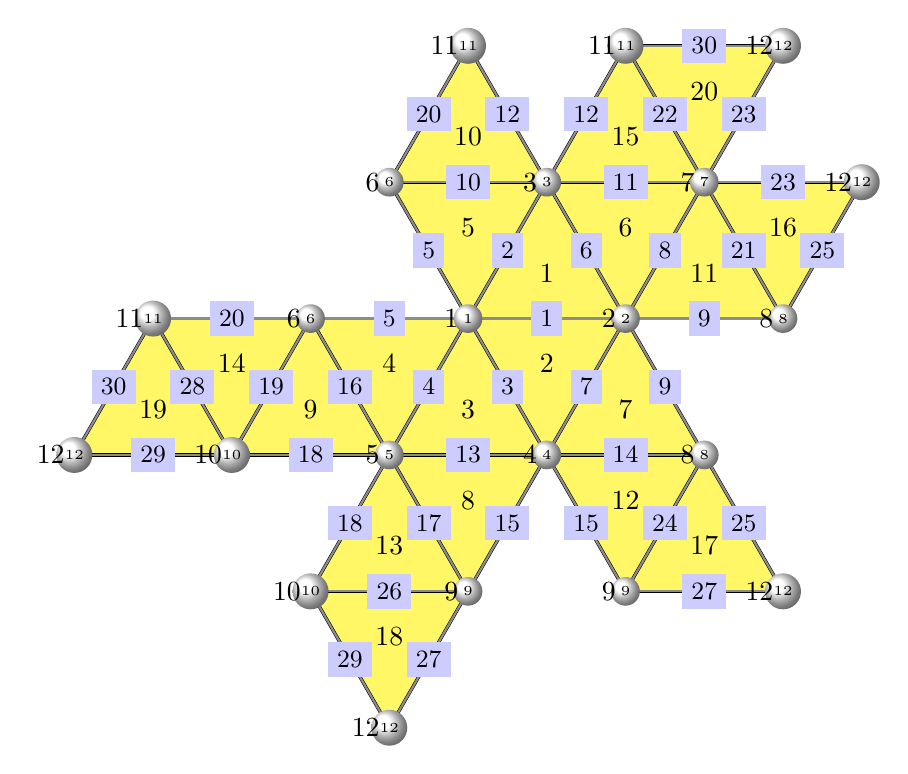
\begin{tikzpicture}[vertexBall, edgeDouble, faceStyle, scale=2]

% Define the coordinates of the vertices
\coordinate (V1_1) at (0., 0.);
\coordinate (V2_1) at (1., 0.);
\coordinate (V3_1) at (0.4999999999999999, 0.8660254037844386);
\coordinate (V4_1) at (0.5000000000000001, -0.8660254037844386);
\coordinate (V5_1) at (-0.4999999999999998, -0.8660254037844388);
\coordinate (V6_1) at (-0.5, 0.8660254037844384);
\coordinate (V6_2) at (-1., 0.);
\coordinate (V7_1) at (1.5, 0.8660254037844388);
\coordinate (V8_1) at (1.5, -0.8660254037844384);
\coordinate (V8_2) at (2., 0.);
\coordinate (V9_1) at (0., -1.732050807568877);
\coordinate (V9_2) at (1., -1.732050807568877);
\coordinate (V10_1) at (-1.5, -0.866025403784439);
\coordinate (V10_2) at (-0.9999999999999996, -1.732050807568877);
\coordinate (V11_1) at (0., 1.732050807568877);
\coordinate (V11_2) at (0.9999999999999996, 1.732050807568877);
\coordinate (V11_3) at (-2., 0.);
\coordinate (V12_1) at (2.5, 0.866025403784439);
\coordinate (V12_2) at (1.999999999999999, 1.732050807568877);
\coordinate (V12_3) at (2., -1.732050807568877);
\coordinate (V12_4) at (-0.4999999999999997, -2.598076211353316);
\coordinate (V12_5) at (-2.5, -0.8660254037844393);


% Fill in the faces
\fill[face]  (V2_1) -- (V3_1) -- (V1_1) -- cycle;
\node[faceLabel] at (barycentric cs:V2_1=1,V3_1=1,V1_1=1) {$1$};
\fill[face]  (V1_1) -- (V4_1) -- (V2_1) -- cycle;
\node[faceLabel] at (barycentric cs:V1_1=1,V4_1=1,V2_1=1) {$2$};
\fill[face]  (V1_1) -- (V5_1) -- (V4_1) -- cycle;
\node[faceLabel] at (barycentric cs:V1_1=1,V5_1=1,V4_1=1) {$3$};
\fill[face]  (V1_1) -- (V6_2) -- (V5_1) -- cycle;
\node[faceLabel] at (barycentric cs:V1_1=1,V6_2=1,V5_1=1) {$4$};
\fill[face]  (V3_1) -- (V6_1) -- (V1_1) -- cycle;
\node[faceLabel] at (barycentric cs:V3_1=1,V6_1=1,V1_1=1) {$5$};
\fill[face]  (V2_1) -- (V7_1) -- (V3_1) -- cycle;
\node[faceLabel] at (barycentric cs:V2_1=1,V7_1=1,V3_1=1) {$6$};
\fill[face]  (V4_1) -- (V8_1) -- (V2_1) -- cycle;
\node[faceLabel] at (barycentric cs:V4_1=1,V8_1=1,V2_1=1) {$7$};
\fill[face]  (V5_1) -- (V9_1) -- (V4_1) -- cycle;
\node[faceLabel] at (barycentric cs:V5_1=1,V9_1=1,V4_1=1) {$8$};
\fill[face]  (V6_2) -- (V10_1) -- (V5_1) -- cycle;
\node[faceLabel] at (barycentric cs:V6_2=1,V10_1=1,V5_1=1) {$9$};
\fill[face]  (V3_1) -- (V11_1) -- (V6_1) -- cycle;
\node[faceLabel] at (barycentric cs:V3_1=1,V11_1=1,V6_1=1) {$10$};
\fill[face]  (V2_1) -- (V8_2) -- (V7_1) -- cycle;
\node[faceLabel] at (barycentric cs:V2_1=1,V8_2=1,V7_1=1) {$11$};
\fill[face]  (V4_1) -- (V9_2) -- (V8_1) -- cycle;
\node[faceLabel] at (barycentric cs:V4_1=1,V9_2=1,V8_1=1) {$12$};
\fill[face]  (V5_1) -- (V10_2) -- (V9_1) -- cycle;
\node[faceLabel] at (barycentric cs:V5_1=1,V10_2=1,V9_1=1) {$13$};
\fill[face]  (V6_2) -- (V11_3) -- (V10_1) -- cycle;
\node[faceLabel] at (barycentric cs:V6_2=1,V11_3=1,V10_1=1) {$14$};
\fill[face]  (V7_1) -- (V11_2) -- (V3_1) -- cycle;
\node[faceLabel] at (barycentric cs:V7_1=1,V11_2=1,V3_1=1) {$15$};
\fill[face]  (V8_2) -- (V12_1) -- (V7_1) -- cycle;
\node[faceLabel] at (barycentric cs:V8_2=1,V12_1=1,V7_1=1) {$16$};
\fill[face]  (V9_2) -- (V12_3) -- (V8_1) -- cycle;
\node[faceLabel] at (barycentric cs:V9_2=1,V12_3=1,V8_1=1) {$17$};
\fill[face]  (V10_2) -- (V12_4) -- (V9_1) -- cycle;
\node[faceLabel] at (barycentric cs:V10_2=1,V12_4=1,V9_1=1) {$18$};
\fill[face]  (V11_3) -- (V12_5) -- (V10_1) -- cycle;
\node[faceLabel] at (barycentric cs:V11_3=1,V12_5=1,V10_1=1) {$19$};
\fill[face]  (V7_1) -- (V12_2) -- (V11_2) -- cycle;
\node[faceLabel] at (barycentric cs:V7_1=1,V12_2=1,V11_2=1) {$20$};


% Draw the edges
\draw[edge] (V2_1) -- node[edgeLabel] {$1$} (V1_1);
\draw[edge] (V1_1) -- node[edgeLabel] {$2$} (V3_1);
\draw[edge] (V4_1) -- node[edgeLabel] {$3$} (V1_1);
\draw[edge] (V5_1) -- node[edgeLabel] {$4$} (V1_1);
\draw[edge] (V1_1) -- node[edgeLabel] {$5$} (V6_1);
\draw[edge] (V6_2) -- node[edgeLabel] {$5$} (V1_1);
\draw[edge] (V3_1) -- node[edgeLabel] {$6$} (V2_1);
\draw[edge] (V2_1) -- node[edgeLabel] {$7$} (V4_1);
\draw[edge] (V7_1) -- node[edgeLabel] {$8$} (V2_1);
\draw[edge] (V2_1) -- node[edgeLabel] {$9$} (V8_1);
\draw[edge] (V8_2) -- node[edgeLabel] {$9$} (V2_1);
\draw[edge] (V6_1) -- node[edgeLabel] {$10$} (V3_1);
\draw[edge] (V3_1) -- node[edgeLabel] {$11$} (V7_1);
\draw[edge] (V11_1) -- node[edgeLabel] {$12$} (V3_1);
\draw[edge] (V3_1) -- node[edgeLabel] {$12$} (V11_2);
\draw[edge] (V4_1) -- node[edgeLabel] {$13$} (V5_1);
\draw[edge] (V8_1) -- node[edgeLabel] {$14$} (V4_1);
\draw[edge] (V4_1) -- node[edgeLabel] {$15$} (V9_1);
\draw[edge] (V9_2) -- node[edgeLabel] {$15$} (V4_1);
\draw[edge] (V5_1) -- node[edgeLabel] {$16$} (V6_2);
\draw[edge] (V9_1) -- node[edgeLabel] {$17$} (V5_1);
\draw[edge] (V5_1) -- node[edgeLabel] {$18$} (V10_1);
\draw[edge] (V10_2) -- node[edgeLabel] {$18$} (V5_1);
\draw[edge] (V10_1) -- node[edgeLabel] {$19$} (V6_2);
\draw[edge] (V6_1) -- node[edgeLabel] {$20$} (V11_1);
\draw[edge] (V11_3) -- node[edgeLabel] {$20$} (V6_2);
\draw[edge] (V7_1) -- node[edgeLabel] {$21$} (V8_2);
\draw[edge] (V11_2) -- node[edgeLabel] {$22$} (V7_1);
\draw[edge] (V7_1) -- node[edgeLabel] {$23$} (V12_1);
\draw[edge] (V12_2) -- node[edgeLabel] {$23$} (V7_1);
\draw[edge] (V8_1) -- node[edgeLabel] {$24$} (V9_2);
\draw[edge] (V12_1) -- node[edgeLabel] {$25$} (V8_2);
\draw[edge] (V8_1) -- node[edgeLabel] {$25$} (V12_3);
\draw[edge] (V9_1) -- node[edgeLabel] {$26$} (V10_2);
\draw[edge] (V12_3) -- node[edgeLabel] {$27$} (V9_2);
\draw[edge] (V9_1) -- node[edgeLabel] {$27$} (V12_4);
\draw[edge] (V10_1) -- node[edgeLabel] {$28$} (V11_3);
\draw[edge] (V12_4) -- node[edgeLabel] {$29$} (V10_2);
\draw[edge] (V10_1) -- node[edgeLabel] {$29$} (V12_5);
\draw[edge] (V11_2) -- node[edgeLabel] {$30$} (V12_2);
\draw[edge] (V12_5) -- node[edgeLabel] {$30$} (V11_3);


% Draw the vertices
\vertexLabelR{V1_1}{left}{$1$}
\vertexLabelR{V2_1}{left}{$2$}
\vertexLabelR{V3_1}{left}{$3$}
\vertexLabelR{V4_1}{left}{$4$}
\vertexLabelR{V5_1}{left}{$5$}
\vertexLabelR{V6_1}{left}{$6$}
\vertexLabelR{V6_2}{left}{$6$}
\vertexLabelR{V7_1}{left}{$7$}
\vertexLabelR{V8_1}{left}{$8$}
\vertexLabelR{V8_2}{left}{$8$}
\vertexLabelR{V9_1}{left}{$9$}
\vertexLabelR{V9_2}{left}{$9$}
\vertexLabelR{V10_1}{left}{$10$}
\vertexLabelR{V10_2}{left}{$10$}
\vertexLabelR{V11_1}{left}{$11$}
\vertexLabelR{V11_2}{left}{$11$}
\vertexLabelR{V11_3}{left}{$11$}
\vertexLabelR{V12_1}{left}{$12$}
\vertexLabelR{V12_2}{left}{$12$}
\vertexLabelR{V12_3}{left}{$12$}
\vertexLabelR{V12_4}{left}{$12$}
\vertexLabelR{V12_5}{left}{$12$}

\end{tikzpicture}

\end{center}
 

 Up to isomorphism there is exactly one sphere resulting from applying exactly
one butterfly deletion to the icosahedron. We obtain this sphere represented
by it's umbrella descriptor by removing the butterfly containing the faces 1
and 2. 

 
\begin{Verbatim}[commandchars=!@|,fontsize=\small,frame=single,label=Example]
  !gapprompt@gap>| !gapinput@U1:=Zus(UIK,1,2);|
  [ (5,6,15,10), (3,7,12,8), (3,8,13,9,4), (4,9,14,10,5), (6,15,20,16,11), 
    (7,12,17,16,11), (8,13,18,17,12), (9,14,19,18,13), (10,14,19,20,15), 
    (16,17,18,19,20), (3,4,5,6,11,7) ]
  !gapprompt@gap>| !gapinput@List(U1,Order);|
  [ 4, 5, 5, 4, 5, 5, 5, 5, 5, 5, 6 ]
  !gapprompt@gap>| !gapinput@Collected(last);|
  [ [ 4, 2 ], [ 5, 8 ], [ 6, 1 ] ]
\end{Verbatim}
 

 Note, applying the butterfly deletion gives rise to the butterflies [3,7] and
[5,6]. But since we are only interested in butterflies which are also
contained in the icosahadron, those butterflies can be ignored. 

 
\begin{center}
\input{tikzpictures/Image_ButterflyDeletionOnIcosahedron.tex}
\end{center}
 

 For further computations the automorphism group on the faces of the
icosahedron will be helpful. 

 
\begin{Verbatim}[commandchars=!@|,fontsize=\small,frame=single,label=Example]
  !gapprompt@gap>| !gapinput@GK:=AutomorphismGroupOnFaces(Ik);|
  Group([ (1,2)(3,5)(6,7)(8,10)(12,15)(13,14)(17,20)(18,19), (1,2)(3,6)(4,11)
    (5,7)(8,15)(9,16)(10,12)(13,20)(14,17)(18,19), (1,5,4,3,2)(6,10,9,8,7)
    (11,15,14,13,12)(16,20,19,18,17) ])
\end{Verbatim}
 

 Since a butterfly can be seen as the set of two neighbouring faces in the
umbrella of a vertex, the set of butterflies of the icosahedron can be
computed by using the cycles given by the umbrella descriptor. 

 
\begin{Verbatim}[commandchars=!@|,fontsize=\small,frame=single,label=Example]
  Bu:=List([1..20],i->List(UIk,g->Set([i,i^g])); 
  !gapprompt@gap>| !gapinput@Bu:=List([1..20],i->List(UIk,g->Set([i,i^g])));|
  [ [ [ 1, 5 ], [ 1, 6 ], [ 1, 6 ], [ 1 ], [ 1 ], [ 1 ], [ 1 ], [ 1 ], [ 1 ], 
       [ 1 ], [ 1 ], [ 1 ] ], 
   [ [ 1, 2 ], [ 1, 2 ], [ 2 ], [ 2, 7 ], [ 2 ], [ 2 ], [ 2 ], [ 2 ], [ 2 ], 
       [ 2 ], [ 2 ], [ 2 ] ], 
   [ [ 2, 3 ], [ 3 ], [ 3 ], [ 2, 3 ], [ 3, 8 ], [ 3 ], [ 3 ], [ 3 ], [ 3 ], 
       [ 3 ], [ 3 ], [ 3 ] ], 
   [ [ 3, 4 ], [ 4 ], [ 4 ], [ 4 ], [ 3, 4 ], [ 4, 9 ], [ 4 ], [ 4 ], [ 4 ], 
       [ 4 ], [ 4 ], [ 4 ] ], 
   [ [ 4, 5 ], [ 5 ], [ 1, 5 ], [ 5 ], [ 5 ], [ 4, 5 ], [ 5 ], [ 5 ], [ 5 ], 
       [ 5 ], [ 5 ], [ 5 ] ], 
   [ [ 6 ], [ 6, 11 ], [ 6, 15 ], [ 6 ], [ 6 ], [ 6 ], [ 6, 15 ], [ 6 ], 
       [ 6 ], [ 6 ], [ 6 ], [ 6 ] ], 
   [ [ 7 ], [ 2, 7 ], [ 7 ], [ 7, 12 ], [ 7 ], [ 7 ], [ 7 ], [ 7, 12 ], 
       [ 7 ], [ 7 ], [ 7 ], [ 7 ] ], 
   [ [ 8 ], [ 8 ], [ 8 ], [ 3, 8 ], [ 8, 13 ], [ 8 ], [ 8 ], [ 8 ], 
       [ 8, 13 ], [ 8 ], [ 8 ], [ 8 ] ], 
   [ [ 9 ], [ 9 ], [ 9 ], [ 9 ], [ 4, 9 ], [ 9, 14 ], [ 9 ], [ 9 ], [ 9 ], 
       [ 9, 14 ], [ 9 ], [ 9 ] ], 
   [ [ 10 ], [ 10 ], [ 5, 10 ], [ 10 ], [ 10 ], [ 5, 10 ], [ 10 ], [ 10 ], 
       [ 10 ], [ 10 ], [ 10, 14 ], [ 10 ] ], 
   [ [ 11 ], [ 7, 11 ], [ 11 ], [ 11 ], [ 11 ], [ 11 ], [ 6, 11 ], [ 7, 11 ], 
       [ 11 ], [ 11 ], [ 11 ], [ 11 ] ], 
   [ [ 12 ], [ 12 ], [ 12 ], [ 8, 12 ], [ 12 ], [ 12 ], [ 12 ], [ 12, 17 ], 
       [ 8, 12 ], [ 12 ], [ 12 ], [ 12 ] ], 
   [ [ 13 ], [ 13 ], [ 13 ], [ 13 ], [ 9, 13 ], [ 13 ], [ 13 ], [ 13 ], 
       [ 13, 18 ], [ 9, 13 ], [ 13 ], [ 13 ] ], 
   [ [ 14 ], [ 14 ], [ 14 ], [ 14 ], [ 14 ], [ 10, 14 ], [ 14 ], [ 14 ], 
       [ 14 ], [ 14, 19 ], [ 14, 19 ], [ 14 ] ], 
   [ [ 15 ], [ 15 ], [ 10, 15 ], [ 15 ], [ 15 ], [ 15 ], [ 15, 20 ], [ 15 ], 
       [ 15 ], [ 15 ], [ 10, 15 ], [ 15 ] ], 
   [ [ 16 ], [ 16 ], [ 16 ], [ 16 ], [ 16 ], [ 16 ], [ 11, 16 ], [ 11, 16 ], 
       [ 16 ], [ 16 ], [ 16 ], [ 16, 17 ] ], 
   [ [ 17 ], [ 17 ], [ 17 ], [ 17 ], [ 17 ], [ 17 ], [ 17 ], [ 16, 17 ], 
       [ 12, 17 ], [ 17 ], [ 17 ], [ 17, 18 ] ], 
   [ [ 18 ], [ 18 ], [ 18 ], [ 18 ], [ 18 ], [ 18 ], [ 18 ], [ 18 ], 
       [ 17, 18 ], [ 13, 18 ], [ 18 ], [ 18, 19 ] ], 
   [ [ 19 ], [ 19 ], [ 19 ], [ 19 ], [ 19 ], [ 19 ], [ 19 ], [ 19 ], [ 19 ], 
       [ 18, 19 ], [ 19, 20 ], [ 19, 20 ] ], 
   [ [ 20 ], [ 20 ], [ 20 ], [ 20 ], [ 20 ], [ 20 ], [ 16, 20 ], [ 20 ], 
       [ 20 ], [ 20 ], [ 15, 20 ], [ 16, 20 ] ] ]
  !gapprompt@gap>| !gapinput@Bu:=Union(Bu);|
  [ [ 1 ], [ 1, 2 ], [ 1, 5 ], [ 1, 6 ], [ 2 ], [ 2, 3 ], [ 2, 7 ], [ 3 ], 
   [ 3, 4 ], [ 3, 8 ], [ 4 ], [ 4, 5 ], [ 4, 9 ], [ 5 ], [ 5, 10 ], [ 6 ], 
   [ 6, 11 ], [ 6, 15 ], [ 7 ], [ 7, 11 ], [ 7, 12 ], [ 8 ], [ 8, 12 ], 
   [ 8, 13 ], [ 9 ], [ 9, 13 ], [ 9, 14 ], [ 10 ], [ 10, 14 ], [ 10, 15 ], 
   [ 11 ], [ 11, 16 ], [ 12 ], [ 12, 17 ], [ 13 ], [ 13, 18 ], [ 14 ], 
   [ 14, 19 ], [ 15 ], [ 15, 20 ], [ 16 ], [ 16, 17 ], [ 16, 20 ], [ 17 ], 
   [ 17, 18 ], [ 18 ], [ 18, 19 ], [ 19 ], [ 19, 20 ], [ 20 ] ]
  !gapprompt@gap>| !gapinput@Bu:=Filtered(Bu, r->Size(r)=2);|
  [ [ 1, 2 ], [ 1, 5 ], [ 1, 6 ], [ 2, 3 ], [ 2, 7 ], [ 3, 4 ], [ 3, 8 ], 
   [ 4, 5 ], [ 4, 9 ], [ 5, 10 ], [ 6, 11 ], [ 6, 15 ], [ 7, 11 ], [ 7, 12 ], 
   [ 8, 12 ], [ 8, 13 ], [ 9, 13 ], [ 9, 14 ], [ 10, 14 ], [ 10, 15 ], 
   [ 11, 16 ], [ 12, 17 ], [ 13, 18 ], [ 14, 19 ], [ 15, 20 ], [ 16, 17 ], 
   [ 16, 20 ], [ 17, 18 ], [ 18, 19 ], [ 19, 20 ] ]
  !gapprompt@gap>| !gapinput@Size(Bu);|
  30
\end{Verbatim}
 

 Note, up to isomorphism there exists exactly one butterfly in the icosahedron. 

 Assuming the butterfly containing the faces 1 and 2 has already been omitted,
then the stabilizer of the butterfly [1,2] will be of greater interest. The
stabilizer will identify which pairs of butterflies will construct isomorphic
spheres by checking which pairs are contained in the same orbit. 

 
\begin{Verbatim}[commandchars=!@|,fontsize=\small,frame=single,label=Example]
  !gapprompt@gap>| !gapinput@SK:=Stabilizer(GK,[1,2],OnSets);|
  Group([ (3,7)(4,11)(5,6)(8,12)(9,16)(10,15)(13,17)(14,20), (1,2)(3,5)(6,7)
   (8,10)(12,15)(13,14)(17,20)(18,19), (1,2)(3,6)(4,11)(5,7)(8,15)(9,16)
   (10,12)(13,20)(14,17)(18,19) ])
  !gapprompt@gap>| !gapinput@Size(SK);|
  4
\end{Verbatim}
 

 TODO 
%\begin{center}
%\input{tikzpictures/Ico.png}
%\end{center}
 

 How exactly can the spheres arising from exactly two butterfly deletions can
be determined? Because of omitting the faces 1 and 2 from the icosahedron in
the first step, the butterflies containing one of those faces can be ignored. 

 
\begin{Verbatim}[commandchars=!@|,fontsize=\small,frame=single,label=Example]
  !gapprompt@gap>| !gapinput@BuSel:=Filtered(Bu,r->Intersection([1,2],r)=[]);|
  [ [ 3, 4 ], [ 3, 8 ], [ 4, 5 ], [ 4, 9 ], [ 5, 10 ], [ 6, 11 ], [ 6, 15 ], 
   [ 7, 11 ], [ 7, 12 ], [ 8, 12 ], [ 8, 13 ], [ 9, 13 ], [ 9, 14 ], 
   [ 10, 14 ], [ 10, 15 ], [ 11, 16 ], [ 12, 17 ], [ 13, 18 ], [ 14, 19 ], 
   [ 15, 20 ], [ 16, 17 ], [ 16, 20 ], [ 17, 18 ], [ 18, 19 ], [ 19, 20 ] ]
\end{Verbatim}
 

 Among the remaining butterflies we will compute the orbits under the
automorphism group to find candidates for the second butterfly for the
butterfly deletion. 

 
\begin{Verbatim}[commandchars=!@|,fontsize=\small,frame=single,label=Example]
  !gapprompt@gap>| !gapinput@BeSelOr:=Orbits(SK,BuSel,OnSets);|
  [ [ [ 3, 4 ], [ 7, 11 ], [ 4, 5 ], [ 6, 11 ] ], 
    [ [ 3, 8 ], [ 7, 12 ], [ 5, 10 ], [ 6, 15 ] ], [ [ 4, 9 ], [ 11, 16 ] ], 
    [ [ 8, 12 ], [ 10, 15 ] ], [ [ 8, 13 ], [ 12, 17 ], [ 10, 14 ], [ 15, 20 ] 
       ], [ [ 9, 13 ], [ 16, 17 ], [ 9, 14 ], [ 16, 20 ] ], 
    [ [ 13, 18 ], [ 17, 18 ], [ 14, 19 ], [ 19, 20 ] ], [ [ 18, 19 ] ] ]
  !gapprompt@gap>| !gapinput@List(BeSelOr,Size);|
  [ 4, 4, 2, 2, 4, 4, 4, 1 ]
  !gapprompt@gap>| !gapinput@Kand:=List( BeSelOr,r->Set([Set([1,2]),r[1]]));|
  [ [ [ 1, 2 ], [ 3, 4 ] ], [ [ 1, 2 ], [ 3, 8 ] ], [ [ 1, 2 ], [ 4, 9 ] ], 
    [ [ 1, 2 ], [ 8, 12 ] ], [ [ 1, 2 ], [ 8, 13 ] ], [ [ 1, 2 ], [ 9, 13 ] ], 
    [ [ 1, 2 ], [ 13, 18 ] ], [ [ 1, 2 ], [ 18, 19 ] ] ]
\end{Verbatim}
 

 Since different pairs of butterflies in the above set can still construct
isomorphic spheres, we determine the orbits of the automorphism group on this
set to check which pairs construct isomorphic spheres. 

 
\begin{Verbatim}[commandchars=!@|,fontsize=\small,frame=single,label=Example]
  !gapprompt@gap>| !gapinput@kand:=List(Kand,r->Orbit(GK,r,OnSetsSets));;|
  !gapprompt@gap>| !gapinput@Size(Set(kand));|
  8
  !gapprompt@gap>| !gapinput@Size(Set(List(kand,r->Set(r))));|
  7
\end{Verbatim}
 

 So two pairs of butterflies appear in the same orbit. This can also be
verified by examining the corresponding stabilizers. 

 
\begin{Verbatim}[commandchars=!@|,fontsize=\small,frame=single,label=Example]
  !gapprompt@gap>| !gapinput@Filtered(Kand, r->IsSubgroup(SK,Stabilizer(GK,r,OnSetsSets)));|
  [ [ [ 1, 2 ], [ 4, 9 ] ], [ [ 1, 2 ], [ 8, 12 ] ] ]
\end{Verbatim}
 

 Compute the resulting set of pairs of butterflies 

 
\begin{Verbatim}[commandchars=!@|,fontsize=\small,frame=single,label=Example]
  !gapprompt@gap>| !gapinput@Filtered(Kand, r-> r<>[ [ 1, 2 ], [ 8, 12 ] ]);|
  [ [ [ 1, 2 ], [ 3, 4 ] ], [ [ 1, 2 ], [ 3, 8 ] ], [ [ 1, 2 ], [ 4, 9 ] ], 
   [ [ 1, 2 ], [ 8, 13 ] ], [ [ 1, 2 ], [ 9, 13 ] ], [ [ 1, 2 ], [ 13, 18 ] ],
   [ [ 1, 2 ], [ 18, 19 ] ] ]
  !gapprompt@gap>| !gapinput@Kand:=last;|
  [ [ [ 1, 2 ], [ 3, 4 ] ], [ [ 1, 2 ], [ 3, 8 ] ], [ [ 1, 2 ], [ 4, 9 ] ], 
   [ [ 1, 2 ], [ 8, 13 ] ], [ [ 1, 2 ], [ 9, 13 ] ], [ [ 1, 2 ], [ 13, 18 ] ],
   [ [ 1, 2 ], [ 18, 19 ] ] ]
\end{Verbatim}
 

 Now use these pairs to finally obtain the simplicial surfaces constructed from
the icosahedron 

 
\begin{Verbatim}[commandchars=!@|,fontsize=\small,frame=single,label=Example]
  !gapprompt@gap>| !gapinput@Fl:=List(Kand,r->Zus(Zus(UIk,r[1,1],r[1,2]),r[2,1],r[2,2]));|
  [ [ (5,6,15,10), (7,12,8), (5,9,14,10), (6,15,20,16,11), (7,12,17,16,11), 
       (8,13,18,17,12), (9,14,19,18,13), (10,14,19,20,15), (16,17,18,19,20), 
       (5,9,13,8,7,11,6) ], 
   [ (5,6,15,10), (4,9,14,10,5), (6,15,20,16,11), (7,12,17,16,11), 
       (12,13,18,17), (9,14,19,18,13), (10,14,19,20,15), (16,17,18,19,20), 
       (4,5,6,11,7), (4,9,13,12,7) ], 
   [ (5,6,15,10), (3,7,12,8), (6,15,20,16,11), (7,12,17,16,11), 
       (8,13,18,17,12), (13,14,19,18), (10,14,19,20,15), (16,17,18,19,20), 
       (3,5,6,11,7), (3,5,10,14,13,8) ], 
   [ (5,6,15,10), (3,7,12), (4,9,14,10,5), (6,15,20,16,11), (7,12,17,16,11), 
       (9,14,19,18), (10,14,19,20,15), (16,17,18,19,20), (3,4,5,6,11,7), 
       (3,12,17,18,9,4) ], 
   [ (5,6,15,10), (3,7,12,8), (4,14,10,5), (6,15,20,16,11), (7,12,17,16,11), 
       (8,18,17,12), (10,14,19,20,15), (16,17,18,19,20), (3,4,5,6,11,7), 
       (3,4,14,19,18,8) ], 
   [ (5,6,15,10), (3,7,12,8), (3,8,9,4), (4,9,14,10,5), (6,15,20,16,11), 
       (7,12,17,16,11), (10,14,19,20,15), (16,17,19,20), (3,4,5,6,11,7), 
       (8,9,14,19,17,12) ], 
   [ (5,6,15,10), (3,7,12,8), (3,8,13,9,4), (4,9,14,10,5), (6,15,20,16,11), 
       (7,12,17,16,11), (8,13,17,12), (10,14,20,15), (3,4,5,6,11,7), 
       (9,13,17,16,20,14) ] ]
  !gapprompt@gap>| !gapinput@List(Fl,r->Collected(List(r,Order)));|
  [ [ [ 3, 1 ], [ 4, 2 ], [ 5, 6 ], [ 7, 1 ] ], [ [ 4, 2 ], [ 5, 8 ] ], 
   [ [ 4, 3 ], [ 5, 6 ], [ 6, 1 ] ], 
   [ [ 3, 1 ], [ 4, 2 ], [ 5, 5 ], [ 6, 2 ] ], 
   [ [ 4, 4 ], [ 5, 4 ], [ 6, 2 ] ], [ [ 4, 4 ], [ 5, 4 ], [ 6, 2 ] ], 
   [ [ 4, 4 ], [ 5, 4 ], [ 6, 2 ] ] ]
  !gapprompt@gap>| !gapinput@VerCou:=last;;|
\end{Verbatim}
 

 Those pairs can also be identified by computing the distances of the faces
contained in a pair of butterlfies. 

 
\begin{Verbatim}[commandchars=!@|,fontsize=\small,frame=single,label=Example]
  !gapprompt@gap>| !gapinput@List(Kand, r->List(r[1],i->List(r[2],j->DistanceOfFaces(Ik,i,j))));|
  [ [ [ 2, 2 ], [ 1, 2 ] ], [ [ 2, 3 ], [ 1, 2 ] ], [ [ 2, 3 ], [ 2, 3 ] ], 
   [ [ 3, 4 ], [ 2, 3 ] ], [ [ 3, 4 ], [ 3, 3 ] ], [ [ 4, 5 ], [ 3, 4 ] ], 
   [ [ 5, 4 ], [ 4, 5 ] ] ]
\end{Verbatim}
 

 This identification can be simplified by computing the distances of the faces
of the butterflies to the face 1. 

 
\begin{Verbatim}[commandchars=!@|,fontsize=\small,frame=single,label=Example]
  !gapprompt@gap>| !gapinput@Collected(List([1..20],i->DistanceOfFaces(Ik,1,i)));|
  [ [ 0, 1 ], [ 1, 3 ], [ 2, 6 ], [ 3, 6 ], [ 4, 3 ], [ 5, 1 ] ]
\end{Verbatim}
 }

 }
\end{document}


